% LyX 2.3.4.2 created this file.  For more info, see http://www.lyx.org/.
%% Do not edit unless you really know what you are doing.
% \documentclass[english,dvipsnames,aspectratio=169,handout]{beamer}
\documentclass[english,dvipsnames,aspectratio=169]{beamer}
\usepackage{mathptmx}
\usepackage{eulervm}
\usepackage[T1]{fontenc}
\usepackage[latin9]{inputenc}
\usepackage{babel}
\usepackage{amstext}
\usepackage{amssymb}
\usepackage{graphicx}
\usepackage{ifthen}
\usepackage{xcolor}
\usepackage{xspace}
\usepackage{tikz}
\usetikzlibrary{tikzmark}
\usetikzlibrary{calc}
\usetikzlibrary{positioning}
\usepackage{pgfplots}
%\pgfplotsset{compat=1.17}
\usepackage{booktabs}
\usepackage{xpatch}
\usepackage{multirow}
\usepackage{colortbl}
\usepackage{pgfpages}

\xpatchcmd{\itemize}
  {\def\makelabel}
  {\ifnum\@itemdepth=1\relax
     \setlength\itemsep{2ex}% separation for first level
   \else
     \ifnum\@itemdepth=2\relax
       \setlength\itemsep{1ex}% separation for second level
     \else
       \ifnum\@itemdepth=3\relax
         \setlength\itemsep{0.5ex}% separation for third level
   \fi\fi\fi\def\makelabel
  }
 {}
 {}

\ifx\hypersetup\undefined
  \AtBeginDocument{%
    \hypersetup{unicode=true,pdfusetitle,
 bookmarks=true,bookmarksnumbered=false,bookmarksopen=false,
 breaklinks=false,pdfborder={0 0 0},pdfborderstyle={},backref=false,colorlinks=true,
 allcolors=NYUPurple,urlcolor=LightPurple}
  }
\else
  \hypersetup{unicode=true,pdfusetitle,
 bookmarks=true,bookmarksnumbered=false,bookmarksopen=false,
 breaklinks=false,pdfborder={0 0 0},pdfborderstyle={},backref=false,colorlinks=true,
 allcolors=NYUPurple,urlcolor=LightPurple}
\fi

\makeatletter

%%%%%%%%%%%%%%%%%%%%%%%%%%%%%% LyX specific LaTeX commands.
%% Because html converters don't know tabularnewline
\providecommand{\tabularnewline}{\\}

%%%%%%%%%%%%%%%%%%%%%%%%%%%%%% Textclass specific LaTeX commands.
% this default might be overridden by plain title style
\newcommand\makebeamertitle{\frame{\maketitle}}%
% (ERT) argument for the TOC
\AtBeginDocument{%
  \let\origtableofcontents=\tableofcontents
  \def\tableofcontents{\@ifnextchar[{\origtableofcontents}{\gobbletableofcontents}}
  \def\gobbletableofcontents#1{\origtableofcontents}
}

%%%%%%%%%%%%%%%%%%%%%%%%%%%%%% User specified LaTeX commands.
\usetheme{CambridgeUS} 
\beamertemplatenavigationsymbolsempty


% Set Color ==============================
\definecolor{NYUPurple}{RGB}{87,6,140}
\definecolor{LightPurple}{RGB}{165,11,255}


\setbeamercolor{title}{fg=NYUPurple}
\setbeamercolor{frametitle}{fg=NYUPurple}

\setbeamercolor{background canvas}{fg=NYUPurple, bg=white}
\setbeamercolor{background}{fg=black, bg=NYUPurple}

\setbeamercolor{palette primary}{fg=black, bg=gray!30!white}
\setbeamercolor{palette secondary}{fg=black, bg=gray!20!white}
\setbeamercolor{palette tertiary}{fg=gray!20!white, bg=NYUPurple}

\setbeamertemplate{headline}{}
\setbeamerfont{itemize/enumerate body}{}
\setbeamerfont{itemize/enumerate subbody}{size=\normalsize}

\setbeamercolor{parttitle}{fg=NYUPurple}
\setbeamercolor{sectiontitle}{fg=NYUPurple}
\setbeamercolor{sectionname}{fg=NYUPurple}
\setbeamercolor{section page}{fg=NYUPurple}
%\setbeamercolor{description item}{fg=NYUPurple}
%\setbeamercolor{block title}{fg=NYUPurple}

\setbeamertemplate{blocks}[rounded][shadow=false]
\setbeamercolor{block body}{bg=normal text.bg!90!NYUPurple}
\setbeamercolor{block title}{bg=NYUPurple!30, fg=NYUPurple}



\makeatother

\setlength{\parskip}{\medskipamount} 

\input ../macros

\begin{document}
\input ../rosenberg-macros

%\setbeameroption{show notes on second screen}

\title[CSCI-GA 2565]{Feature learning, neural networks and backpropagation}
\author{Mengye Ren
% \\
% Slides based on Lecture
% \href{https://github.com/davidrosenberg/mlcourse/blob/gh-pages/Lectures/12a.neural-networks.pdf}{12a} from David Rosenberg's course materials (\url{https://github.com/davidrosenberg/mlcourse})
}
\date{Nov 21, 2023}
\institute{NYU}

\makebeamertitle
\mode<article>{Just in article version}

\begin{frame}
{Today's lecture}
\begin{itemize}
\item Neural networks: huge empirical success but poor theoretical understanding
\item Key idea: representation learning
\item Optimization: backpropagation + SGD
\end{itemize}
\note[item]{Today we're going to study NN. They have been around for many decades, but research stagnated for a while since they were difficult to train given limited computation power. In the last decade, there has been a huge resurgence of interest in NN due to their incredible performance in practice.}
\note[item]{Today, we are not going to talk about various architectures and optimization methods for NN, which you can learn from a deep learning class.
Instead, we're going to cover the basic idea, representation learning, and the basic optimization algorithm for NN, backpropagation.}
\end{frame}

\section{Overview}
\subsection{Feature Learning}
\begin{frame}
{Feature engineering}
    \begin{itemize}[<+->]
\item Many problems are non-linear
\item We can express certain non-linear models in a linear form:
\begin{align}
f(x) = w^T\phi(x) .
\end{align}
\item Note that this model is not linear in the inputs $x$ --- we represent the inputs differently, and the new representation is amenable to linear modeling
\item For example, we can use a feature map that defines a kernel, \eg polynomials in $x$
\end{itemize}
\note[item]{How do we learn a nonlinear model in a linear form? By now we should be pretty familiar with this equation. We use nonlinear feature functions, such that our model is linear in the parameters $w$, although it's nonlinear in the inputs $x$.}
\end{frame}

\begin{frame}
{Decomposing the problem}
\begin{itemize}[<+->]
\item Example: predicting how popular a restaurant is
\begin{description}[<.->]
\item[Raw features] \#dishes, price, wine option, zip code, \#seats, size 
\end{description}
\item Decomposing the problem into subproblems:
\begin{itemize}[<.->]
\item ${\color{blue}h_1}(\pb{\text{\#dishes, price, wine option}}) = \text{food quality}$
\item ${\color{blue}h_2}(\pb{\text{zip code}}) = \text{walkable}$
\item ${\color{blue}h_3}(\pb{\text{\#seats, size}}) = \text{noisy}$
\end{itemize}
\item Each intermediate models solves one of the subproblems
\item A final \textit{linear} predictor uses the \textbf{intermediate features} computed by the $h_i$'s:
\[
w_1\cdot\text{food quality} + w_2\cdot\text{walkable} + w_3\cdot\text{noisy}
\]
\end{itemize}
\note[item]{Let's consider this example. Recall that in the adaptive basis function model we talked about last time, we want to learn basis functions or the weak classifiers. Following the similar idea, let's try to design weak classifiers here.}
\note[item]{Each weak classifier is solving a subproblem for us, which can be considered as an intermediate step towards the final prediction problem.}
\note[item]{Given these intermediate features, we can make the final prediction using a simple linear model.}
\end{frame}

\begin{frame}{Perceptrons as logical gates}
    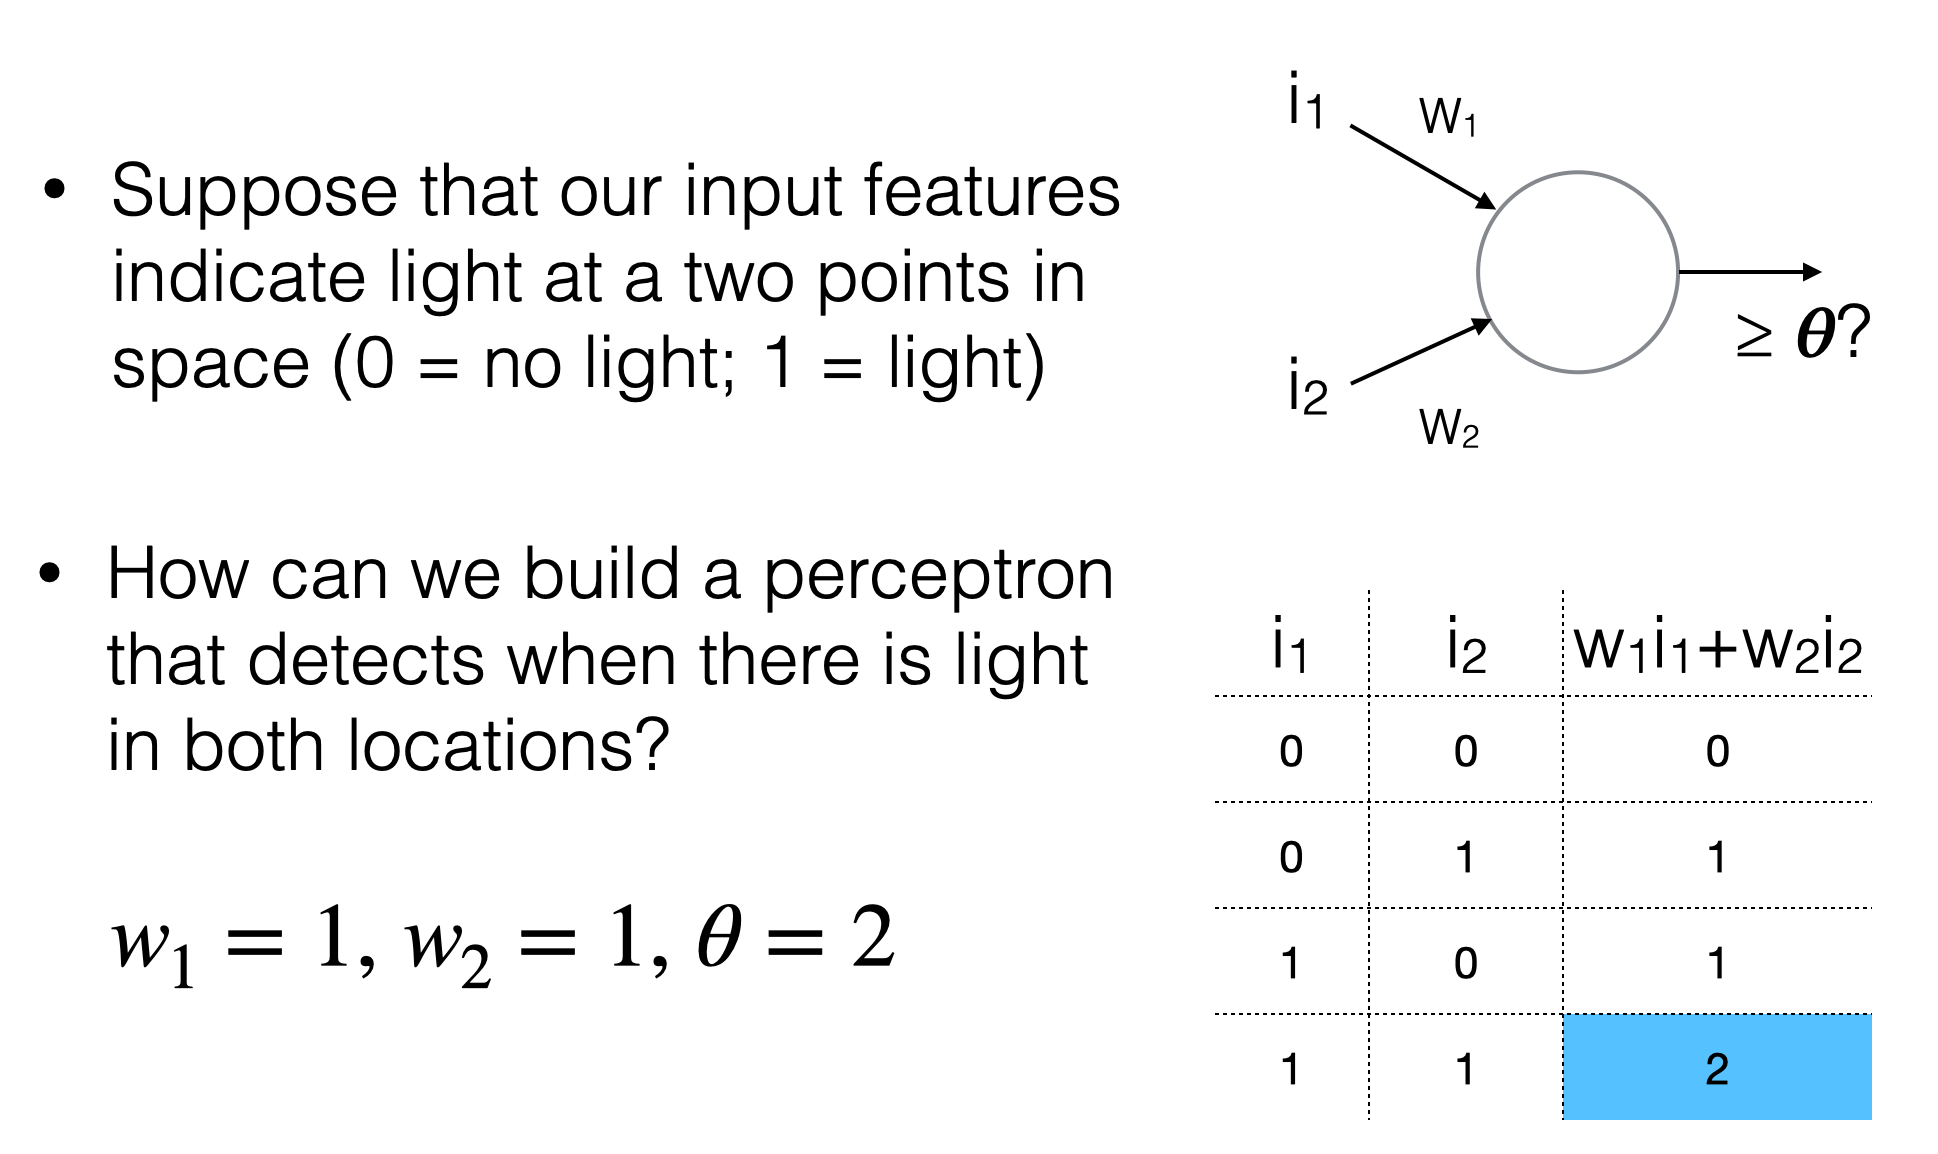
\includegraphics[height=0.8\textheight]{figures/perceptron_keynote}
\end{frame}

\begin{frame}{Limitations of a perceptrons as logical gates}
    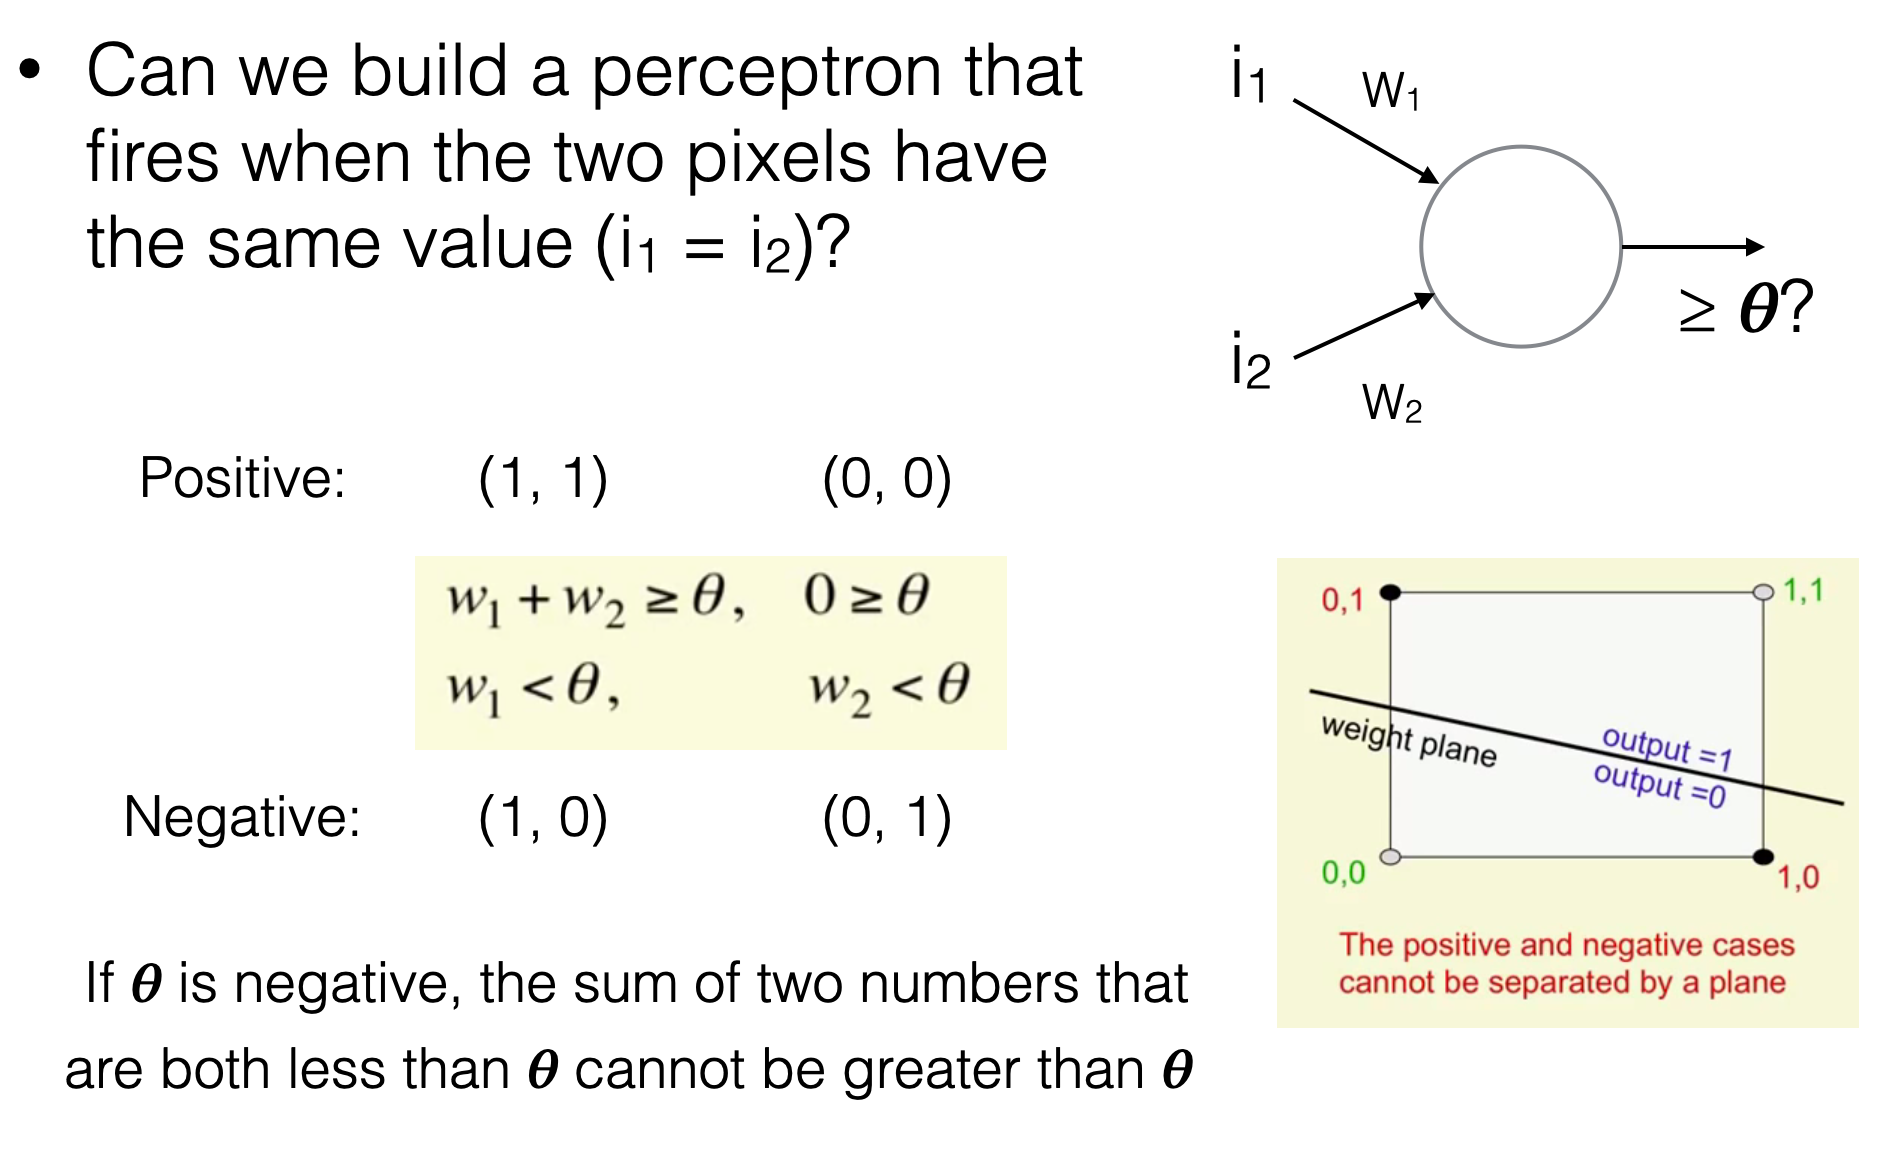
\includegraphics[height=0.8\textheight]{figures/perceptron_limitations_keynote}
\end{frame}

\begin{frame}{Multilayer perceptron}
    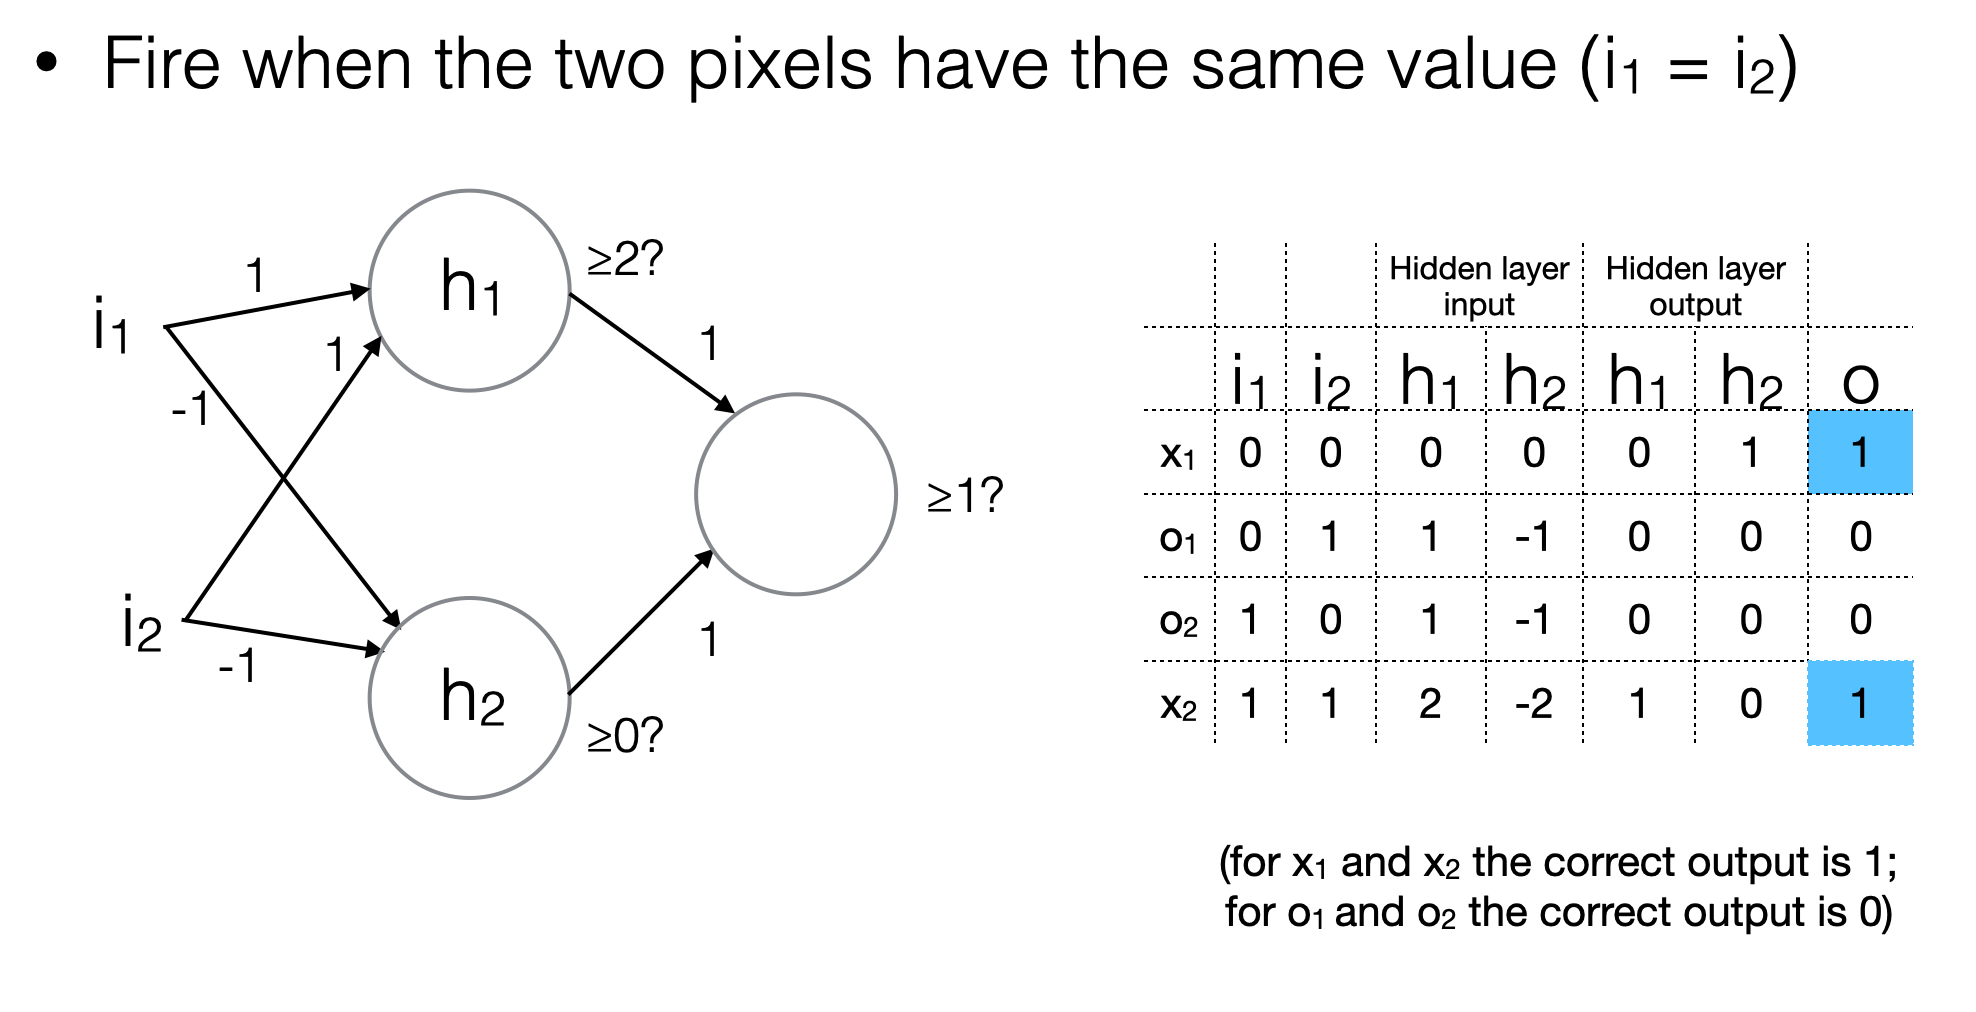
\includegraphics[height=0.8\textheight]{figures/perceptron_solution_keynote}
\end{frame}

\begin{frame}{Multilayer perceptron}
    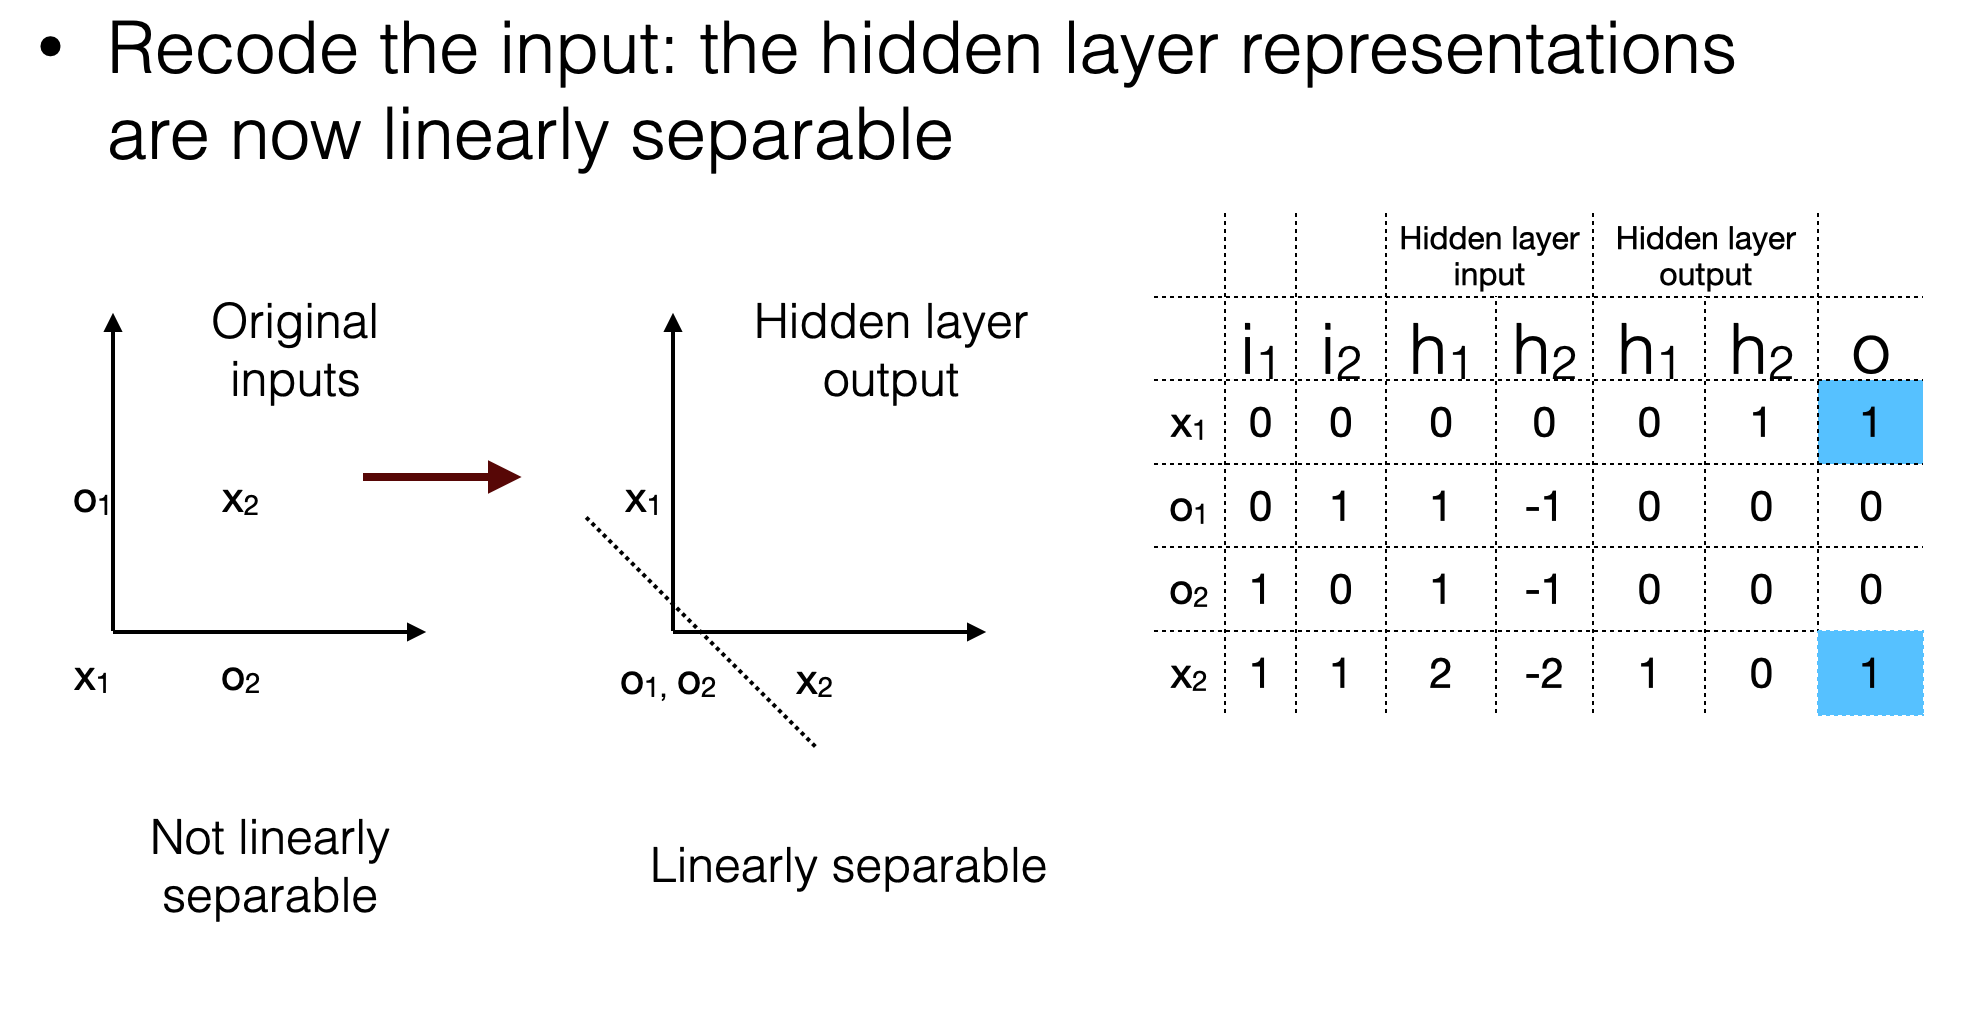
\includegraphics[height=0.8\textheight]{figures/perceptron_recoding}
\end{frame}

\begin{frame}
{Decomposing the problem into predefined subproblems}
\begin{center}
\def\layersep{2.5cm}
\begin{tikzpicture}[shorten >=1pt,->,draw=black!50, node distance=\layersep]
    \tikzstyle{every pin edge}=[<-,shorten <=1pt]
    \tikzstyle{neuron}=[circle,fill=black!25,minimum size=17pt,inner sep=0pt]
    \tikzstyle{input neuron}=[neuron, fill=green!50];
    \tikzstyle{output neuron}=[neuron, fill=red!50];
    \tikzstyle{hidden neuron}=[neuron, fill=blue!50];
    \tikzstyle{annot} = [text width=4em, text centered]

    % Draw the input layer nodes
    \foreach \name / \y / \text in {1/1/\#dishes, 2/2/price, 3/3/wine option, 4/4/zip code, 5/5/\#seats, 6/6/size}
    % This is the same as writing \foreach \name / \y in {1/1,2/2,3/3,4/4}
        \node[input neuron, pin=left:\text] (I-\name) at (0,-\y) {};

    % Draw the hidden layer nodes
    \foreach \name / \y in {1,...,3}
        \path[yshift=-1.3cm]
            node[hidden neuron] (H-\name) at (\layersep,-\y cm) {};

    % Draw the output layer node
    \node[output neuron,node distance=4cm,pin={[pin edge={->}]right:Popularity}, right of=H-2] (O) {};

    % Connect every node in the input layer with every node in the
    % hidden layer.
%    \foreach \source in {1,...,6}
%        \foreach \dest in {1,...,3}
%            \path (I-\source) edge (H-\dest);
	\foreach \source in {1,2,3}
		\path (I-\source) edge (H-1);
	\foreach \source in {4}
		\path (I-\source) edge (H-2);
	\foreach \source in {5,6}
		\path (I-\source) edge (H-3);

    % Connect every node in the hidden layer with the output layer
    \foreach \source in {1,...,3}
        \path (H-\source) edge (O);

    % Annotate the layers
    \node[annot,above of=H-1, node distance=2.5cm] (hl) {Intermediate features};
    \node[annot,left of=hl] {Input features};
    \node[annot,right of=hl, node distance=4cm] {Output};
    
    % Annotate the hidden nodes
    \foreach \h / \text in {1/food quality, 2/walkable, 3/noise}
    		\node[annot, above of=H-\h, node distance=0.5cm] {$h_\h$};
    \foreach \h / \text in {1/food quality, 2/walkable, 3/noise}
    		\node[annot, right of=H-\h, node distance=2cm, text width=4cm] {\text};
\end{tikzpicture}
\end{center}
\note[item]{Let's try to represent our model as a graph. So we have nodes representing each input, nodes representing the intermediate predictors which takes in a subset of inputs, and the node representing the linear classifier that computes the output.}
\note[item]{The subproblems are manually specified based on our knowledge of the problem. 
In fact, feature engineering is an important step when building practical ML models, but in this course so far we have ignored that part and assume they are given to use.
But we don't always have this knowledge, or our features aren't good, or we simply want to automate as many steps as possible.
It would be desirable if we can directly learn these subproblems.}
\end{frame}

\begin{frame}
{Learned intermediate features}
\begin{center}
\def\layersep{2.5cm}
\begin{tikzpicture}[shorten >=1pt,->,draw=black!50, node distance=\layersep]
    \tikzstyle{every pin edge}=[<-,shorten <=1pt]
    \tikzstyle{neuron}=[circle,fill=black!25,minimum size=17pt,inner sep=0pt]
    \tikzstyle{input neuron}=[neuron, fill=green!50];
    \tikzstyle{output neuron}=[neuron, fill=red!50];
    \tikzstyle{hidden neuron}=[neuron, fill=blue!50];
    \tikzstyle{annot} = [text width=4em, text centered]

    % Draw the input layer nodes
    \foreach \name / \y / \text in {1/1/\#dishes, 2/2/price, 3/3/wine option, 4/4/zip code, 5/5/\#seats, 6/6/size}
    % This is the same as writing \foreach \name / \y in {1/1,2/2,3/3,4/4}
        \node[input neuron, pin=left:\text] (I-\name) at (0,-\y) {};

    % Draw the hidden layer nodes
    \foreach \name / \y in {1,...,3}
        \path[yshift=-1.3cm]
            node[hidden neuron] (H-\name) at (\layersep,-\y cm) {};

    % Draw the output layer node
    \node[output neuron,node distance=4cm,pin={[pin edge={->}]right:Popularity}, right of=H-2] (O) {};

    % Connect every node in the input layer with every node in the
    % hidden layer.
    \foreach \source in {1,...,6}
        \foreach \dest in {1,...,3}
            \path (I-\source) edge (H-\dest);

    % Connect every node in the hidden layer with the output layer
    \foreach \source in {1,...,3}
        \path (H-\source) edge (O);

    % Annotate the layers
    \node[annot,above of=H-1, node distance=2.5cm] (hl) {\textcolor{blue}{Hidden} layer};
    \node[annot,left of=hl] {Input layer};
    \node[annot,right of=hl, node distance=4cm] {Output layer};
    
    % Annotate the hidden nodes
    \foreach \h / \text in {1/food quality, 2/walkable, 3/noise}
    		\node[annot, above of=H-\h, node distance=0.5cm] {$h_\h$};
\end{tikzpicture}
\end{center}
\note[item]{Let's re-draw our graph. Without knowing the structure of the subproblems, we'll have to give all inputs to the intermediate predictors, and hope it can learn some features automatically. But it will be hard to tell what they learned exactly, so we will call these nodes \emph{hidden units}, and they form the \emph{hidden layer}. Similarly, the input nodes form the input layer and the last layer is the output layer.}
\end{frame}

\begin{frame}
{Neural networks}
\textbf{Key idea}: learn the intermediate features.
\begin{description}[Feature engineering]
\item<+->[Feature engineering]
Manually specify $\phi(x)$ based on domain knowledge and learn the weights:
\begin{align}
f(x) = {\color{red}w}^T\phi(x) .
\end{align}

\item<+->[Feature learning]
Learn both the features ($K$ hidden units) and the weights:
\begin{align}
h(x) &= \pb{{\color{red}h_1}(x), \ldots, {\color{red}h_K}(x)} , \\
f(x) &= {\color{red}w}^T h(x)
\end{align}
\end{description}
\note[item]{Let's write our model down in equations now.}
\note[item]{Typically, we specify $\phi$ based on domain knowledge.}
\note[item]{NN learn both the features and the weights.}
\note[item]{But we haven't parametrized $h$ yet.}
\end{frame}

\begin{frame}{Feature learning example}
\begin{itemize}
    \item<1-> A filter convolves over the image and looks for the highest pattern match.
    \item<2-> Traditionally, people use Gabor filters or other image feature extractors, e.g. SIFT, SURF, etc, and an SVM on top for image classification.
    \item<3-> Neural networks take in images and can learn the filters that are the most useful for solving the tasks. Likely more efficient than hand engineered features.
\end{itemize}
\begin{center}
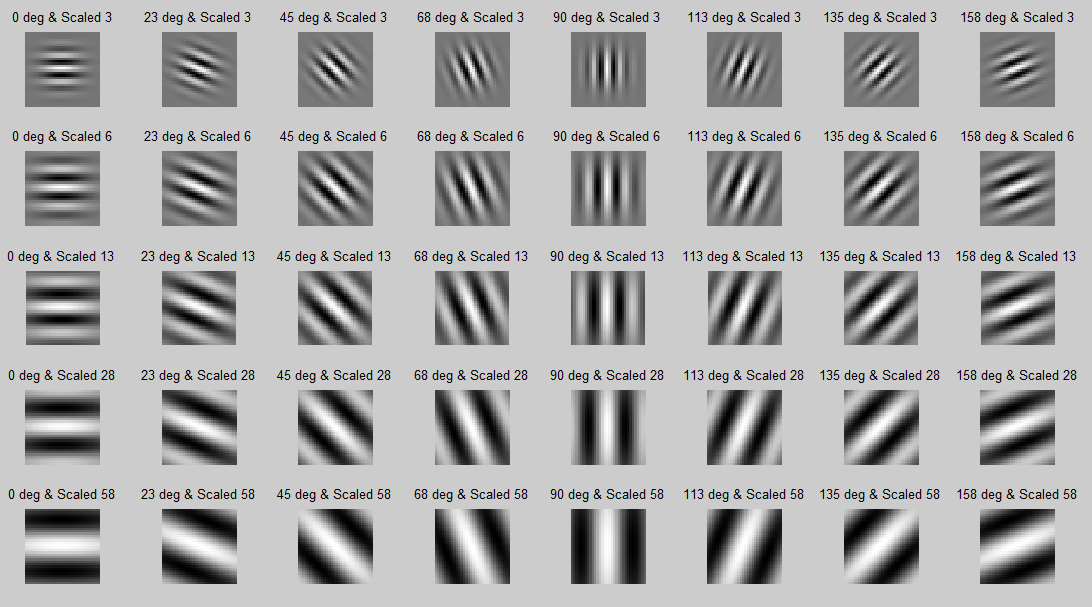
\includegraphics[height=3cm]{figures/gabor.png}
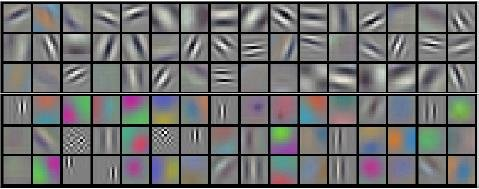
\includegraphics[height=3cm]{figures/alexnet.jpg}
\end{center}
\end{frame}

\begin{frame}{Inspiration: The brain}
\begin{itemize}
\item Our brain has about 100 billion ($10^{11}$) neurons, each of which communicates (is connected) to $\sim 10^4$ other neurons, with non-linear computations.
\end{itemize}
\vspace{0.2cm}
\begin{figure}
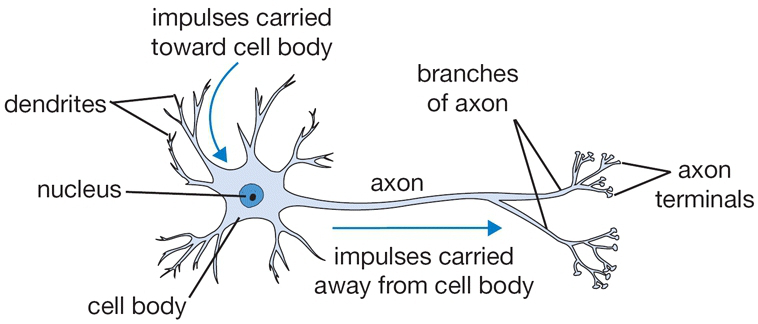
\includegraphics[width=0.76\linewidth]{figures/brain_neuron}
\caption{The basic computational unit of the brain:  Neuron}
\end{figure}
% \end{itemize}
\end{frame}

\begin{frame}{Inspiration: The brain}
  \begin{itemize}
    \item Neurons receive input signals and accumulate voltage. After some threshold they will fire spiking responses.
  \end{itemize}
  \begin{figure}
    \centering
    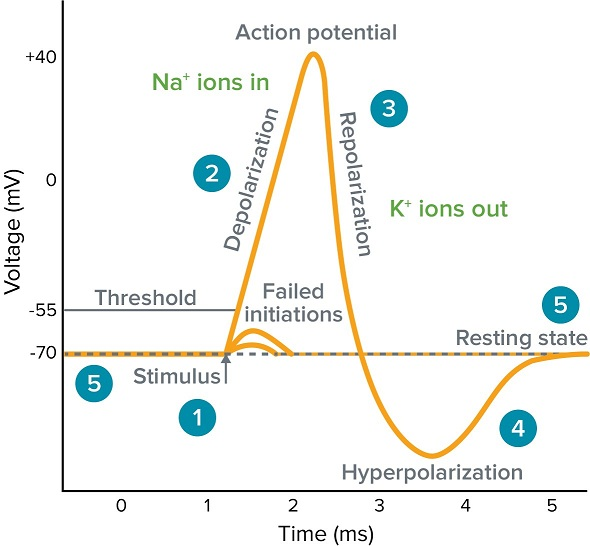
\includegraphics[width=0.4\textwidth]{figures/what-is-action-potential.jpg}
  \end{figure}
\end{frame}

\begin{frame}
{Activation function}
\begin{itemize}[<+->]
% \item How should we parametrize the $h_i$'s? Can they be linear?
\item We can model a simpler computation by using ``activation function''.
\item It applies a non-linearity on the inputs and ``fires'' after some threshold.
\onslide<+->{
\begin{align}
h_i(x) = {\color{blue}\sigma}(v_i^T x) .
\end{align}
}
% \item<.-> $\sigma$ is a \emph{nonlinear} \textbf{activation function}
\item Some possible activation functions:
\begin{itemize}
    \item $\text{sign}$ function (as in classic perceptron)? \alarm{Non-differentiable}.
\item \emph{Differentiable} approximations: sigmoid functions.
\begin{itemize}[<.->]
\item E.g., logistic function, hyperbolic tangent function.
\end{itemize}
\end{itemize}
\item Two-layer neural network (one \textcolor{blue}{hidden layer} and one  \textcolor{Green}{output layer}) with $K$ hidden units:
\begin{align}
f(x) &= \sum_{k=1}^{K} {\color{Green}w_k} h_k(x) = \sum_{k=1}^K {\color{Green}w_k} \sigma({\color{blue}v_k}^T x)
\end{align}
\end{itemize}
\note[item]{Recall that $h$ is an intermediate predictor. How about the sign function such that $h$ would output the result of a binary classifier.}
\note[item]{Sigmoid function is S-shaped functions that approximate sign function. (draw)}
\note[item]{Let's write down our two-layer network. In the output layer, we have a linear combination of the hidden units. Each hidden units compute a linear combination of its inputs followed by an activation function.}
\note[item]{Without the activation function this is just a linear model. What do we gain from these nonlinear activation functions? Let's look at how well a two layer NN approximate different functions.}
\end{frame}

\begin{frame}{Activation Functions}

\begin{itemize}
\item The \textbf{hyperbolic tangent} is a common activation function:
\[
\sigma(x)=\tanh\left(x\right).
\]
\end{itemize}
\begin{figure}
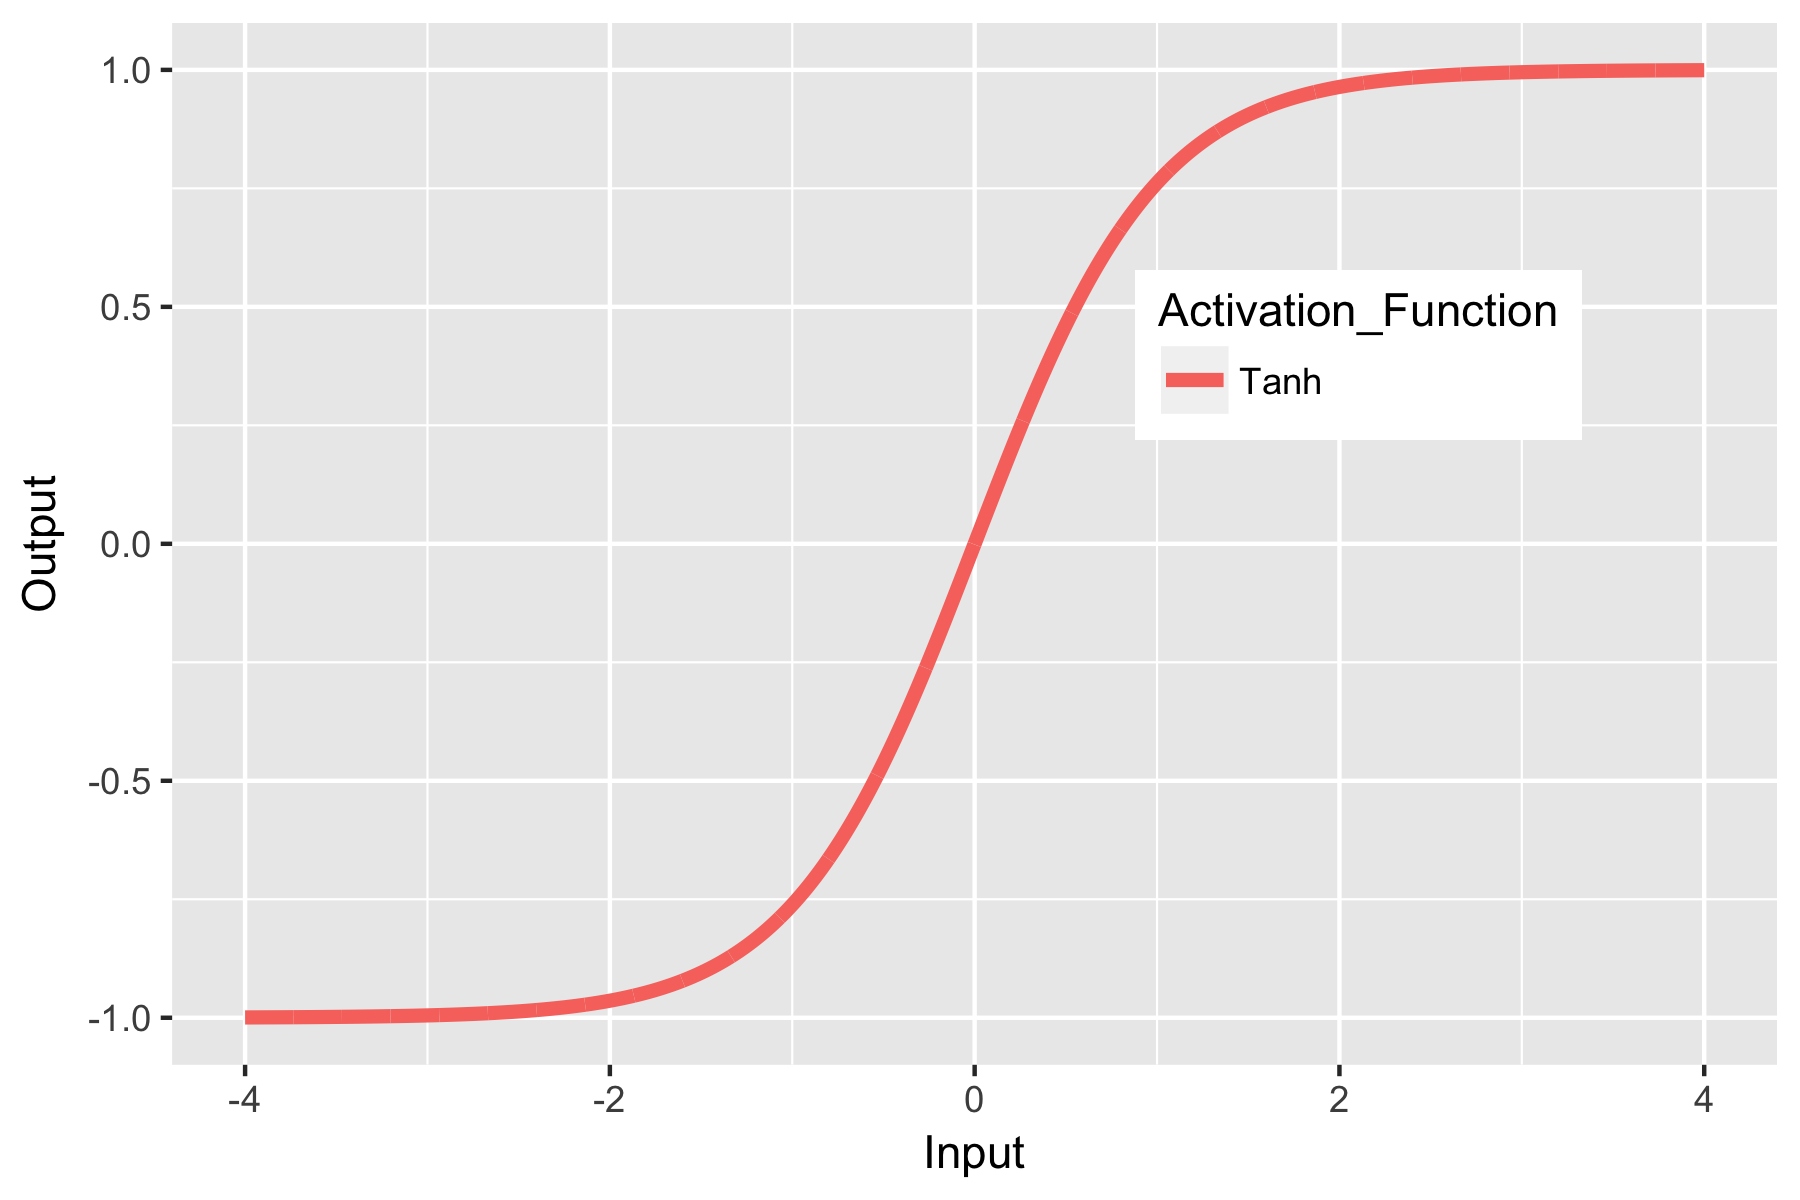
\includegraphics[height=0.55\textheight]{figures/activationFn-Tanh}
\end{figure}
\end{frame}
%
\begin{frame}{Activation Functions}
\begin{itemize}
\item More recently, the \textbf{rectified linear} (\textbf{ReLU}) function has been very
popular:
\[
\sigma(x)=\max(0,x).
\]
\item Faster to calculate this function and its derivatives
\item Often more effective in practice
\end{itemize}
\begin{figure}
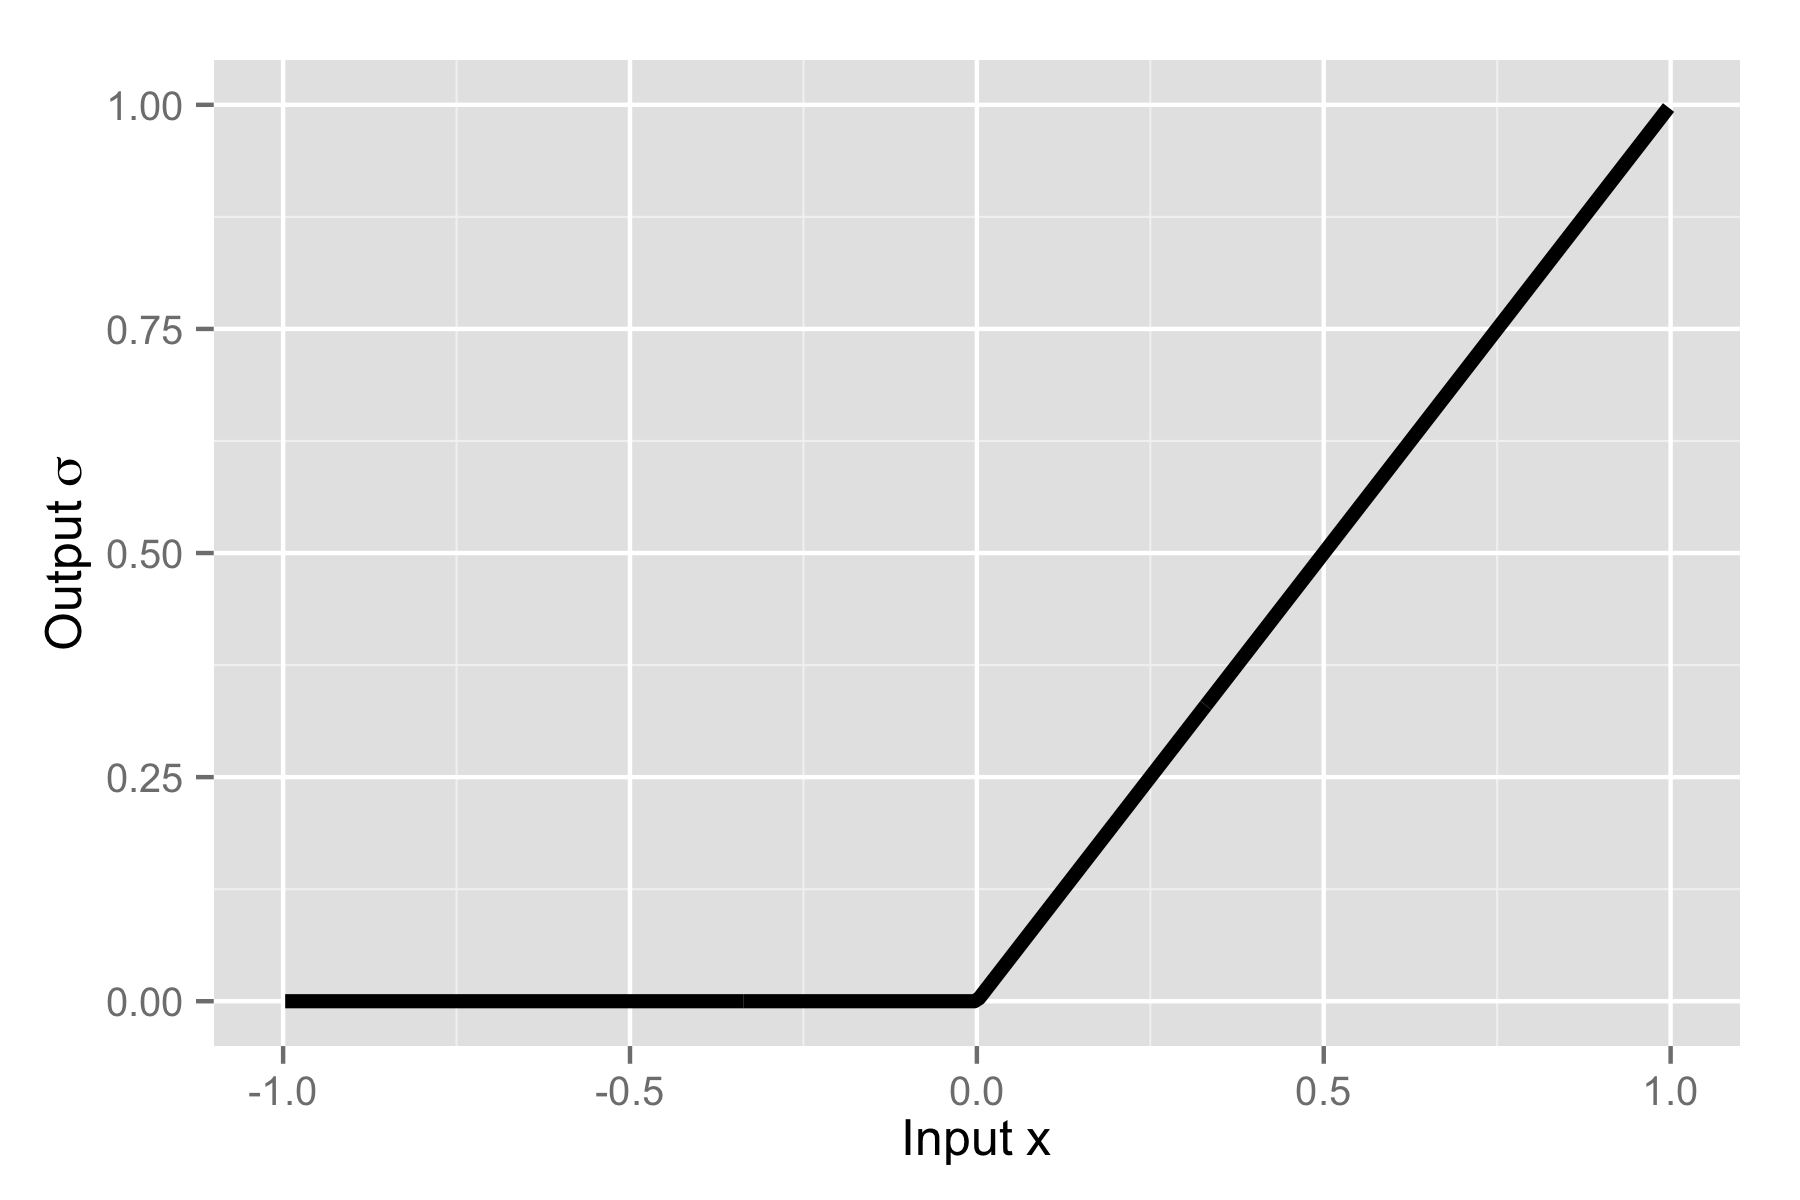
\includegraphics[height=0.55\textheight]{figures/activationFn-Rectified_Linear} 
\end{figure}
\end{frame}

\subsection{Approximation Properties of Two-layer Neural Networks}
\begin{frame}{Approximation Ability: $f(x)=x^{2}$}
\begin{itemize}
\item 3 hidden units; tanh activation functions 
\item Blue dots are training points; dashed lines are hidden unit outputs;
final output in red.
\end{itemize}
\centering
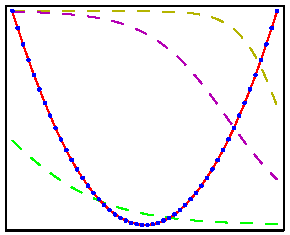
\includegraphics[height=0.6\textheight]{{figures/Figure5_3a.pdf}} 

\let\thefootnote\relax\footnotetext{\tiny{From Bishop's \emph{Pattern Recognition and Machine Learning}, Fig 5.3 }}
\note[item]{Convex.}
\end{frame}
%
\begin{frame}{Approximation Ability: $f(x)=\sin(x)$}
\begin{itemize}
\item 3 hidden units; logistic activation function
\item Blue dots are training points; dashed lines are hidden unit outputs;
final output in red.
\end{itemize}
\centering
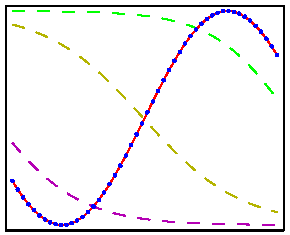
\includegraphics[height=0.6\textheight]{{figures/Figure5_3b}.pdf} 

\let\thefootnote\relax\footnotetext{\tiny{From Bishop's \emph{Pattern Recognition and Machine Learning}, Fig 5.3 }}
\note[item]{Nonconvex but smooth.}
\end{frame}
%
\begin{frame}{Approximation Ability: $f(x)=\left|x\right|$}
\begin{itemize}
\item 3 hidden units; logistic activation functions 
\item Blue dots are training points; dashed lines are hidden unit outputs;
final output in red.
\end{itemize}
\centering
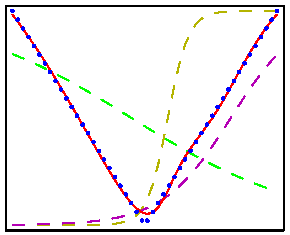
\includegraphics[height=0.6\textheight]{{figures/Figure5_3c}.pdf} 

\let\thefootnote\relax\footnotetext{\tiny{From Bishop's \emph{Pattern Recognition and Machine Learning}, Fig 5.3 }}
\note[item]{Non-smooth.}
\end{frame}
%
%\begin{frame}{Approximation Ability: $f(x)=\ind{x>0}$}
%\begin{itemize}
%\item 3 hidden units; logistic activation function
%\item Blue dots are training points; Dashed lines are hidden unit outputs;
%Final output in Red.
%\end{itemize}
%\centering
%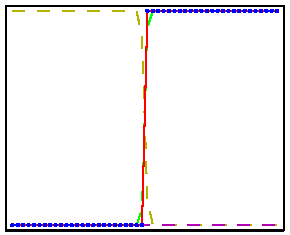
\includegraphics[height=0.6\textheight]{{figures/Figure5_3d}.pdf} 
%
%%%\let\thefootnote\relax\footnotetext{\tiny{From Bishop's \emph{Pattern Recognition and Machine Learning}, Fig 5.3 }}
%\note[item]{Not continuous}
%\end{frame}

\begin{frame}
{Universal approximation theorem}
\begin{theorem}[Universal approximation theorem]
A neural network with one \alarm{possibly huge hidden layer} $\hat{F}(x)$ can 
approximate \emph{any continuous function} $F(x)$ on a closed and bounded subset of $\reals^d$ under mild assumptions on the activation function, \ie $\forall \epsilon>0$, there exists an integer $N$ s.t.
\begin{align}
\hat{F}(x) = \sum_{i=1}^{\color{red}N} w_i \sigma(v_i^Tx + b_i)
\end{align}
satisfies $\vert \hat{F}(x) - F(x)\vert < \epsilon$.
\end{theorem}
\end{frame}

\begin{frame}{Universal approximation theorem}
    \begin{itemize}[<+->]
\item For the theorem to work, the number of hidden units needs to be exponential in $d$
\item The theorem doesn't tell us how to find the parameters of this network
\item It doesn't explain why practical neural networks work, or tell us how to build them
\end{itemize}
\end{frame}

\subsection{Deep neural networks}
\begin{frame}
    {Deep neural networks}
\begin{itemize}
    \item Wider: more hidden units (as in the approximation theorem).
\item Deeper: more hidden layers.
\end{itemize}
\begin{center}
\def\layersep{2.5cm}
\begin{tikzpicture}[shorten >=1pt,->,draw=black!50, node distance=\layersep]
    \tikzstyle{every pin edge}=[<-,shorten <=1pt]
    \tikzstyle{neuron}=[circle,fill=black!25,minimum size=17pt,inner sep=0pt]
    \tikzstyle{input neuron}=[neuron, fill=green!50];
    \tikzstyle{output neuron}=[neuron, fill=red!50];
    \tikzstyle{hidden neuron}=[neuron, fill=blue!50];
    \tikzstyle{annot} = [text width=4em, text centered]

    % Draw the input layer nodes
    \foreach \name / \y / \text in {1/1/1, 2/2/2, 3/3/, 4/4/d-1, 5/5/d}{
    		\ifthenelse{\y=3}
    		{\node[input neuron, pin=left:$\vdots$] (I-\name) at (0,-\y) {}}
        {\node[input neuron, pin=left:$x_{\text}$] (I-\name) at (0,-\y) {}}
	;}
    % Draw the hidden layer nodes
    \foreach \name / \y in {1,...,4}
        \path[yshift=-.5cm]
            node[hidden neuron] (H-\name) at (\layersep,-\y cm) {};
            
    % Draw the hidden layer nodes
    \foreach \name / \y in {1,...,3}
        \path[yshift=-1cm]
            node[hidden neuron] (H2-\name) at (2*\layersep,-\y cm) {};

    % Draw the output layer node
    \node[output neuron,pin={[pin edge={->}]right:score}, right of=H2-2] (O) {};

    % Connect every node in the input layer with every node in the
    % hidden layer.
    \foreach \source in {1,...,5}
        \foreach \dest in {1,...,4}
            \path (I-\source) edge (H-\dest);
    \foreach \source in {1,...,4}
        \foreach \dest in {1,...,3}
            \path (H-\source) edge (H2-\dest);

    % Connect every node in the hidden layer with the output layer
    \foreach \source in {1,...,3}
        \path (H2-\source) edge (O);

    % Annotate the layers
    \node[annot,above of=H-1, node distance=1.3cm] (hl) {{Hidden} layers};
    \node[annot,left of=hl] {Input layer};
    \node[annot,right of=hl, node distance=5cm] {Output layer};
    
\end{tikzpicture}
\end{center}
\note[item]{It's pretty easy to extend the two layer NN we just talked about. We can either add more hidden layers, or more hidden units in each layer. Modern neural networks usually have many hidden layers. If the nodes in any two adjacent layers are fully connected, we call it a MLP or FFNN.}
\end{frame}

\begin{frame}{Multilayer Perceptron (MLP): formal definition}
\begin{itemize}
\item \textbf{Input space}: $\cx=\reals^{d}$$\qquad$\textbf{Output space}
$\cy=\reals^{k}$ (for $k$-class classification).

\item Let $\sigma:\reals\to\reals$ be an activation function
(e.g. $\tanh$ or ReLU).

\item Let's consider an MLP of $L$ hidden layers, each having $m$ hidden units.

\pause

\item First hidden layer is given by
\[
h^{(1)}(x)=\sigma\left(W^{(1)}x+b^{(1)}\right),
\]
for parameters $W^{(1)}\in\reals^{m\times d}$ and $b\in\reals^{m}$,
and where $\sigma\left(\cdot\right)$ is applied to each entry of
its argument.
\end{itemize}
\note[item]{Let's write down a MLP with $L$ hidden layer in math.}
\note[item]{The first layer is just the activation function composed with an affine transformation of the input.}
\note[item]{Note that $\sigma$ operates on each element of the vector.}
\end{frame}
%
\begin{frame}{Multilayer Perceptron (MLP): formal definition}
\begin{itemize}[<+->]
\item Each subsequent hidden layer takes the \emph{output $o\in\reals^{m}$ of
previous layer} and produces
\[
h^{(j)}({\color{blue}o^{(j-1)}})=\sigma\left(W^{(j)}{\color{blue}o^{(j-1)}}+b^{(j)}\right),\text{ for }j=2,\ldots,L
\]
where $W^{(j)}\in\reals^{m\times m}$, $b^{(j)}\in\reals^{m}$.

\item Last layer is an \emph{affine} mapping (no activation function): 
\[
a(o^{(L)})=W^{(L+1)}o^{(L)}+b^{(L+1)},
\]
where $W^{(L+1)}\in\reals^{k\times m}$ and $b^{(L+1)}\in\reals^{k}$.

\item The full neural network function is given by the \emph{composition} of
layers:
\begin{align}
f(x) &= \left(a\circ h^{(L)}\circ\cdots\circ h^{(1)}\right)(x)
\end{align}

\item Typically, the last layer gives us a score. How do we perform classification?
\end{itemize}
\end{frame}
%

\begin{frame}{What did we do in multinomial logistic regression?}
\begin{itemize}
\item From each $x$, we compute a linear score function for each class:
\[
x\mapsto\left(\left\langle w_{1},x\right\rangle ,\ldots,\left\langle w_{k},\right\rangle \right)\in\reals^{k}
\]
\item We need to map this $\reals^{k}$ vector into a probability vector
$\theta$.

\pause{}
\item The \textbf{softmax function} maps scores $s=\left(s_{1},\ldots,s_{k}\right)\in\reals^{k}$
to a categorical distribution\textbf{: 
\[
\left(s_{1},\ldots,s_{k}\right)\mapsto\theta=\softmax\left(s_{1},\ldots,s_{k}\right)=\left(\frac{\exp\left(s_{1}\right)}{\sum_{i=1}^{k}\exp\left(s_{i}\right)},\ldots,\frac{\exp\left(s_{k}\right)}{\sum_{i=1}^{k}\exp\left(s_{i}\right)}\right)
\]
}
\end{itemize}
\end{frame}

\begin{frame}{Nonlinear Generalization of Multinomial Logistic Regression}
\begin{itemize}
\item From each $x$, we compute a non-linear score function for each class:
\[
x\mapsto\left(f_1(x) ,\ldots, f_k(x) \right)\in\reals^{k}
\]
where $f_i$'s are the outputs of the last hidden layer of a neural network.
\item {Learning}: Maximize the log-likelihood of training data
\[
\argmax_{f_{1},\ldots,f_{k}}\sum_{i=1}^{n}\log\left[\softmax\left(f_{1}(x),\ldots,f_{k}(x)\right)_{y_{i}}\right].
\]

%\item Unfortunately, this objective function is not concave or convex. 
%
%\item But we can still use gradient methods to find a good local optimum.
\end{itemize}
\end{frame}

\begin{frame}
{Interim discussion}
\begin{itemize}
\item With the right representations, we can turn nonlinear problems into linear ones
\item The goal of represenation learning is to automatically discover useful features from raw data
\pause
\item Building blocks:
\begin{description}[Hidden layer(s)]
\item[Input layer] no learnable parameters
\item[Hidden layer(s)] affine + \emph{nonlinear} activation function
\item[Output layer] affine (+ softmax)
\end{description}
\pause
\item A single, potentially huge hidden layer is sufficient to approximate any function
\item In practice, it is often helpful to have multiple hidden layers
\end{itemize}
\end{frame}


\section{Back-propagation}

\begin{frame}{Fitting the parameters of an MLP}
\begin{itemize}
\item \textbf{Input space}: $\cx=\reals$ 
\item \textbf{Output space}: $\cy=\reals$
\item \textbf{Hypothesis space}: MLPs with a single 3-node hidden layer:
\[
f(x)=w_{0}+w_{1}h_{1}(x)+w_{2}h_{2}(x)+w_{3}h_{3}(x),
\]
where 
\[
h_{i}(x)=\sigma(v_{i}x+b_{i})\text{ for }i=1,2,3,
\]
for some fixed activation function $\sigma:\reals\to\reals$. 


\item What are the parameters we need to fit?
\[
\pause b_{1},b_{2},b_{3},v_{1},v_{2},v_{3},w_{0},w_{1},w_{2},w_{3}\in\reals
\]
\end{itemize}
\note[item]{How do we learn these parameters?}
\end{frame}
%
%
\begin{frame}{Finding the best hypothesis}
\begin{itemize}[<+->]
\item As usual, we choose our prediction function using empirical risk minimization.
\item Our hypothesis space is parameterized by
\[
\theta=\left(b_{1},b_{2},b_{3},v_{1},v_{2},v_{3},w_{0},w_{1},w_{2},w_{3}\right)\in\Theta=\reals^{10}
\]
\item For a training set $(x_{1},y_{1}),\ldots,(x_{n},y_{n})$, our goal is to find
\[
\hat{\theta}=\argmin_{\theta\in\reals^{10}}\frac{1}{n}\sum_{i=1}^{n}\left(f(x_{i}; \theta)-y_{i}\right)^{2}.
\]
\end{itemize}
\end{frame}

\begin{frame}{How do we learn these parameters?}
    \begin{itemize}
\item For a training set $(x_{1},y_{1}),\ldots,(x_{n},y_{n})$, our goal is to find
\[
\hat{\theta}=\argmin_{\theta\in\reals^{10}}\frac{1}{n}\sum_{i=1}^{n}\left(f(x_{i}; \theta)-y_{i}\right)^{2}.
\]
\item We can use gradient descent
\item Is $f$ differentiable w.r.t. $\theta$? $f(x) = {\color{blue}w_{0}}+\sum_{i=1}^{3}{\color{blue}w_{i}}\tanh({\color{blue}v_{i}}x+{\color{blue}b_{i}})$.
    \pause
\item Is the loss convex in $\theta$? 
    \pause
    \begin{itemize}
    \item $\tanh$ is not convex
    \item Regardless of nonlinearity, the composition of convex functions is not necessarily convex
\end{itemize}

\item We might converge to a local minimum.
\end{itemize}
\end{frame}

\begin{frame}
{Gradient descent for (large) neural networks}
\begin{itemize}[<+->]
\item Mathematically, it's just \emph{partial derivatives}, which you can compute by hand using the \emph{chain rule}
\begin{itemize}[<.->]
\item In practice, this could be \alarm{time-consuming} and \alarm{error-prone}
\end{itemize}
\item Back-propagation computes gradients for neural networks (and other models) in a systematic and efficient way
\item We can visualize the process using \emph{computation graphs}, which
expose the structure of the computation (\textcolor{Green}{modularity} and \textcolor{Green}{dependency})
\end{itemize}
\end{frame}

\subsection{Partial Derivatives and the Chain Rule}

\begin{frame}
{Functions as nodes in a graph}
\begin{itemize}
\item We represent each component of the network as a \emph{node} that takes in a set of \emph{inputs} and produces a set of \emph{outputs}.
\item Example: $g:\reals^{p}\to\reals^{n}$.
\end{itemize}

\begin{columns}[t]
\column{.4\textwidth}
\begin{itemize}
\item Typical computation graph:
\end{itemize}
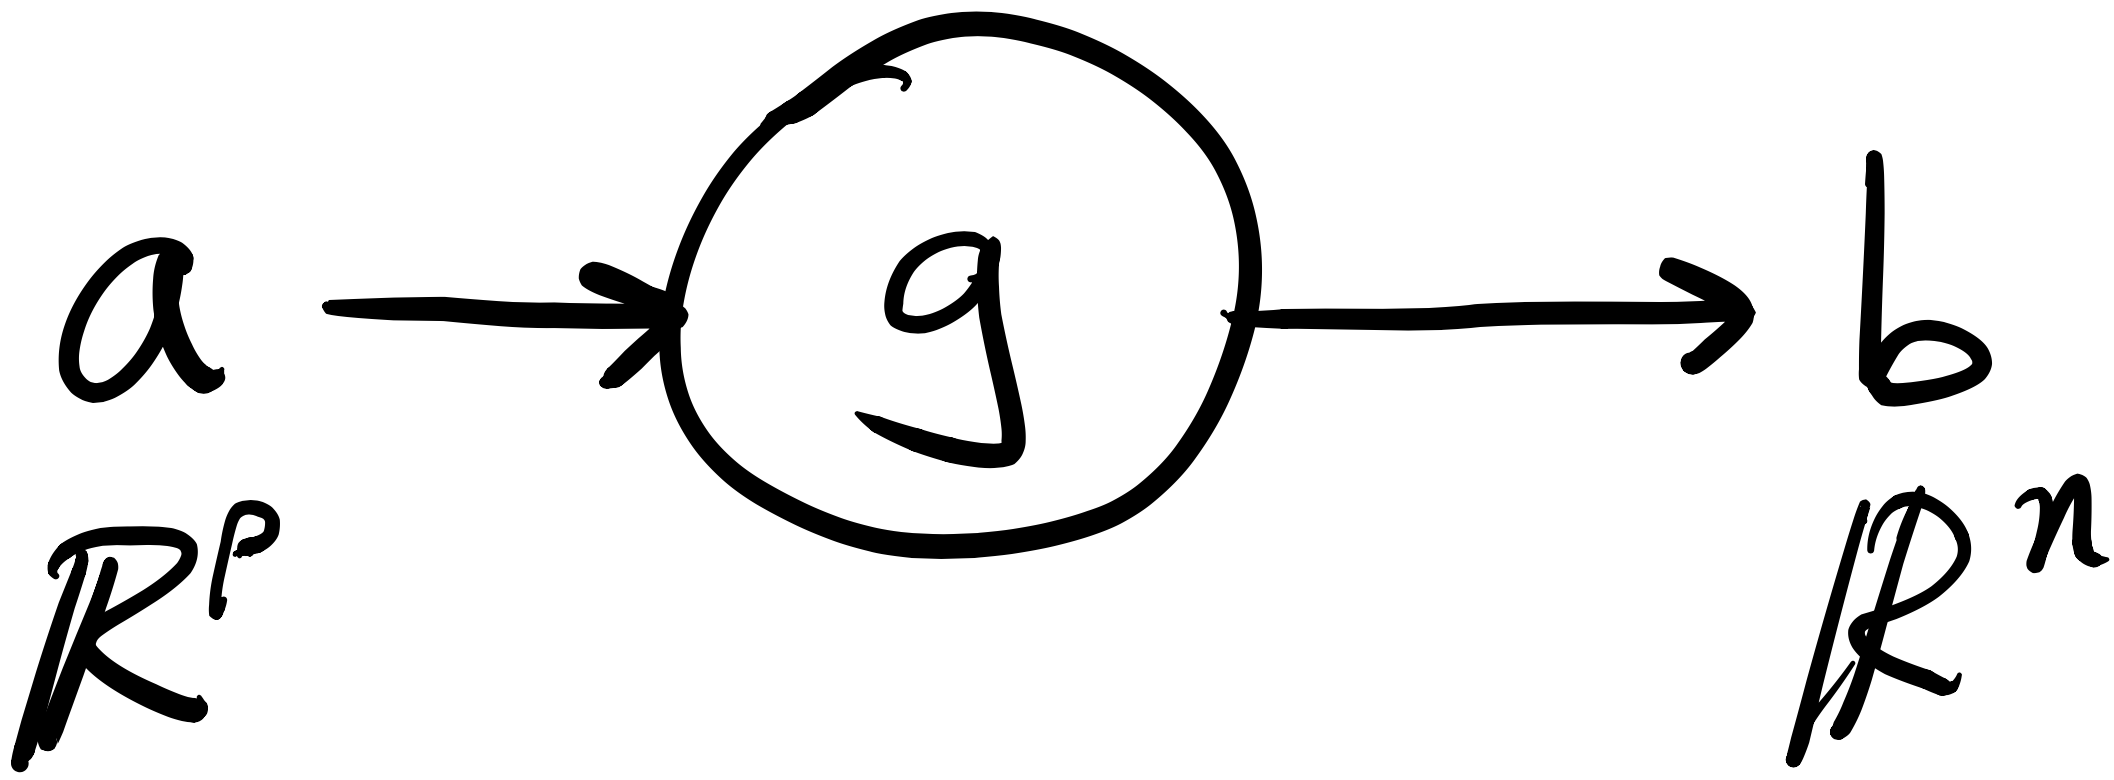
\includegraphics[scale=0.07]{figures/one-fn-comp-graph}

\pause{}

\column{.4\textwidth}
\begin{itemize}
\item Broken down by component:
\end{itemize}
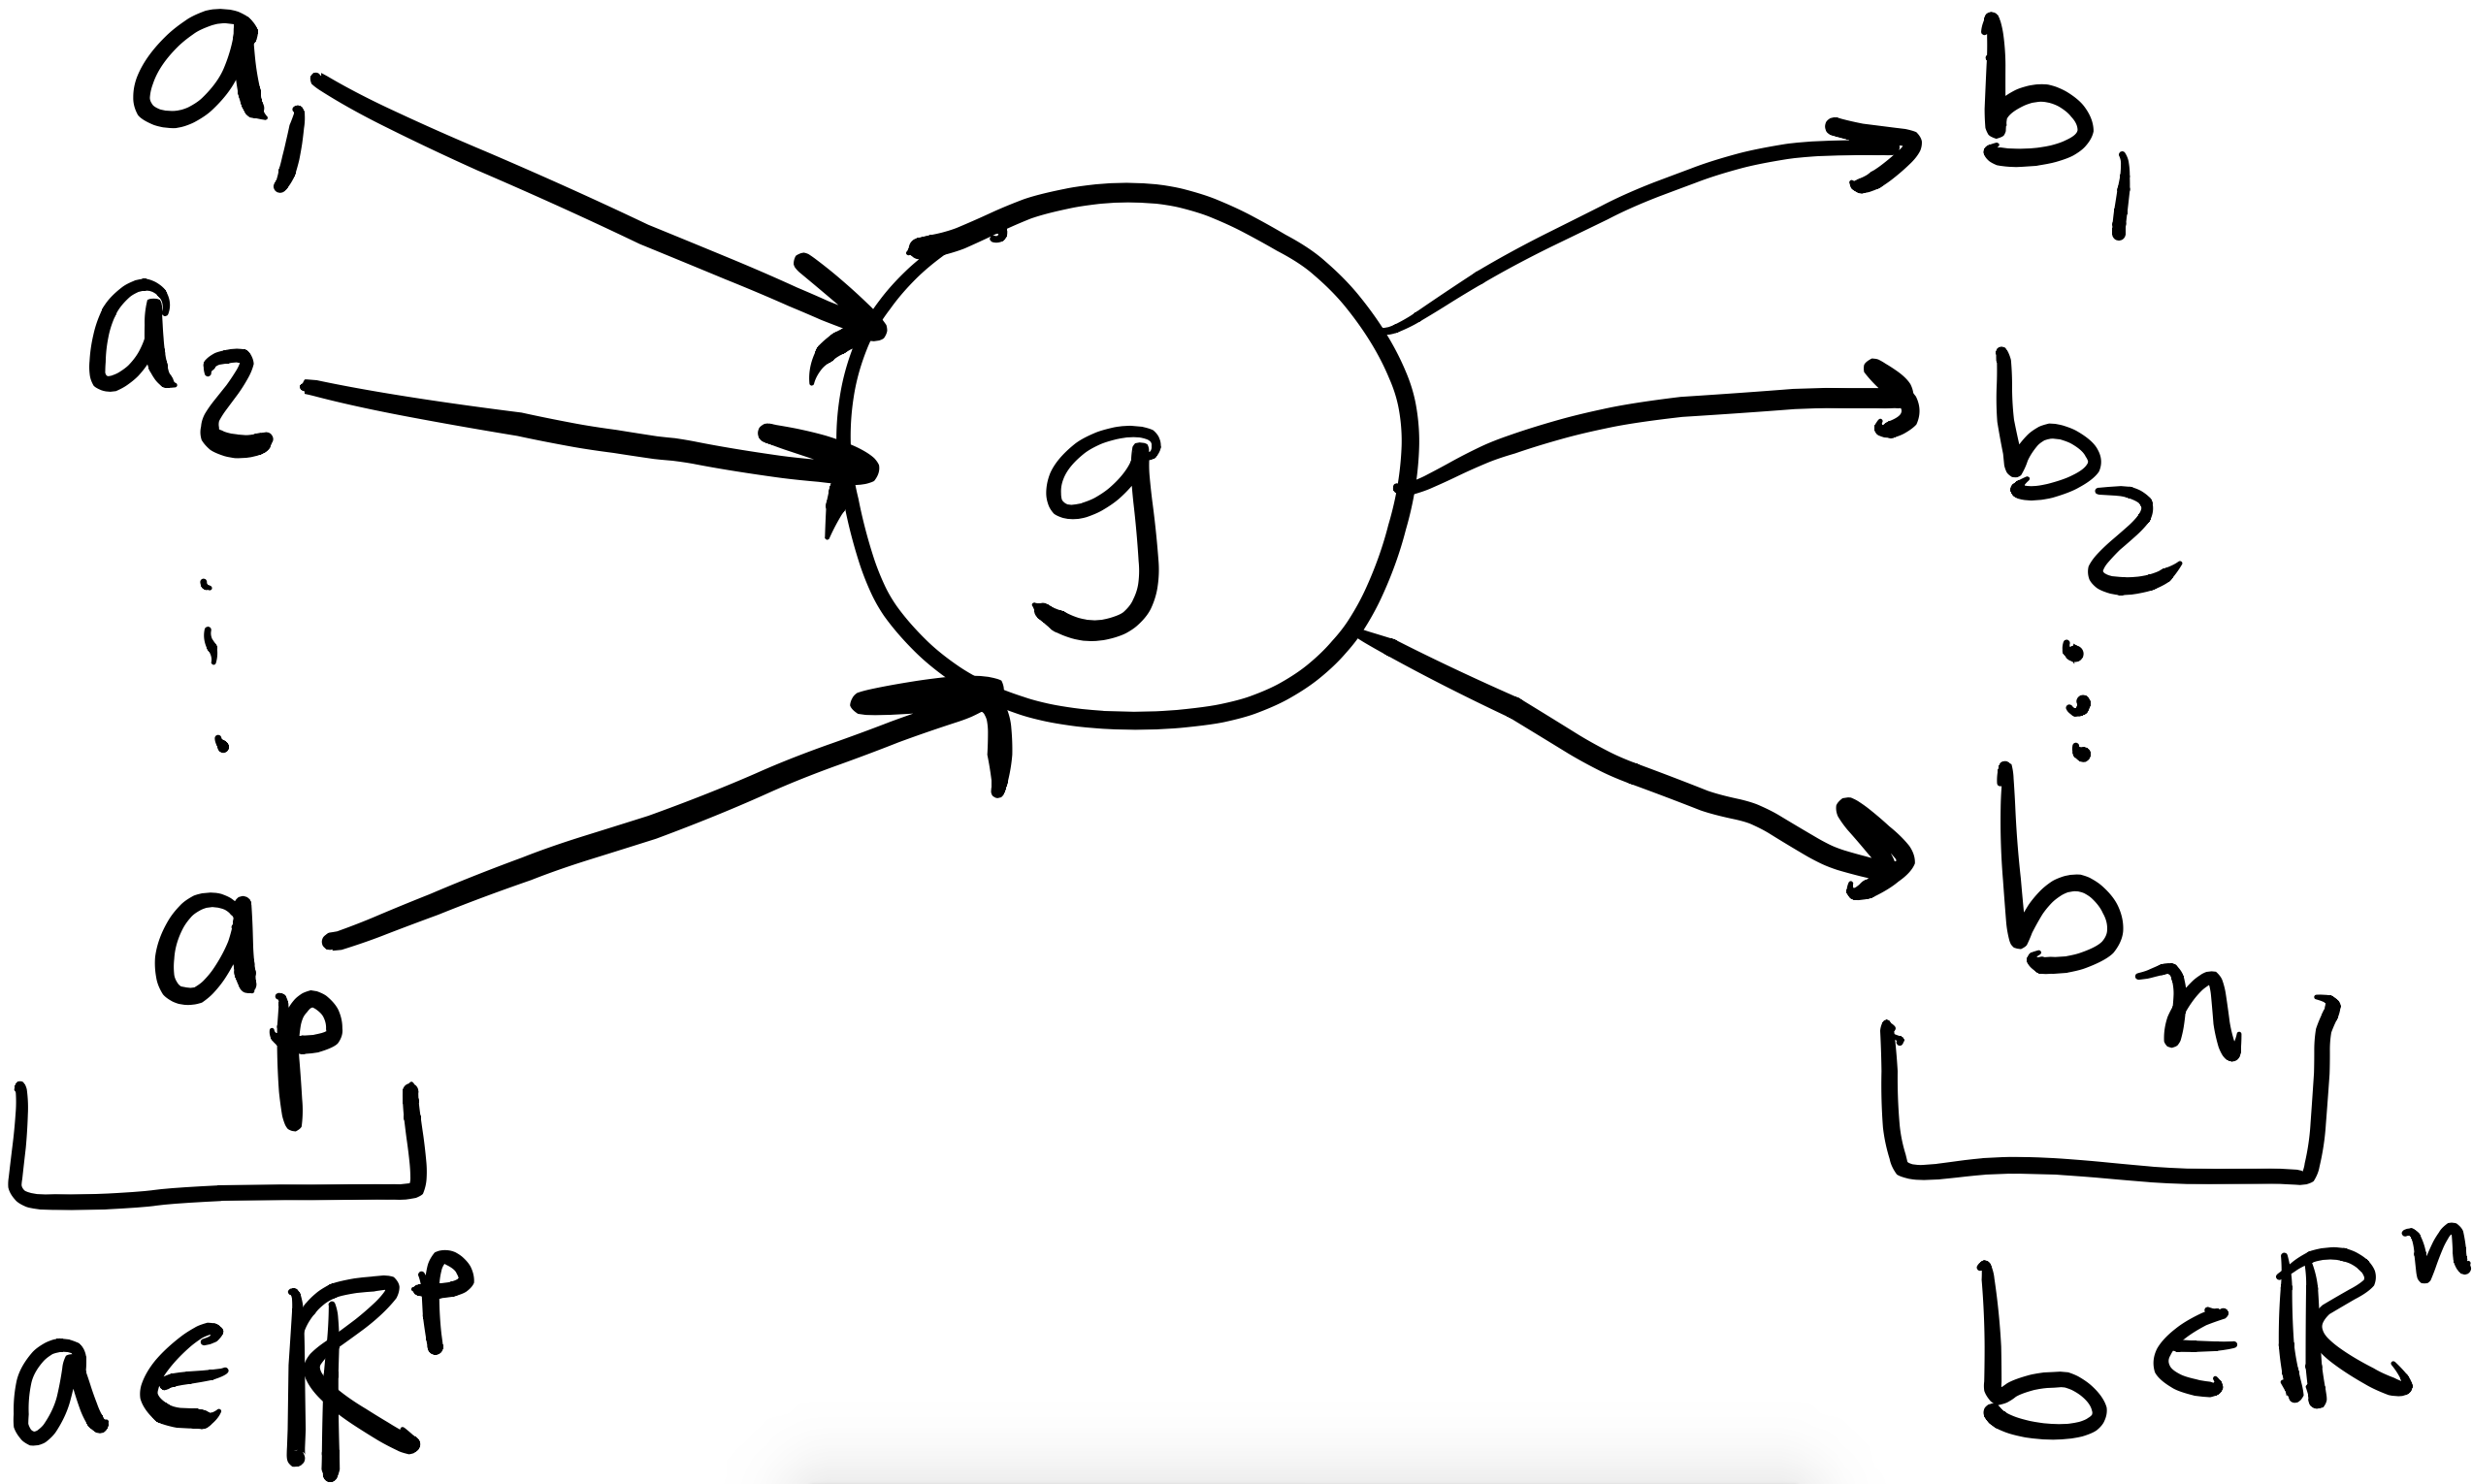
\includegraphics[scale=0.07]{figures/one-fn-comp-graph-partials}
\end{columns}
\note[item]{Conceptually, let's now think of functions as a graph. We have a node representing the computation happens in the function. The arrows or directed edges represent the input and output.}
\end{frame}

\begin{frame}{Partial derivatives of an affine function}
\begin{itemize}
\item Define the affine function $g(x)=Mx+c$, for $M\in\reals^{n\times p}$
and $c\in\reals$.
\end{itemize}
\begin{columns}[t]

\column{.35\textwidth}
\begin{figure}
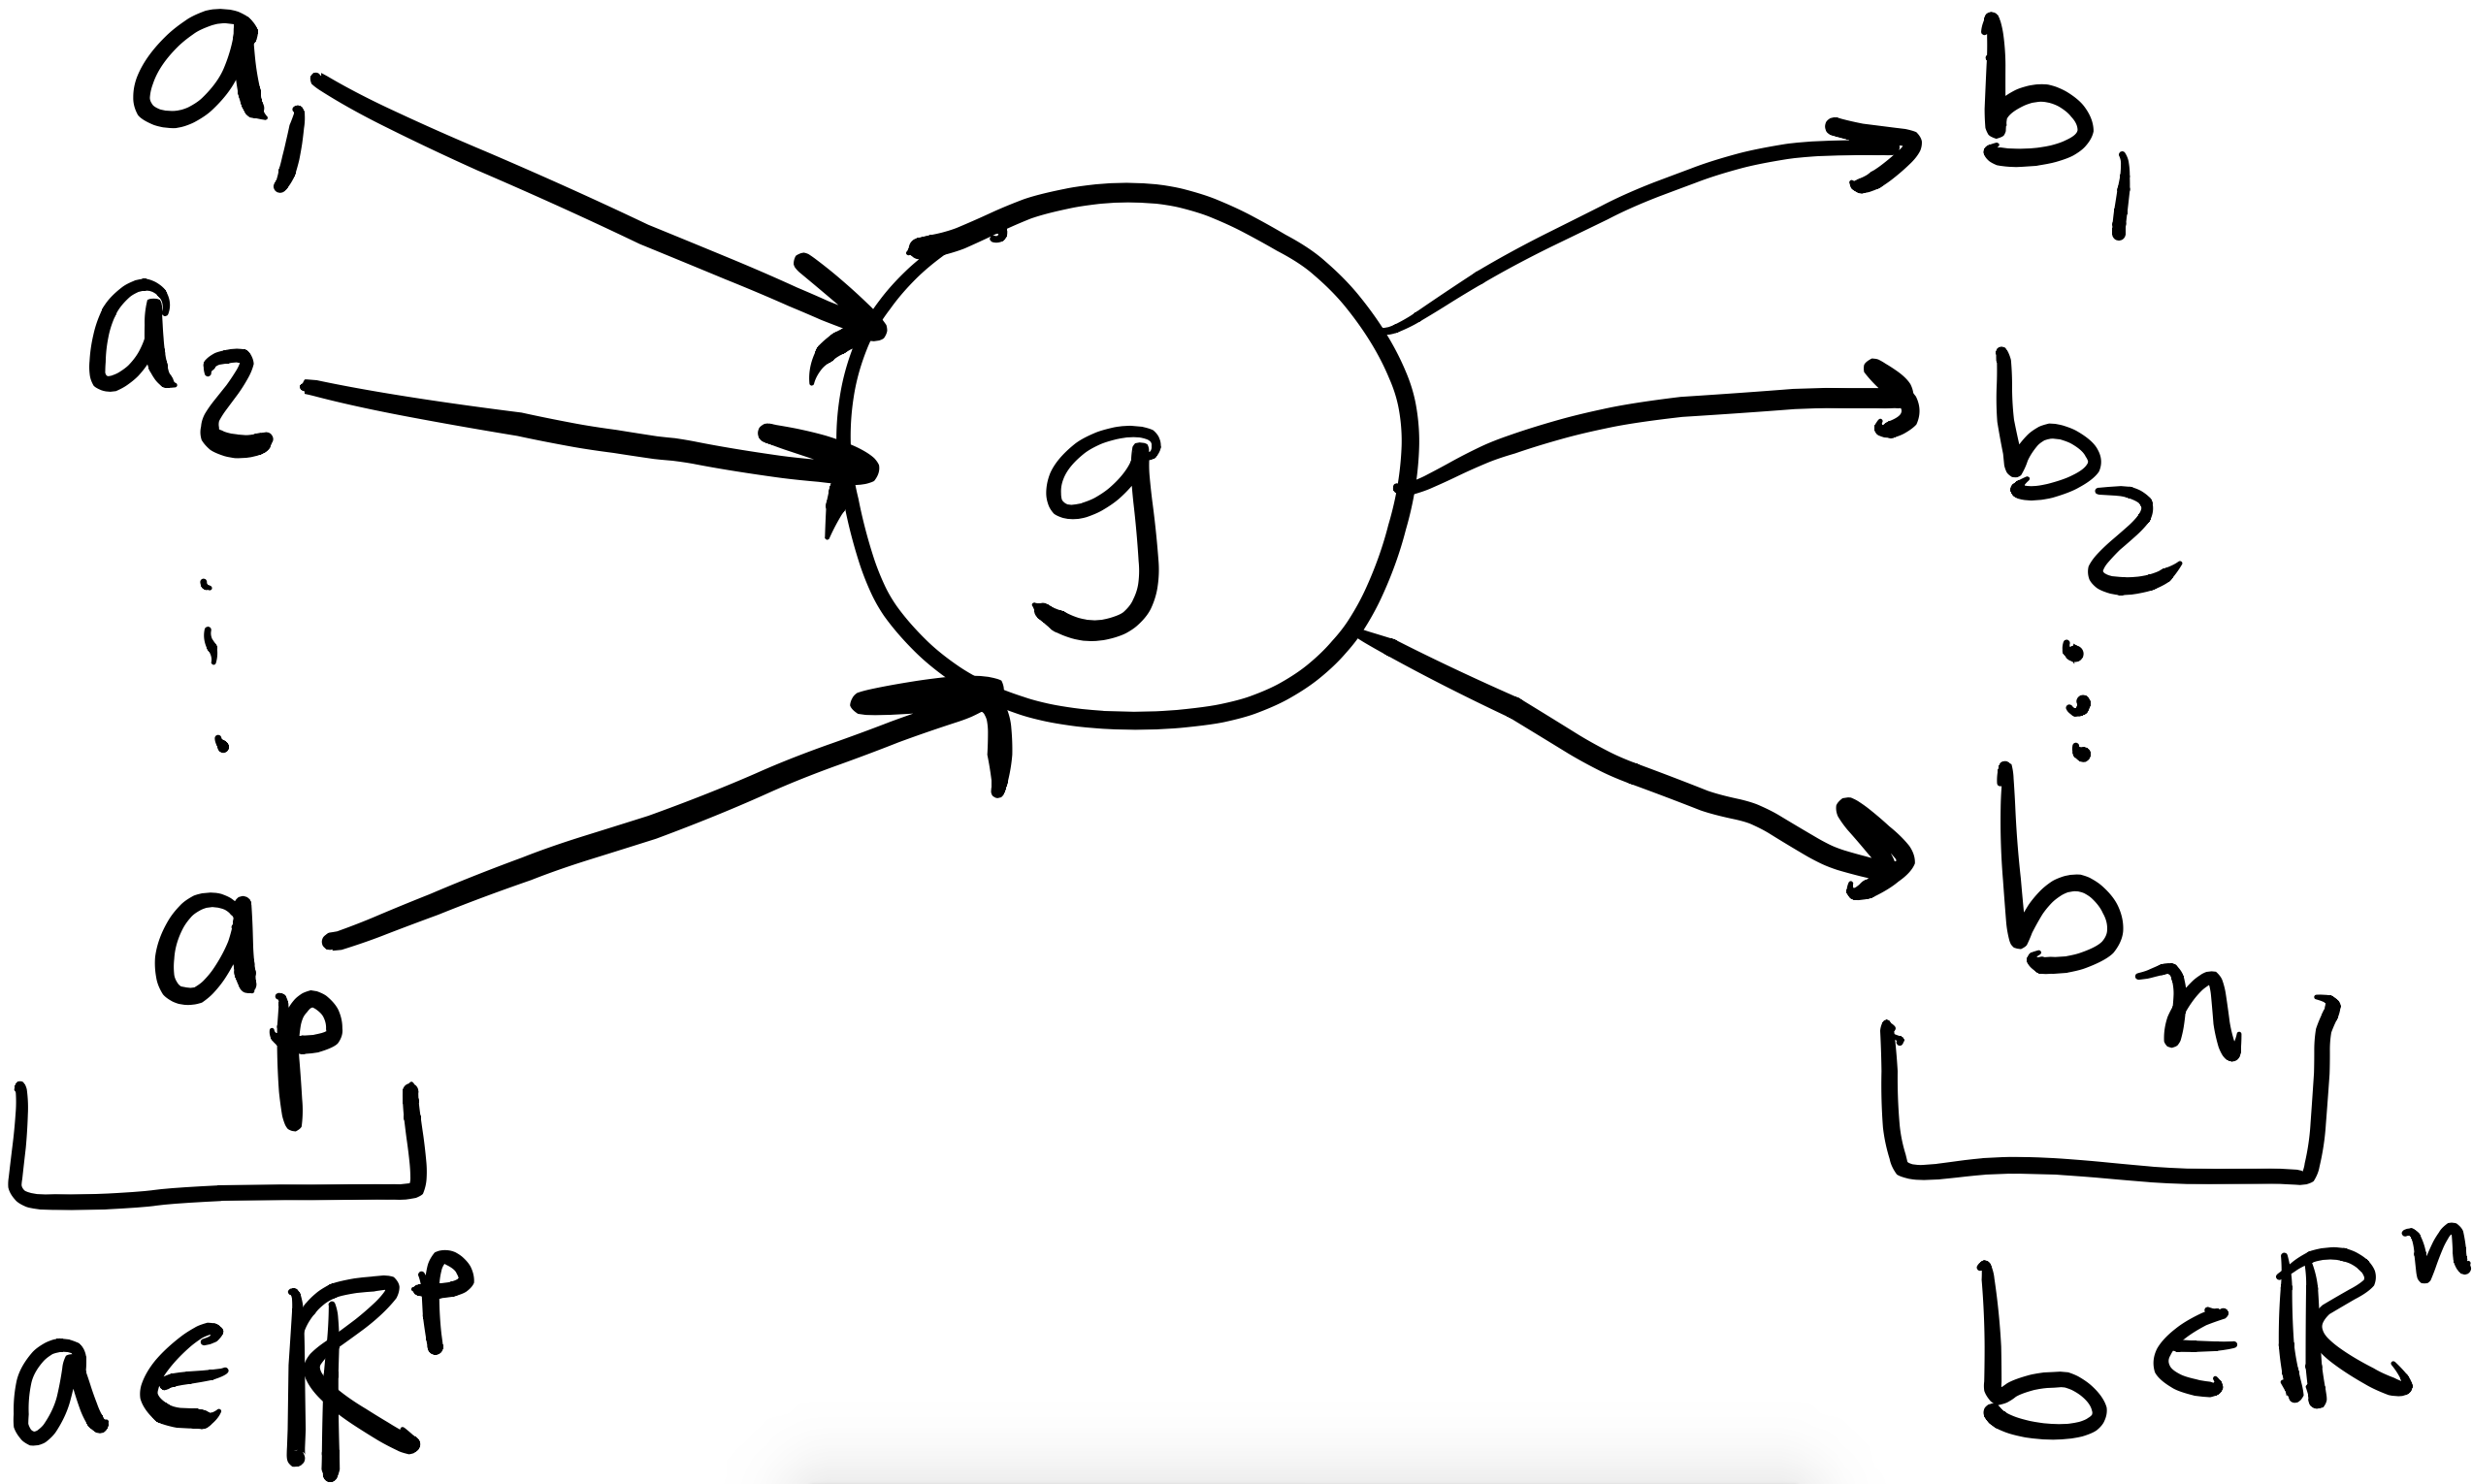
\includegraphics[scale=0.0625]{figures/one-fn-comp-graph-partials}
\end{figure}

\onslide<+->{
\column{.5\textwidth}
\begin{itemize}[<+->]
\item Let $b=g(a)=Ma+c$. What is $b_{i}$?
\item $b_{i}$ depends on the $i$th row of $M$: 
\[
b_{i}=\sum_{k=1}^{p}M_{ik}a_{k}+c_{i} .
\]
\item If $a_j \leftarrow a_j + {\color{blue}\delta}$, what is $b_i$?
\[
b_i \leftarrow b_i + {\color{blue}M_{ij}\delta} .
\]
\end{itemize}
}
\end{columns}
\onslide<+->{
    \vspace{-0.5cm}
The partial derivative/gradient measures \emph{sensitivity}:
If we perturb an input a little bit, how much does the output change?
}
\note[item]{Now, what is the meaning of partial derivatives on this graph. Let's consider the affine function as an example.}
\note[item]{Write the function.}
\note[item]{Draw matrix multiplication.}
\note[item]{$M_{ij} = \frac{\partial b_i}{\partial a_j}$}
\end{frame}

\begin{frame}{Partial derivatives in general}
\begin{itemize}
\item Consider a function $g:\reals^{p}\to\reals^{n}$.
\end{itemize}
\begin{columns}[t]

\column{.35\textwidth}
\begin{figure}
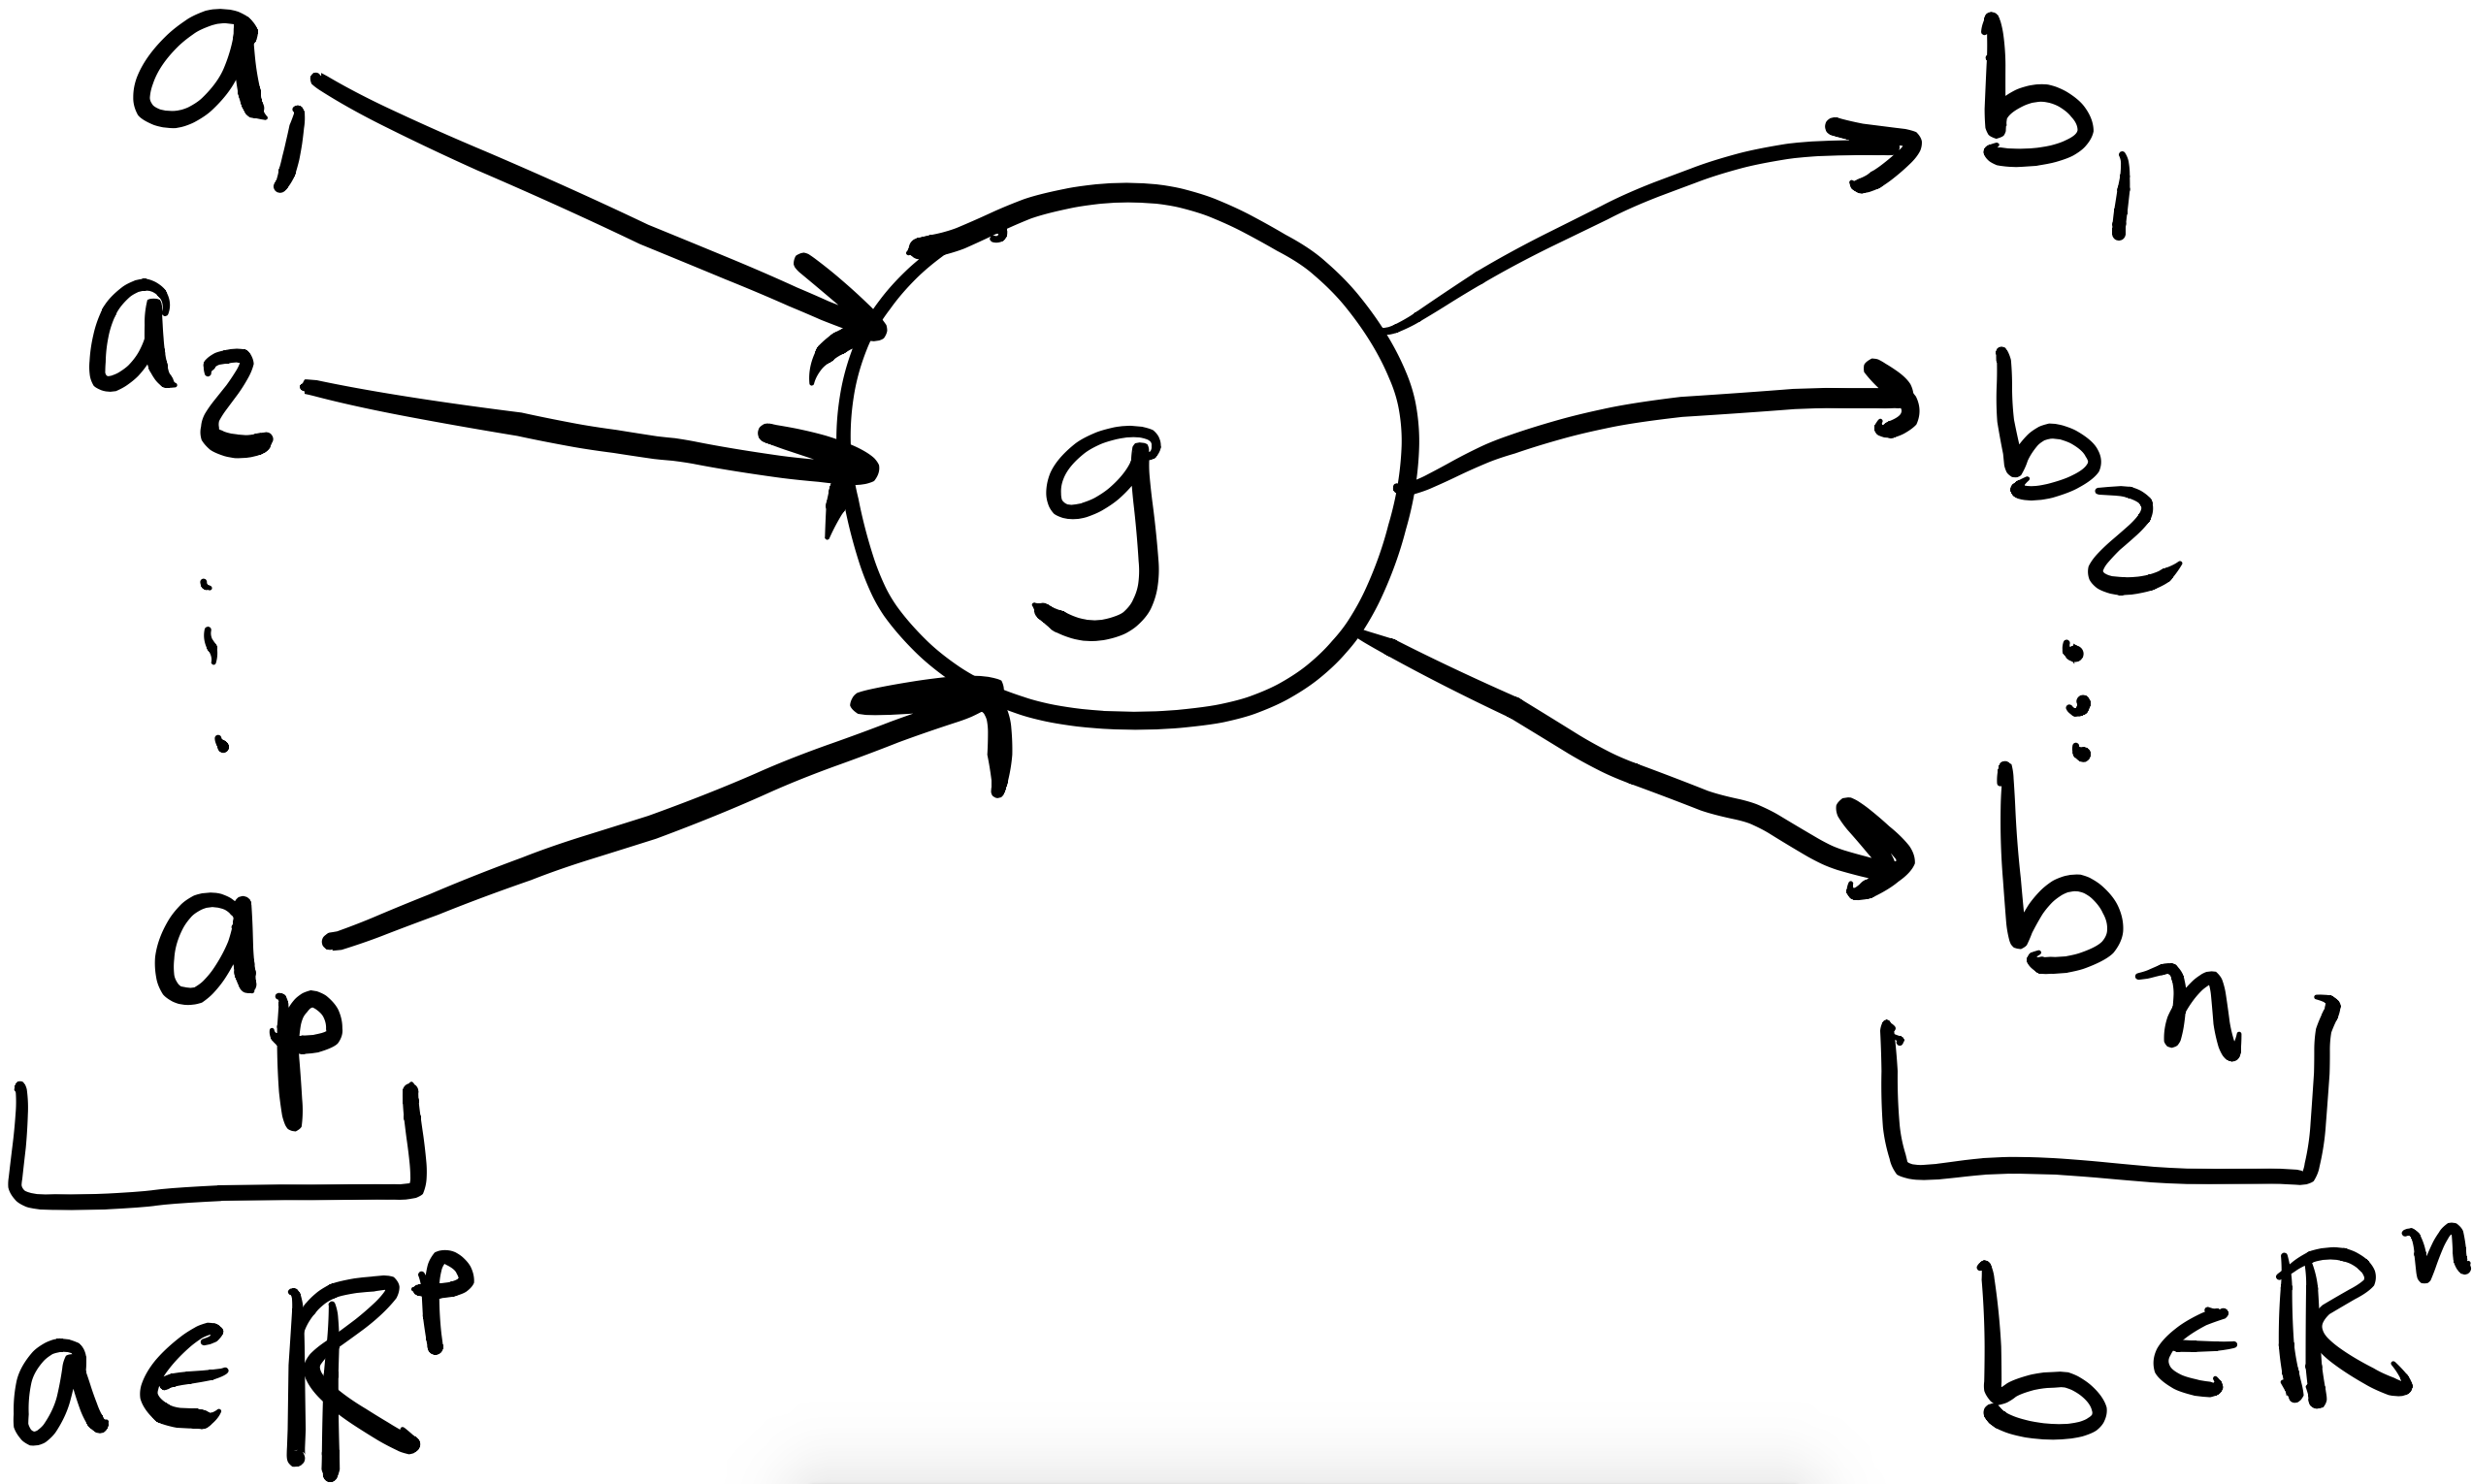
\includegraphics[scale=0.07]{figures/one-fn-comp-graph-partials}
\end{figure}

\column{.5\textwidth}
\begin{itemize}
\item Partial derivative $\frac{\partial b_{i}}{\partial a_{j}}$ is the
rate of change of $b_{i}$ as we change $a_{j}$
\item If we change $a_{j}$ slightly to
\[
a_{j}+{\color{blue}\delta} ,
\]
\item Then (for small $\delta$), $b_{i}$ changes to approximately
\[
b_{i}+{\color{blue}\frac{\partial b_{i}}{\partial a_{j}}\delta} .
\]
\end{itemize}
\end{columns}

\end{frame}

\begin{frame}
{Composing multiple functions}
\begin{itemize}
\item We have $g:\reals^{p}\to\reals^{n}$ and $f:\reals^{n}\to\reals^{m}$
\item $b=g(a)$, $c=f(b)$.
\end{itemize}
\begin{columns}
\begin{column}{0.5\textwidth}
\begin{figure}
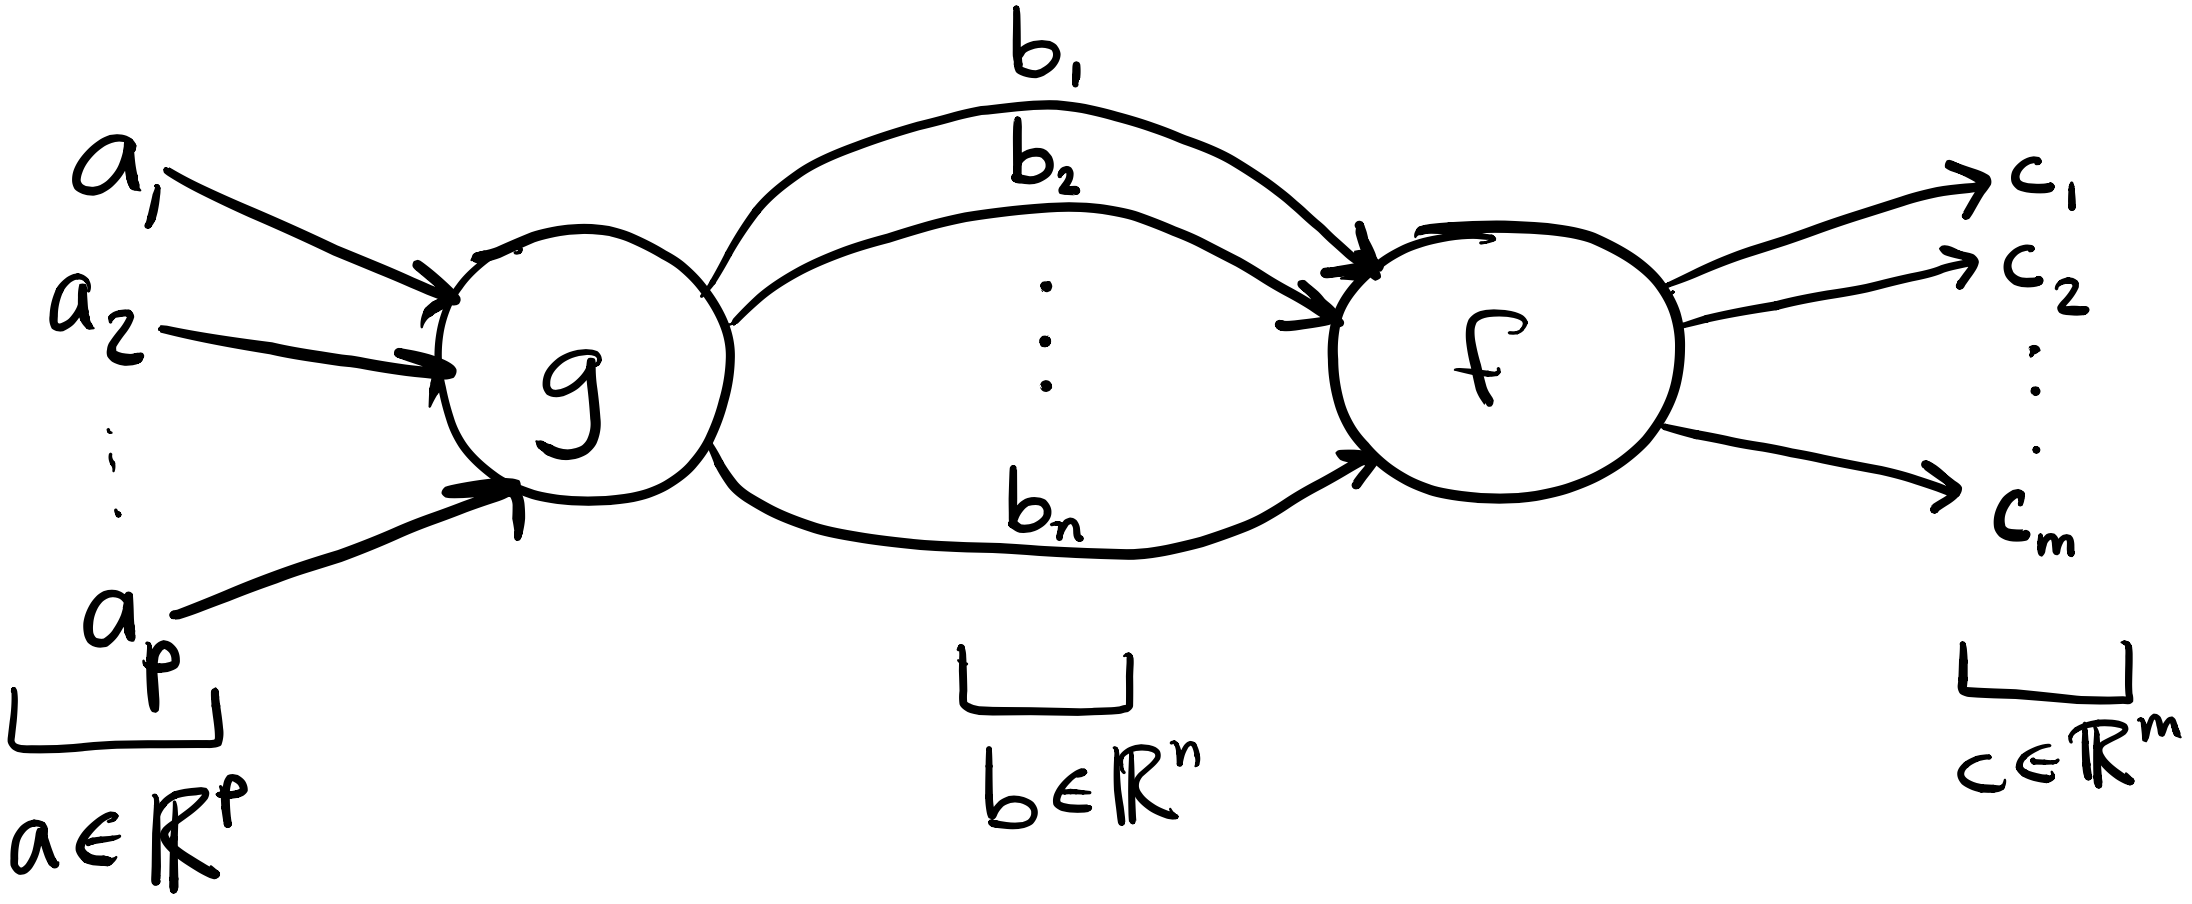
\includegraphics[width=1\columnwidth]{figures/two-fn-comp-graph-partials}
\end{figure}
\end{column}

\begin{column}{0.5\textwidth}
\begin{itemize}[<+->]
\item How does a small change in $a_j$ affect $c_i$?
\item Visualizing the \textbf{chain rule}:
\begin{itemize}[<.->]
\item We \textcolor{blue}{sum} changes induced on all paths from $a_j$ to $c_i$.
\item The change contributed by each path is the {\color{red}product} of changes on each edge along the path.
\onslide<+->{
\[
\frac{\partial c_{i}}{\partial a_{j}}={\color{blue}\sum_{k=1}^{n}}
{\color{red} \frac{\partial c_{i}}{\partial b_{k}}\frac{\partial b_{k}}{\partial a_{j}}} .
\]
}
\end{itemize} 
\end{itemize}
\end{column}
\end{columns}
\note[item]{In math, we know that $c=f(g(z))$, so that we can use chain rule. But how do we visualize chain rule on this graph?}
\note[item]{$a_j$ would affect $b_1$ to $b_n$, and each $b_k$ further affects $c_i$}.
\end{frame}

\subsection{Example Computation Graphs}
\begin{frame}{Example: Linear least squares}
\begin{itemize}
\item Hypothesis space $\left\{ f(x)=w^{T}x+b\mid w\in\reals^{d},b\in\reals\right\} $.

\item Data set $\left(x_{1},y_{1}\right),\ldots,\left(x_{n},y_{n}\right)\in\reals^{d}\times\reals$.
\item Define
\[
\ell_{i}(w,b)=\left[\left(w^{T}x_{i}+b\right)-y_{i}\right]^{2}.
\]


\pause{}
\item In SGD, in each round we choose a random training instance $i\in1,\ldots,n$
and take a gradient step
\begin{eqnarray*}
w_{j} & \gets & w_{j}-\eta\frac{\partial\ell_{i}(w,b)}{\partial w_{j}}\text{, for }j=1,\ldots,d\\
b & \gets & b-\eta\frac{\partial\ell_{i}(w,b)}{\partial b},
\end{eqnarray*}
for some step size $\eta>0$.
\item How do we calculate these partial derivatives on a computation graph?
\end{itemize}
\end{frame}
%
\begin{frame}{Computation graph and intermediate variables}
\begin{itemize}
\item For a training point $\left(x,y\right)$, the loss is
\[
\ell(w,b)=\left[\left(w^{T}x+b\right)-y\right]^{2}.
\]
\pause
\item Let's break this down into intermediate computations:
\begin{columns}[t]

\column{.35\textwidth}

\begin{eqnarray*}
\text{(prediction) }\hat{y} & = & \sum_{j=1}^{d}w_{j}x_{j}+b\\
\pause\text{(residual) }r & = & y-\hat{y}\\
\pause\text{(loss) }\ell & = & r^{2}
\end{eqnarray*}


\pause{}

\column{.65\textwidth}
\begin{center}
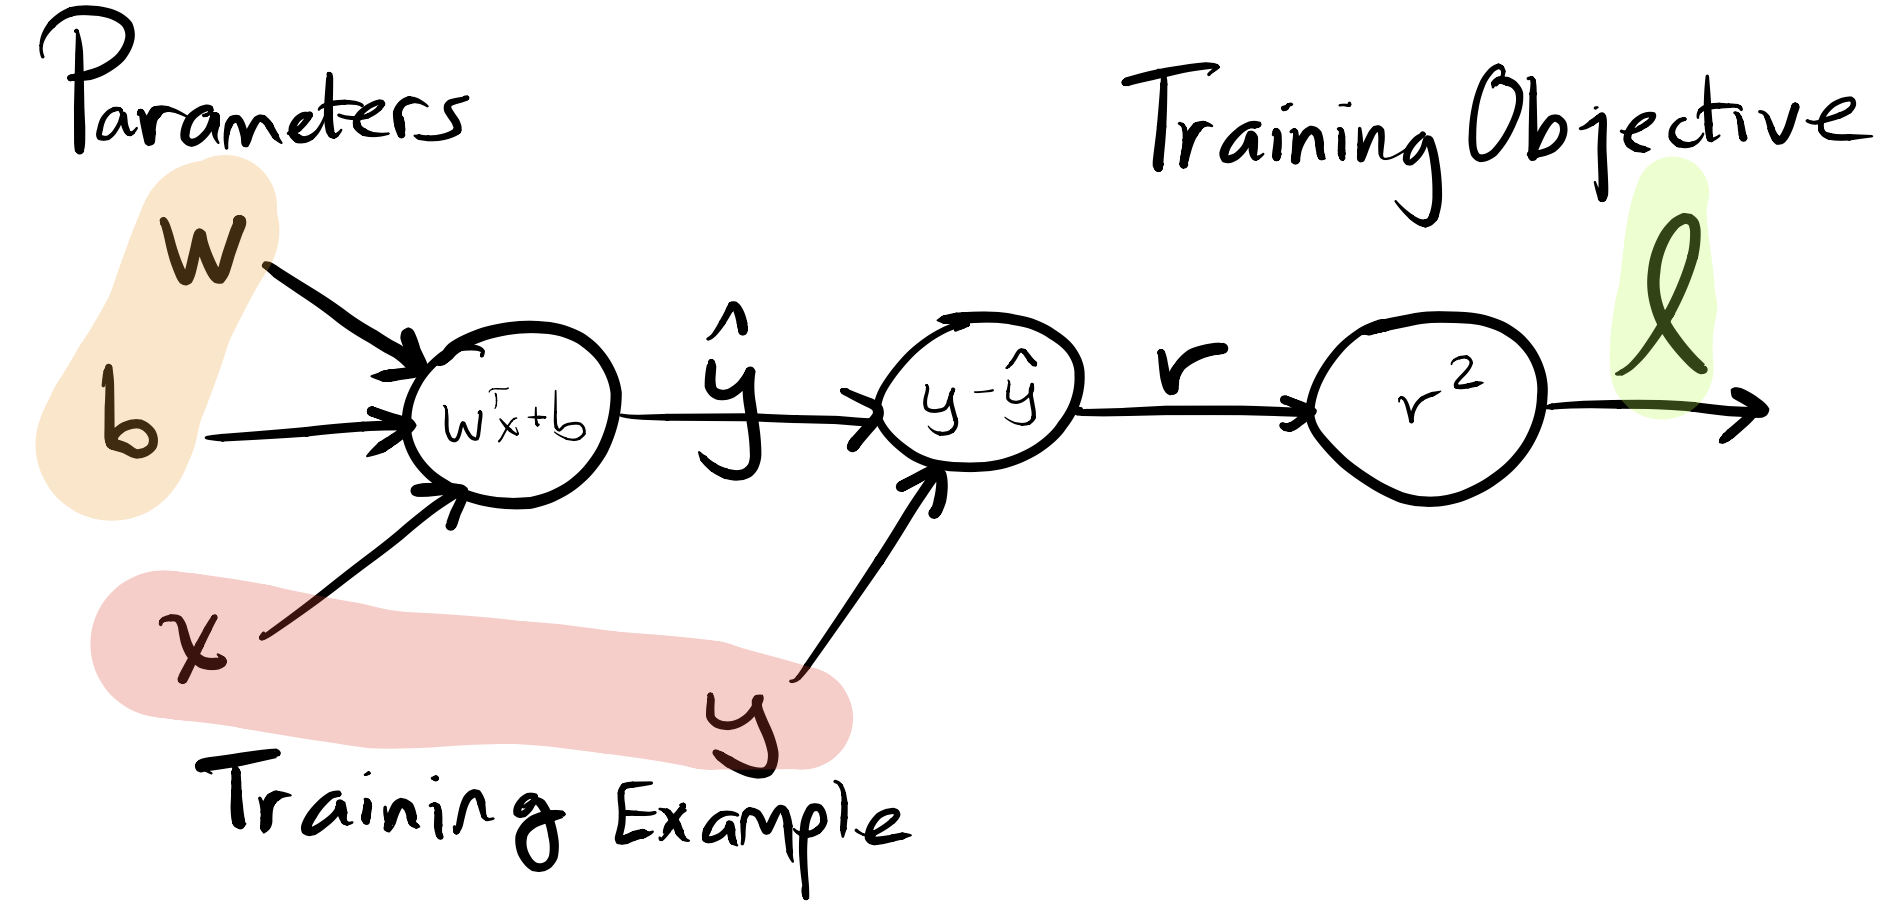
\includegraphics[height=0.45\textheight]{figures/linear-sqr-loss-comp-graph-labels}
\par\end{center}

\end{columns}

\end{itemize}
\end{frame}
%
\begin{frame}{Partial derivatives on computation graph}
\begin{itemize}
\item We'll work our way from the output $\ell$ back to the parameters
$w$ and $b$, reusing previous computations as much as possible:
\begin{columns}[c]

\column{.45\textwidth}

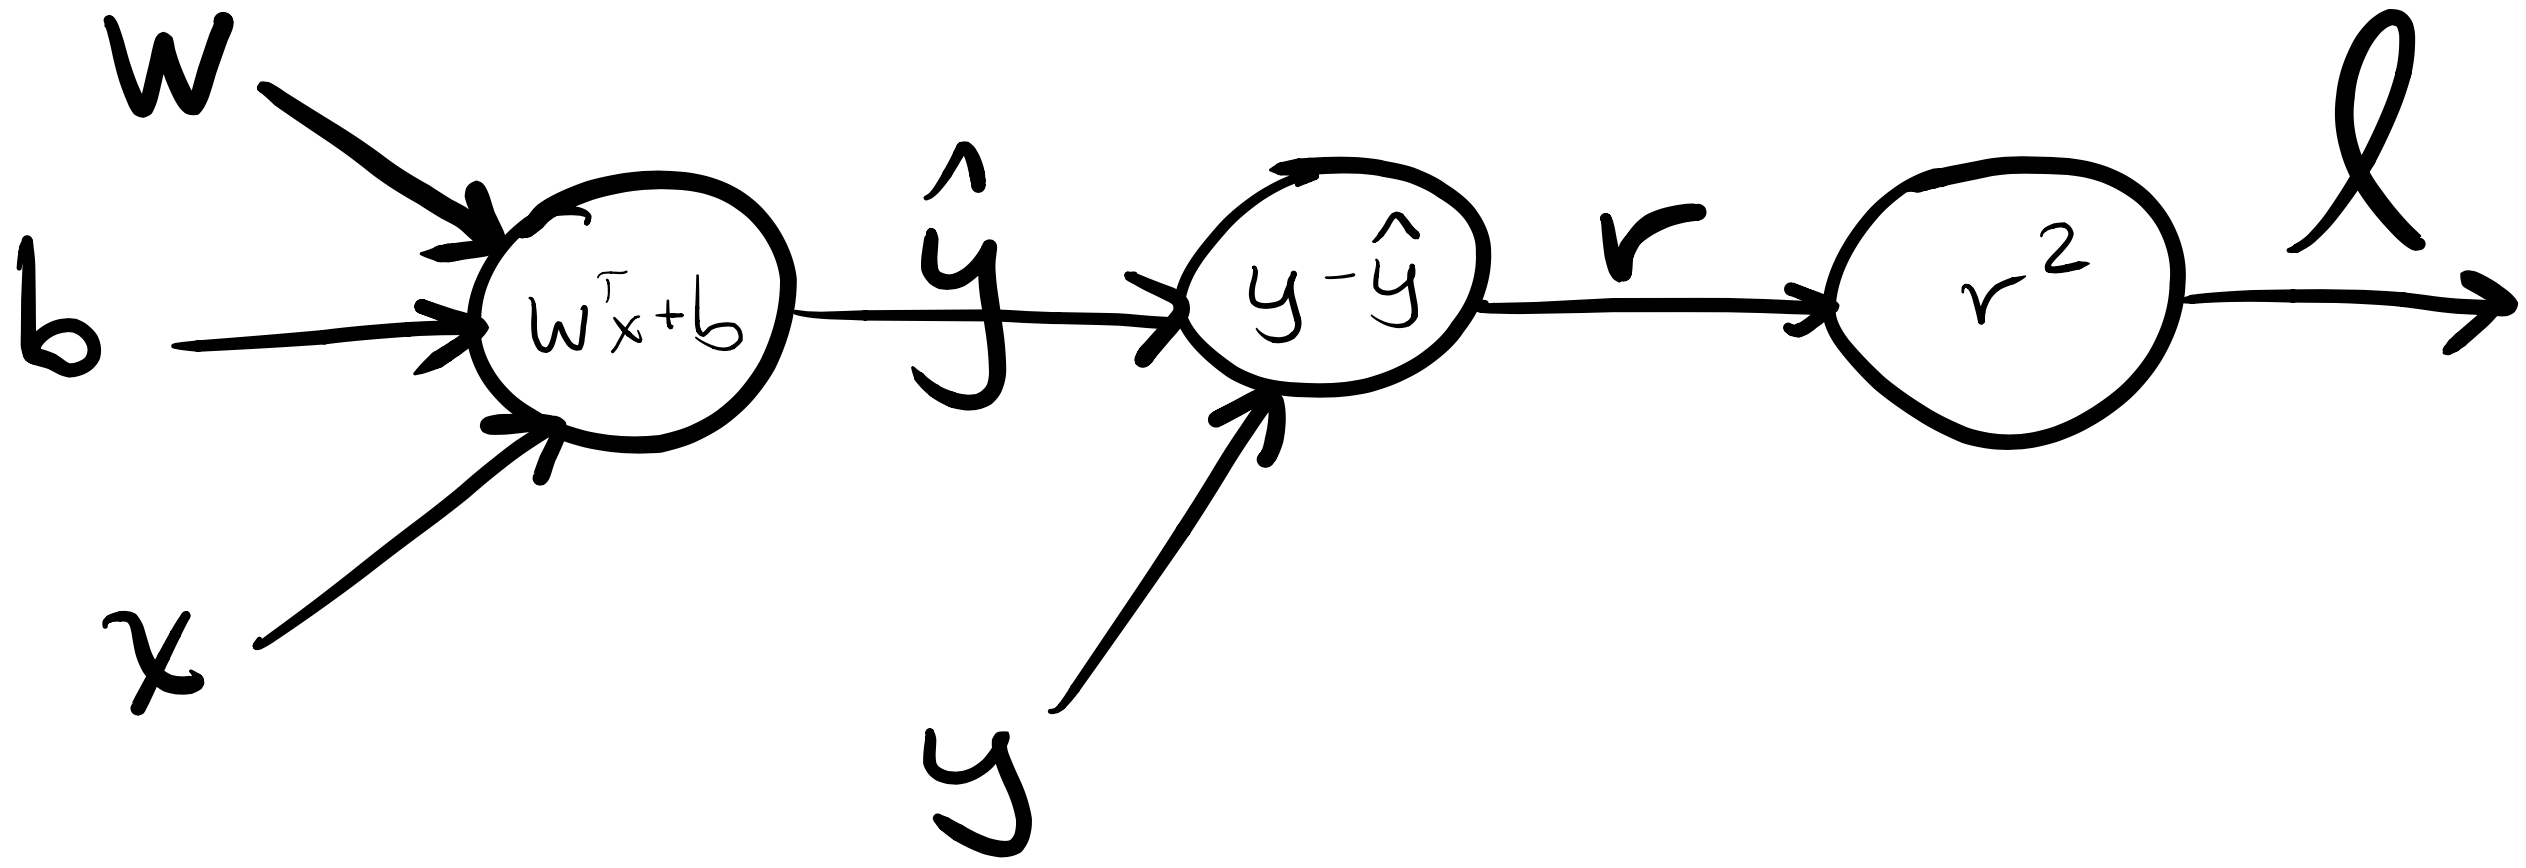
\includegraphics[width=1\columnwidth]{figures/linear-sqr-loss-comp-graph}

\pause{}

\column{.45\textwidth}

\begin{eqnarray*}
\frac{\partial\ell}{\partial r} & = & \pause2r\\
\frac{\partial\ell}{\partial\hat{y}} & = & \pause\frac{\partial\ell}{\partial r}\frac{\partial r}{\partial\hat{y}}=\left(2r\right)(-1)=-2r\\
\frac{\partial\ell}{\partial b} & = & \pause\frac{\partial\ell}{\partial\hat{y}}\frac{\partial\hat{y}}{\partial b}=\left(-2r\right)(1)=-2r\\
\frac{\partial\ell}{\partial w_{j}} & = & \pause\frac{\partial\ell}{\partial\hat{y}}\frac{\partial\hat{y}}{\partial w_{j}}=\left(-2r\right)x_{j}=-2rx_{j}
\end{eqnarray*}

\end{columns}

\end{itemize}
\note[item]{Notice that in each step we can use previous results.}
\end{frame}

\begin{frame}{Example: Ridge Regression}
\begin{itemize}
\item For training point $\left(x,y\right)$, the $\ell_{2}$-regularized
objective function is 
\[
J(w,b)=\left[\left(w^{T}x+b\right)-y\right]^{2}+\lambda w^{T}w.
\]
\item Let's break this down into some intermediate computations:
\begin{columns}[t]

\column{.35\textwidth}

\begin{eqnarray*}
\text{(prediction) }\hat{y} & = & \sum_{j=1}^{d}w_{j}x_{j}+b\\
\text{(residual) }r & = & y-\hat{y}\\
\text{(loss) }\ell & = & r^{2}\\
\pause\text{(regularization) }R & = & \lambda w^{T}w\\
\text{(objective) }J & = & \ell+R
\end{eqnarray*}


\pause{}

\column{.65\textwidth}
\begin{center}
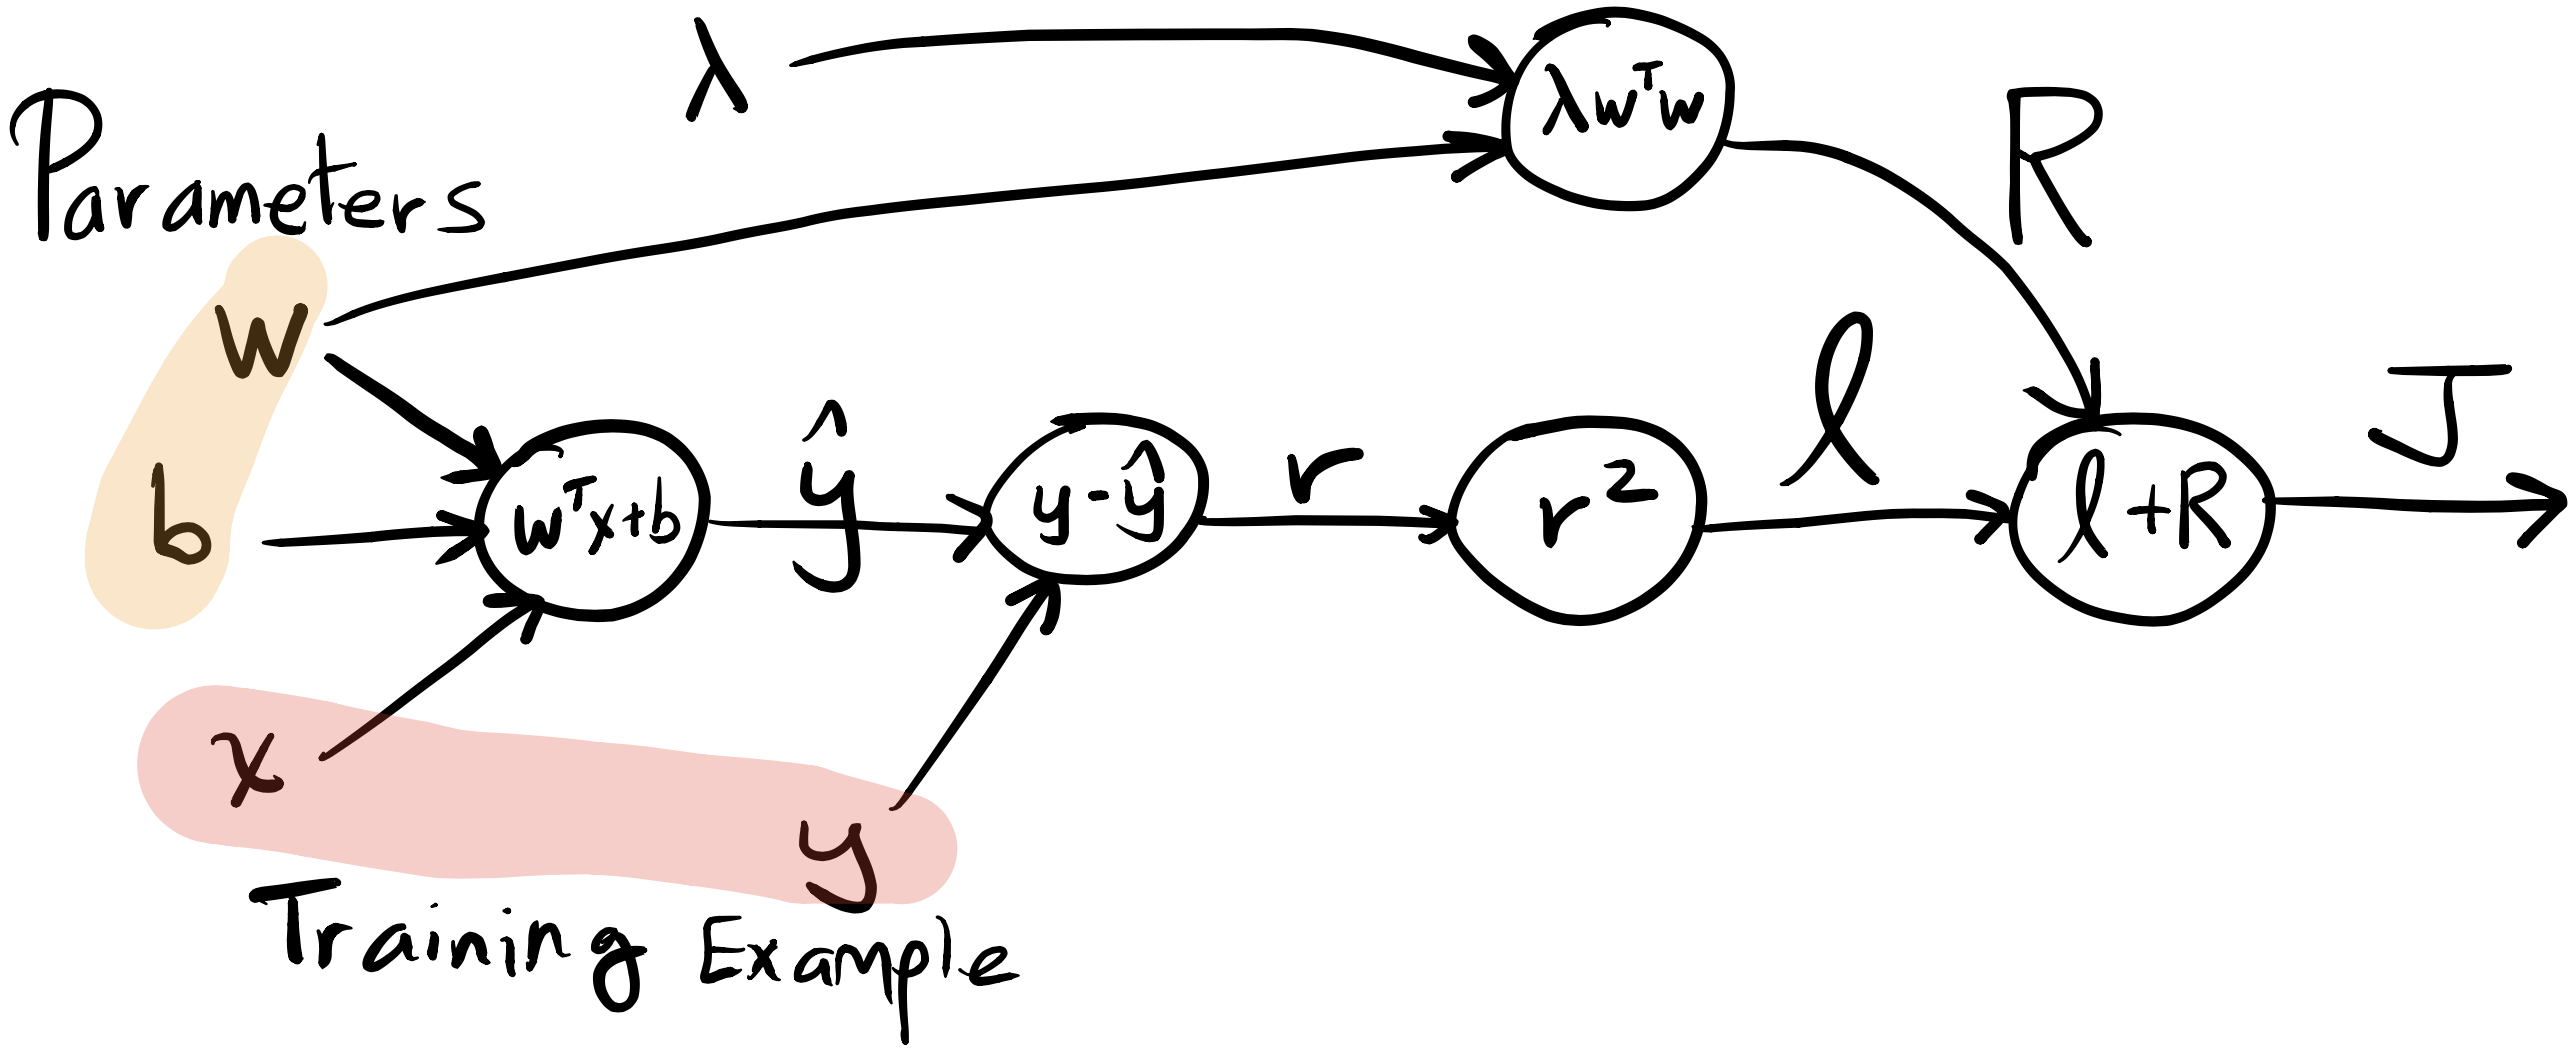
\includegraphics[height=0.45\textheight]{figures/ridge-regression-comp-graph-labels}
\par\end{center}

\end{columns}

\end{itemize}
\end{frame}

\begin{frame}{Partial Derivatives on Computation Graph}
\begin{itemize}
\item We'll work our way from graph output $\ell$ back to the parameters
$w$ and $b$:
\begin{columns}[c]

\column{.55\textwidth}

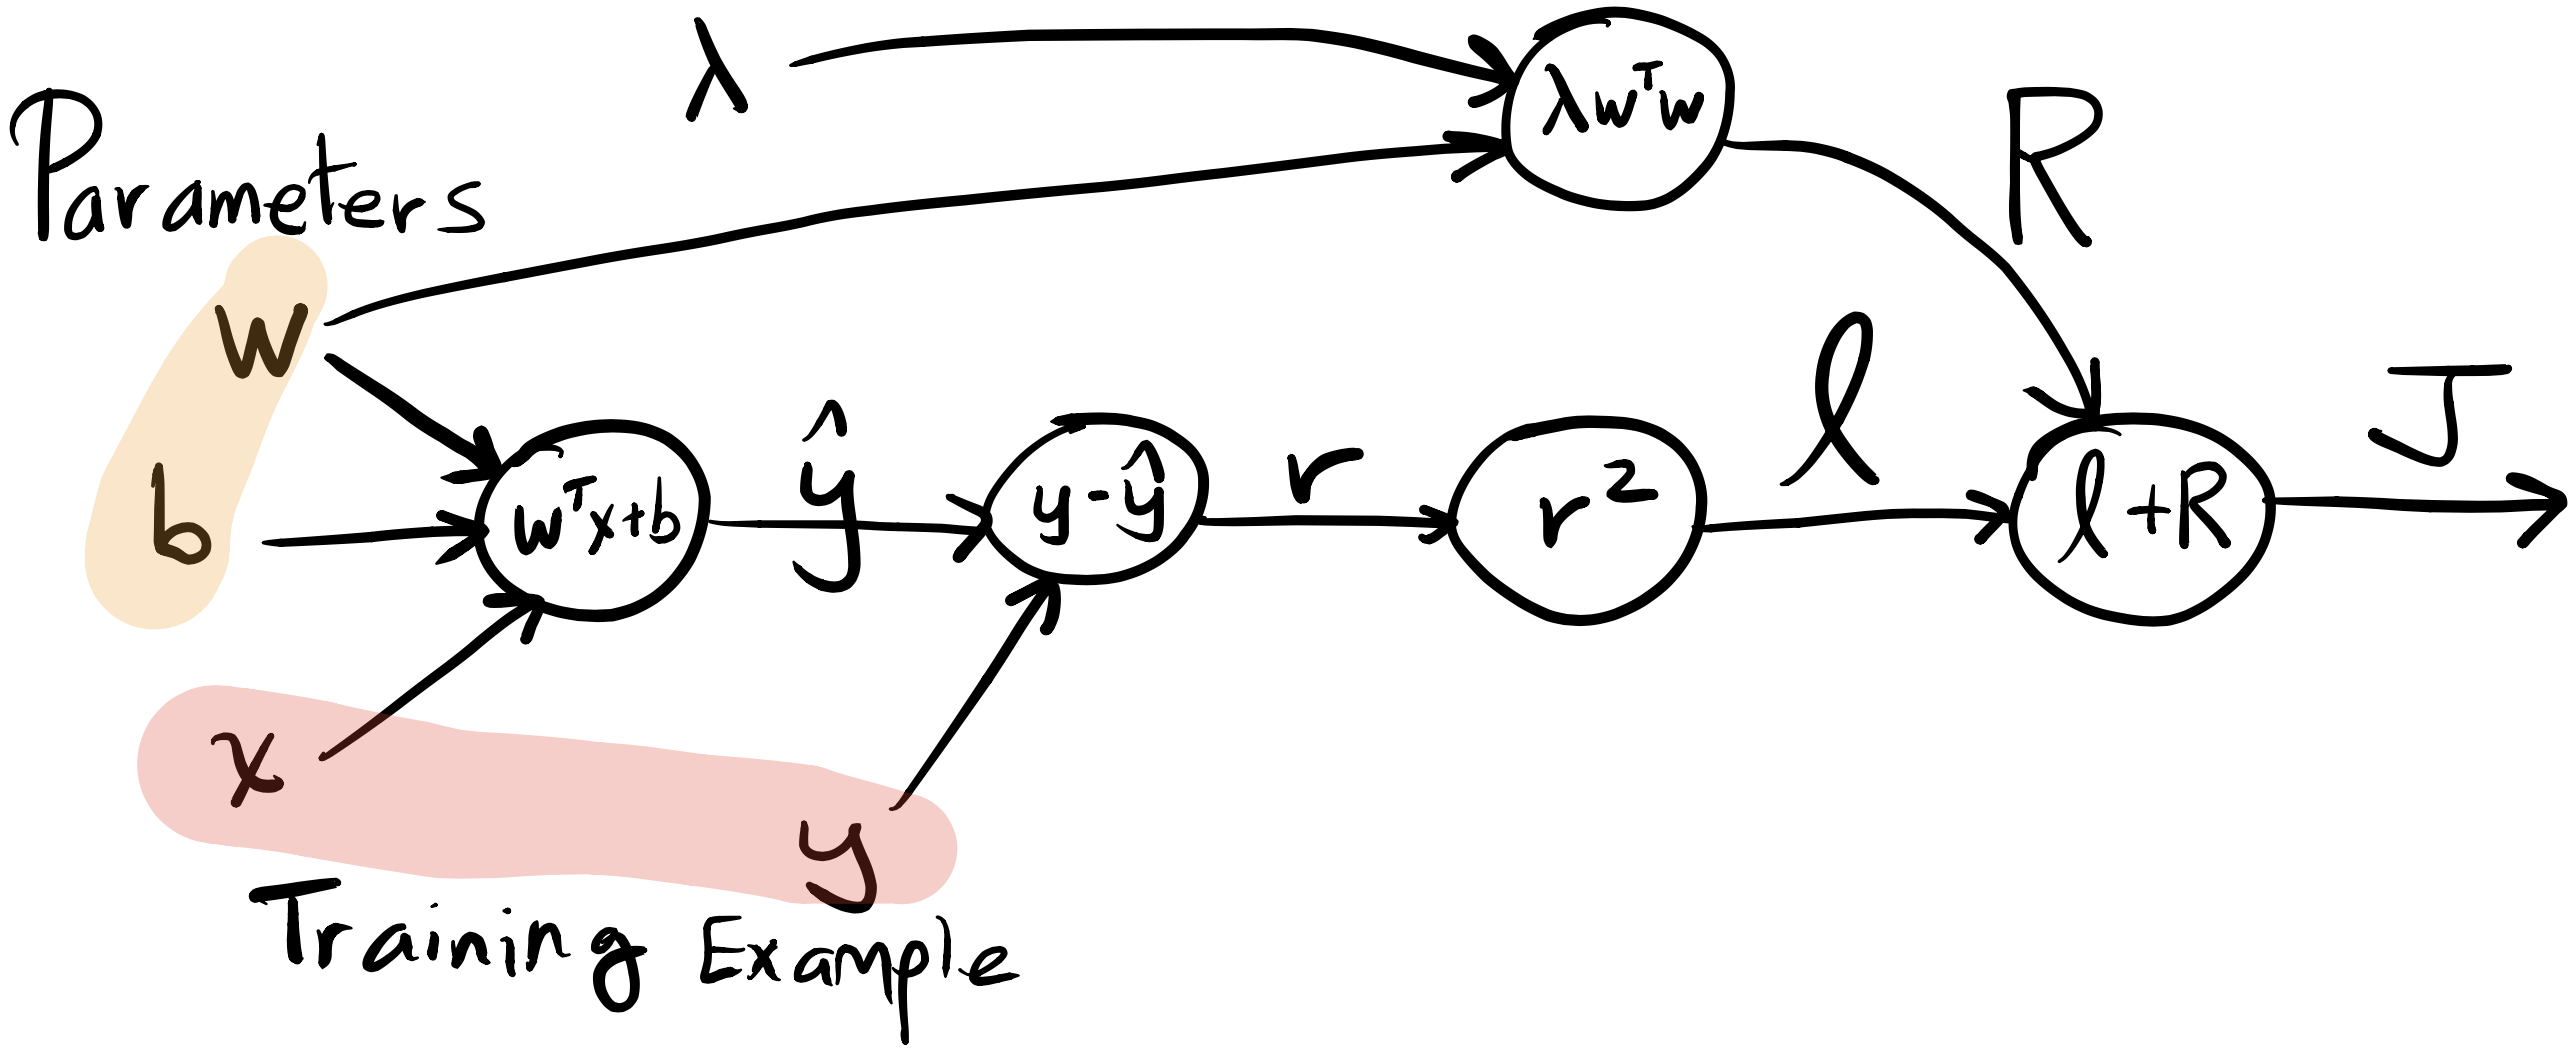
\includegraphics[width=1\columnwidth]{figures/ridge-regression-comp-graph-labels}


\column{.45\textwidth}

\begin{eqnarray*}
\frac{\partial J}{\partial\ell} & = & \frac{\partial J}{\partial R}=1\\
\frac{\partial J}{\partial\hat{y}} & = & \frac{\partial J}{\partial\ell}\frac{\partial\ell}{\partial r}\frac{\partial r}{\partial\hat{y}}=\left(1\right)(2r)\left(-1\right)=-2r\\
\frac{\partial J}{\partial b} & = & \frac{\partial J}{\partial\hat{y}}\frac{\partial\hat{y}}{\partial b}=\left(-2r\right)\left(1\right)=-2r\\
\frac{\partial J}{\partial w_{j}} & = & \text{\think{Exercise}} 
\end{eqnarray*}

\end{columns}

\end{itemize}
\end{frame}
%
%\begin{frame}{Handling Nodes with Multiple Children}
%\begin{itemize}
%\item Consider $a\mapsto J=h(f(a),g(a))$.
%\end{itemize}
%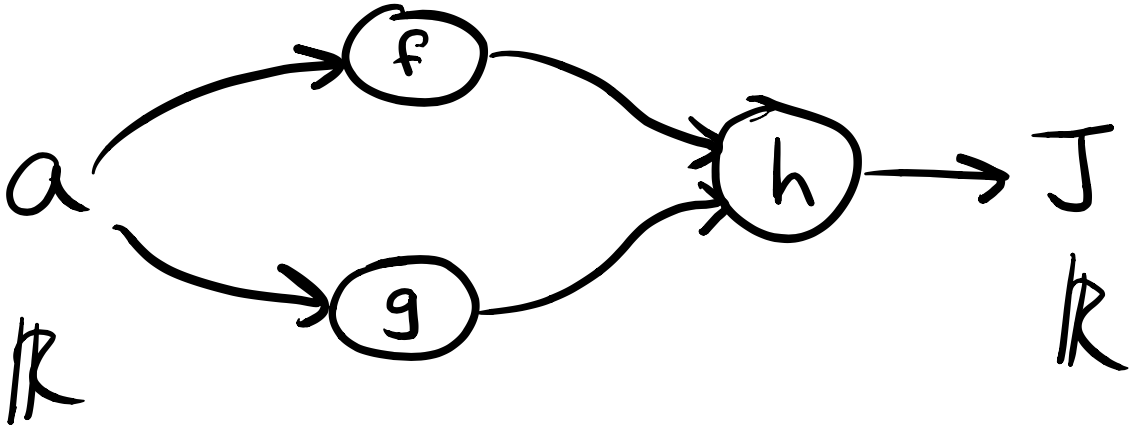
\includegraphics[height=0.3\textheight]{figures/split-output}
%\begin{itemize}
%\item It's helpful to think about having two independent copies of $a$,
%call them $a^{(1)}$ and $a^{(2)}$...
%\end{itemize}
%\end{frame}
%%
%\begin{frame}{Handling Nodes with Multiple Children}
%\begin{columns}[c]
%
%\column{.45\textwidth}
%
%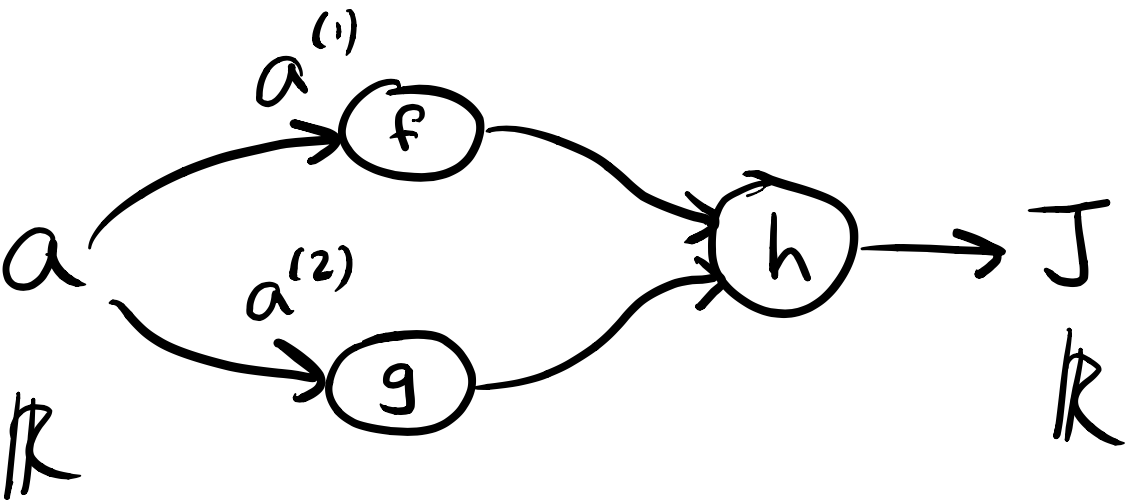
\includegraphics[width=1\columnwidth]{figures/split-output-2copies}
%
%\pause{}
%
%\column{.45\textwidth}
%
%\begin{eqnarray*}
%\frac{\partial J}{\partial a} & = & \pause\frac{\partial J}{\partial a^{(1)}}\frac{\partial a^{(1)}}{\partial a}+\frac{\partial J}{\partial a^{(2)}}\frac{\partial a^{(2)}}{\partial a}\\
% & = & \pause\frac{\partial J}{\partial a^{(1)}}+\frac{\partial J}{\partial a^{(2)}}
%\end{eqnarray*}
%
%\end{columns}
%
%\begin{itemize}
%\item Derivative w.r.t. $a$ is the sum of derivatives w.r.t. each copy
%of $a$.
%\end{itemize}
%\end{frame}
%%
%\begin{frame}{Partial Derivatives on Computation Graph}
%\begin{itemize}
%\item We'll work our way from graph output $\ell$ back to the parameters
%$w$ and $b$:
%\begin{columns}[c]
%
%\column{.45\textwidth}
%
%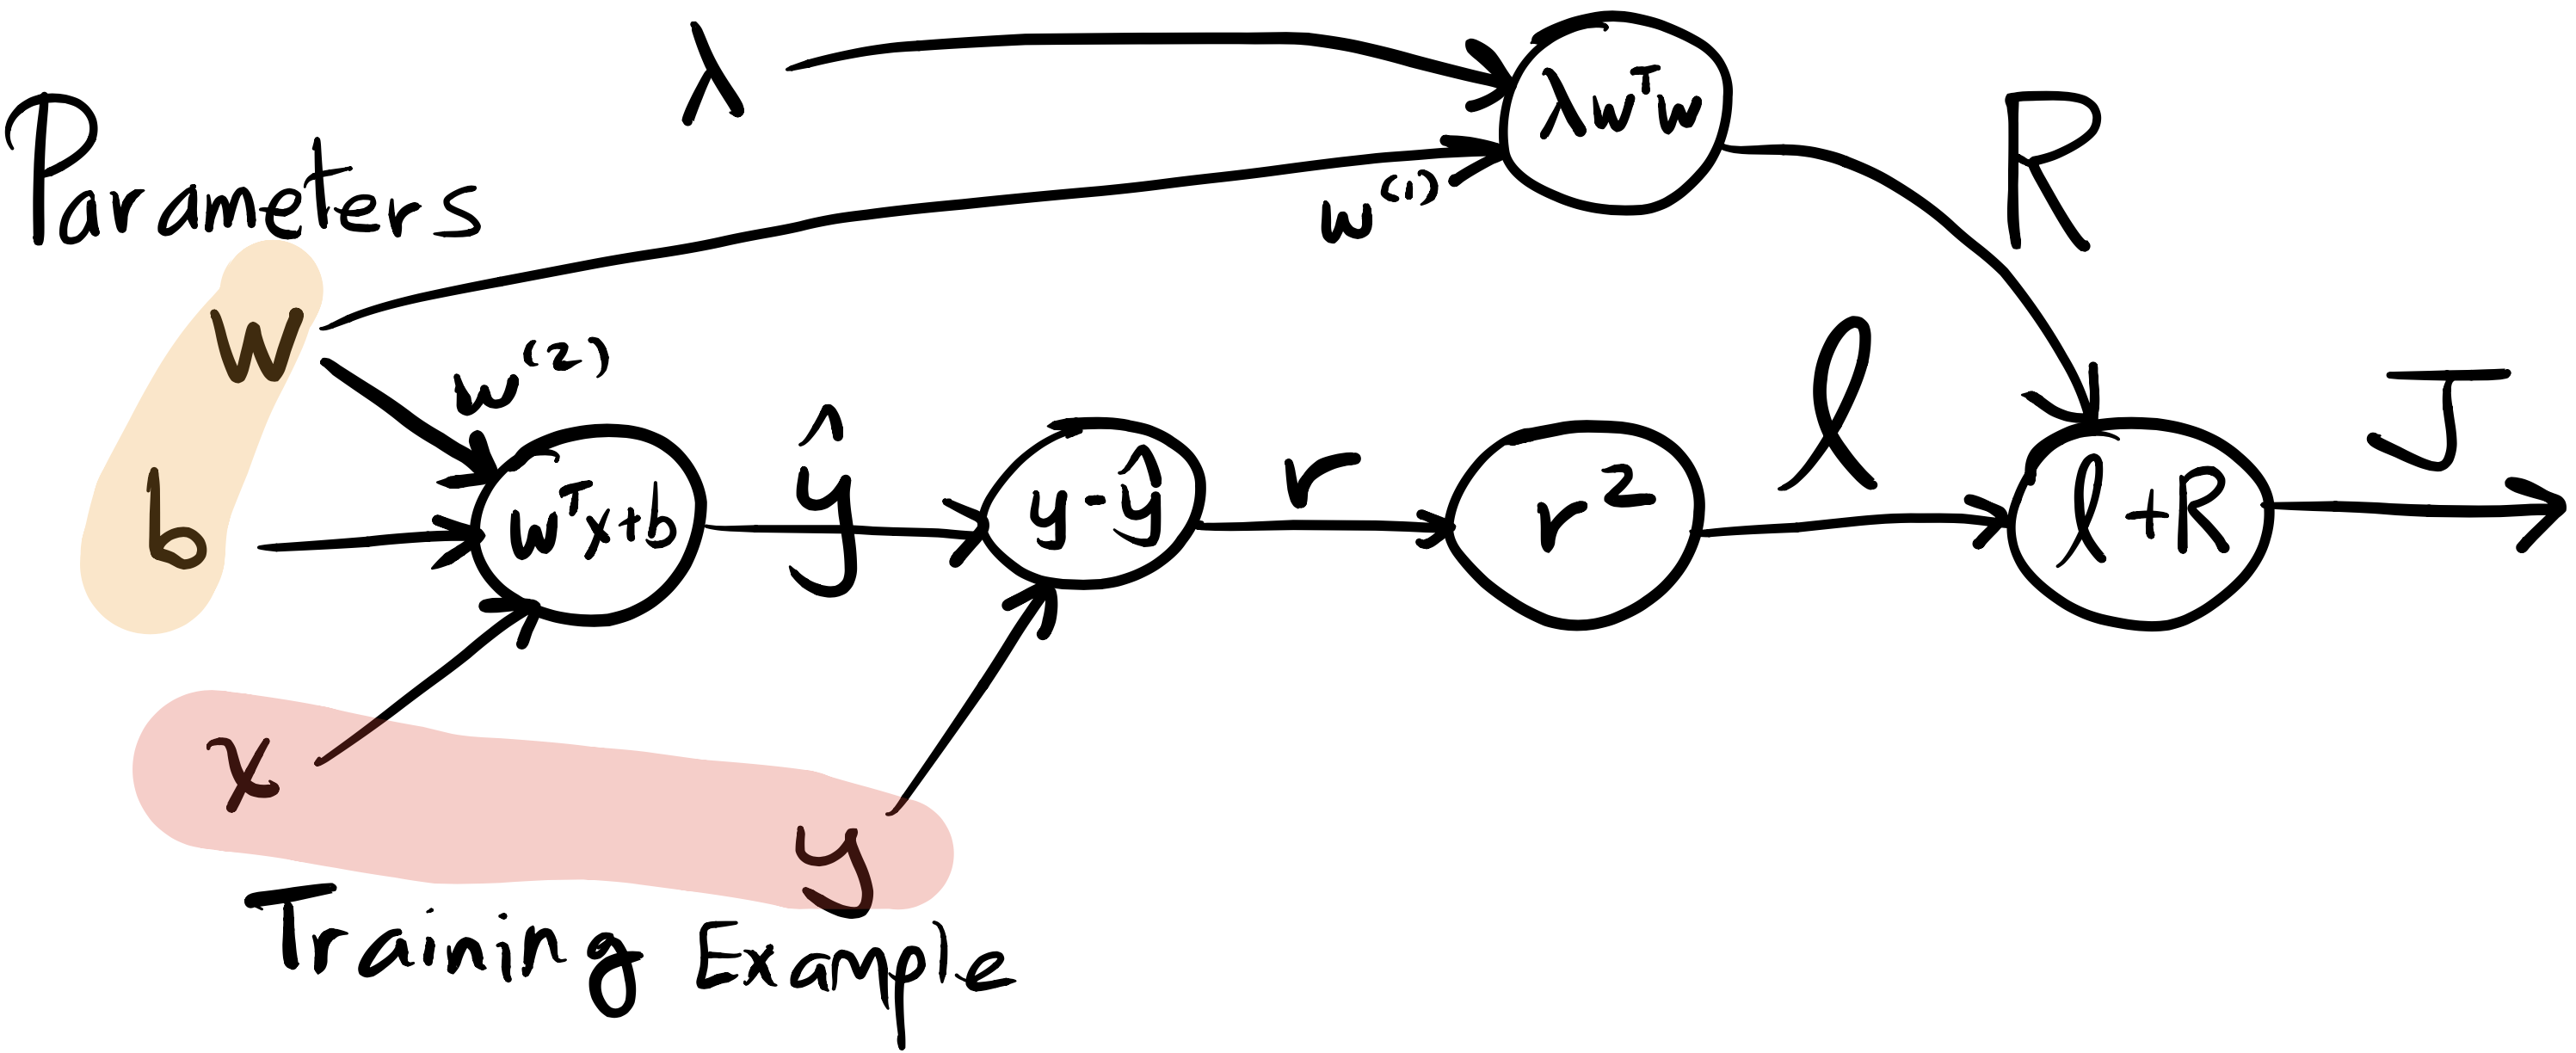
\includegraphics[width=1\columnwidth]{figures/ridge-regression-comp-graph-labels-2copies}
%
%\pause{}
%
%\column{.45\textwidth}
%
%\begin{eqnarray*}
%\frac{\partial J}{\partial\hat{y}} & = & \frac{\partial J}{\partial\ell}\frac{\partial\ell}{\partial r}\frac{\partial r}{\partial\hat{y}}=\left(1\right)(2r)\left(-1\right)=-2r\\
%\frac{\partial J}{\partial w_{j}^{(2)}} & = & \pause\frac{\partial J}{\partial\hat{y}}\frac{\partial\hat{y}}{\partial w_{j}^{(2)}}=\frac{\partial J}{\partial\hat{y}}x_{j}\\
%\frac{\partial J}{\partial w_{j}^{(1)}} & = & \pause\frac{\partial J}{\partial R}\frac{\partial R}{\partial w_{j}^{(1)}}=\left(1\right)\left(2\lambda w_{j}^{(1)}\right)\\
%\frac{\partial J}{\partial w_{j}} & = & \pause\frac{\partial J}{\partial w_{j}^{(1)}}+\frac{\partial J}{\partial w_{j}^{(2)}}
%\end{eqnarray*}
%
%\end{columns}
%
%\end{itemize}
%\end{frame}

\subsection{General Backpropagation}
\begin{frame}
{Backpropagation: Overview}
\begin{itemize}
\item \textbf{Learning}: run gradient descent to find the parameters that minimize our objective $J$.
\item Backpropagation: we compute the gradient w.r.t. each (trainable) parameter $\frac{\partial J}{\partial \theta_i}$.
\end{itemize}

\begin{columns}
\begin{column}{0.45\textwidth}
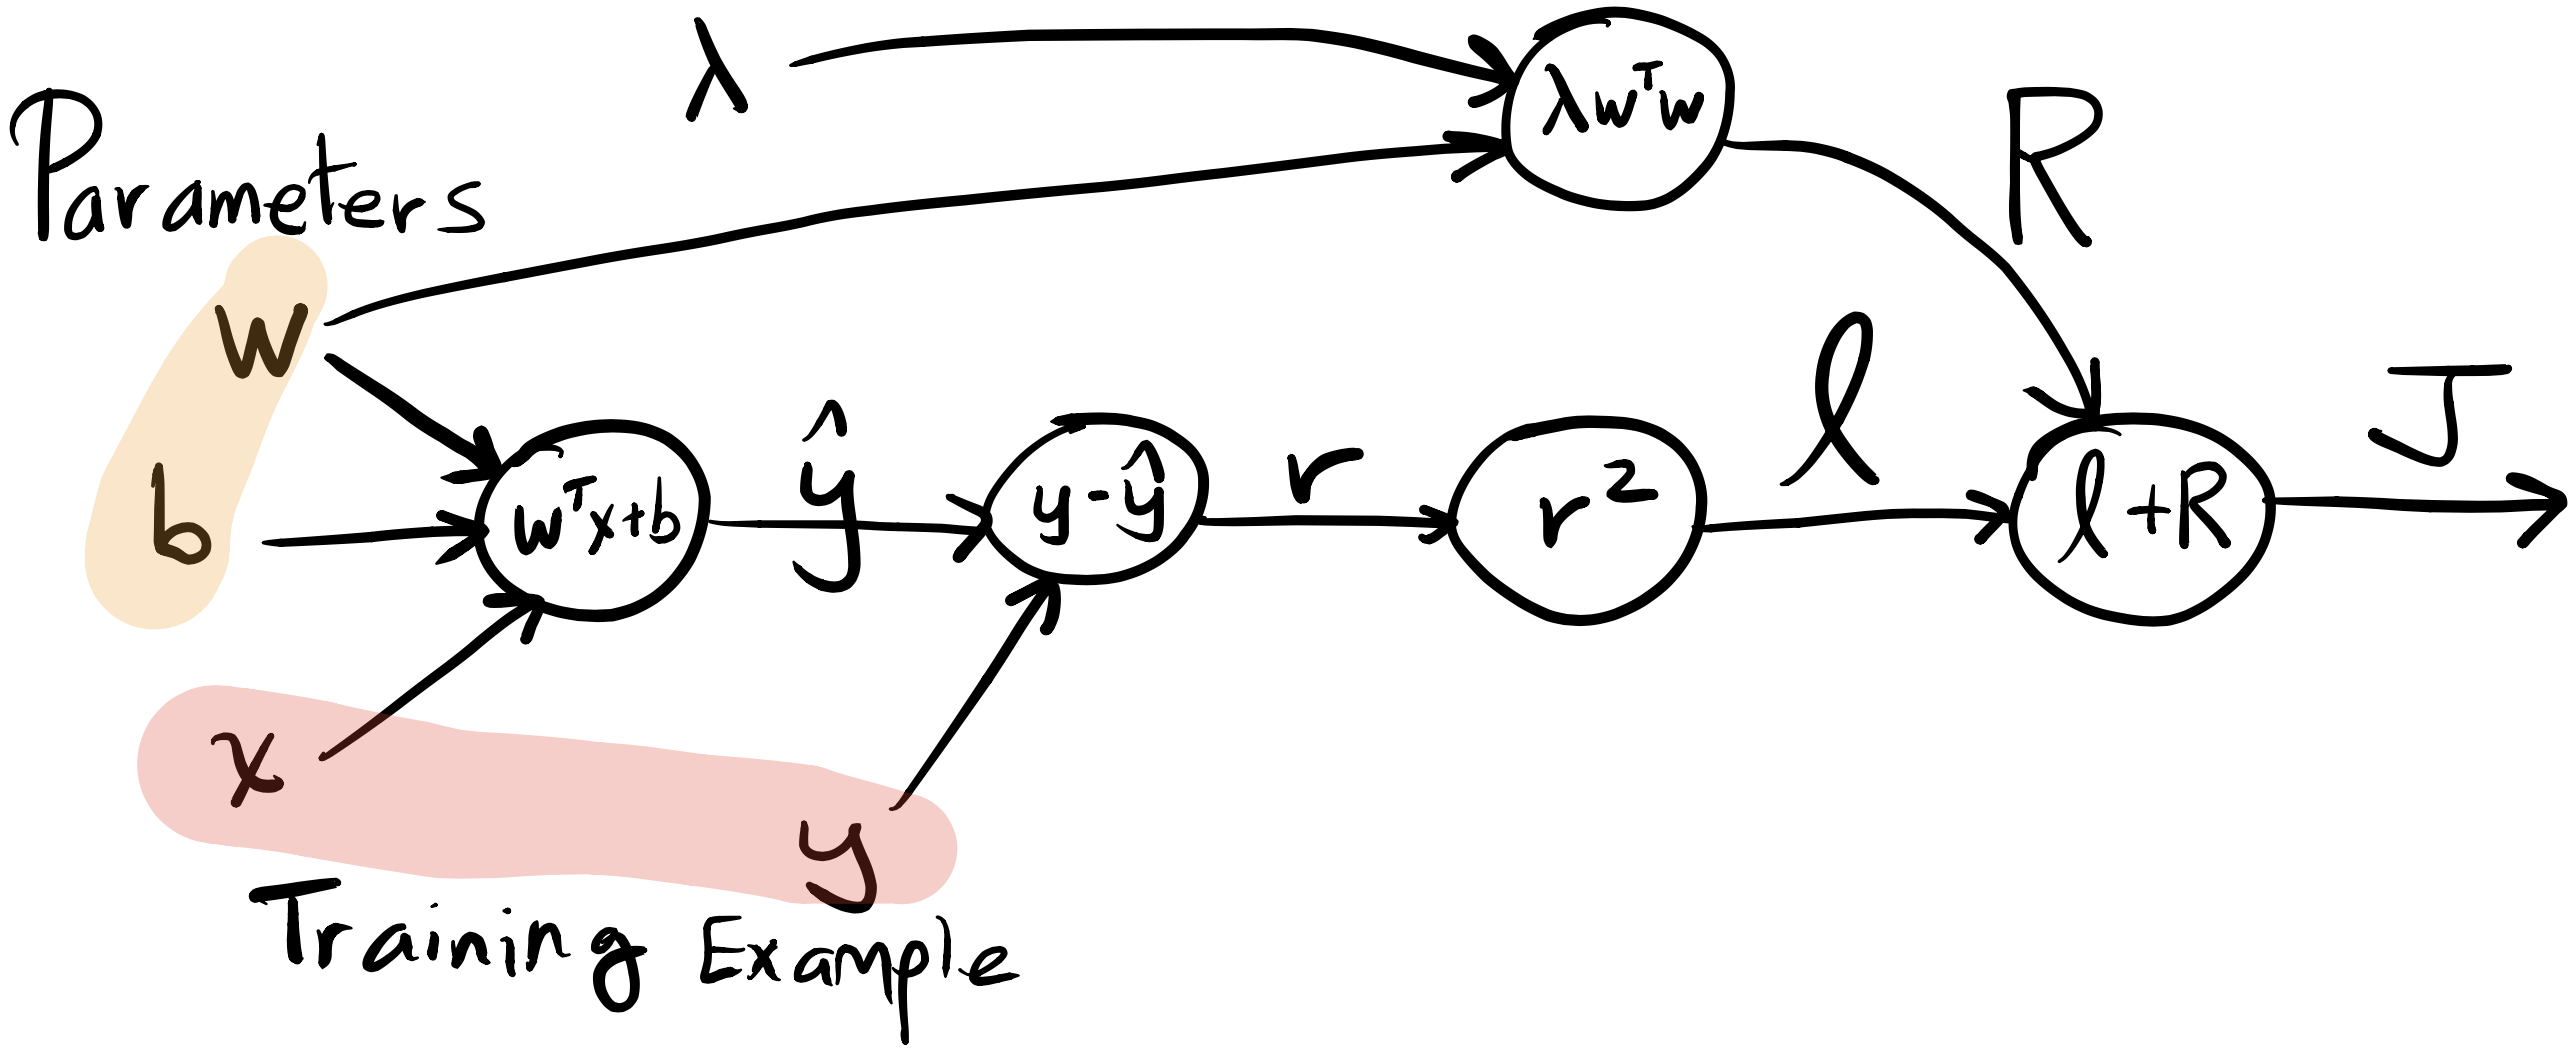
\includegraphics[width=1\columnwidth]{figures/ridge-regression-comp-graph-labels}
\end{column}
\begin{column}{0.55\textwidth}
\begin{description}[Backward pass]
\item[Forward pass] Compute intermediate function values, \ie output of each node
\item[Backward pass] Compute the partial derivative of $J$ w.r.t. all intermediate variables and the model parameters
\end{description}
\begin{simpleblock}{How do we minimize computation?}
\pause
\begin{itemize}
    \item Path sharing: each node \emph{caches intermediate results}: we don't need to compute them over and over again
\item An example of dynamic programming
\end{itemize}
\end{simpleblock}
\end{column}
\end{columns}
\end{frame}

\begin{frame}
{Forward pass}
\begin{itemize}
\item Order nodes by \textbf{topological sort} (every node appears before its children)
\item For each node, compute the output given the input (output of its parents).
\item Forward at intermediate node $f_i$ and $f_j$:
\end{itemize}
\begin{center}
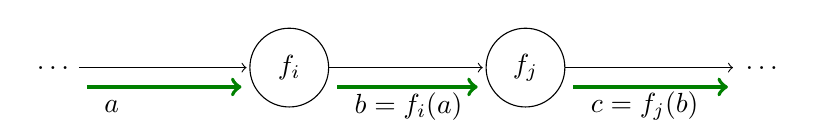
\begin{tikzpicture}[shorten >=1pt]
      	\tikzstyle{unit}=[draw,shape=circle,minimum size =1cm]

		\node (start) at (0,1){$\ldots$};
       	\node[unit](i) at (3,1){$f_i$};
        	\node[unit](j) at (6,1){$f_j$};
        	\node (end) at (9,1){$\ldots$};

        	\draw[->] (i) -- (j);
        	\draw[->] (start) -- (i);
        	\draw[->] (j) -- (end);
		
		\begin{scope}[transform canvas={yshift=-.7em}]
		\draw [->, Green, line width=0.05cm, shorten <=1mm, shorten >=1mm] (start) -- node {} (i);
  		\draw [->, Green, line width=0.05cm, shorten <=1mm, shorten >=1mm] (i) -- node {} (j);
  		\draw [->, Green, line width=0.05cm, shorten <=1mm, shorten >=1mm] (j) -- node {} (end);
		\end{scope}
		
		\begin{scope}[transform canvas={yshift=-1.4em}]
		\node (i-in) [right=0.2cm of start] {$a$};
		\node (j-in) [right=0.2cm of i] {$b=f_i(a)$};
		\node (j-out) [right=0.2cm of j] {$c=f_j(b)$};
		\end{scope}
\end{tikzpicture}
\end{center}
\end{frame}

\begin{frame}
{Backward pass}
\begin{itemize}
\item Order nodes in \textbf{reverse topological order} (every node appears after its children)
\item For each node, compute the partial derivative of its output w.r.t. its input, multiplied by the partial derivative of its children (chain rule)
\item Backward pass at intermediate node $f_i$:
\end{itemize}
\begin{center}
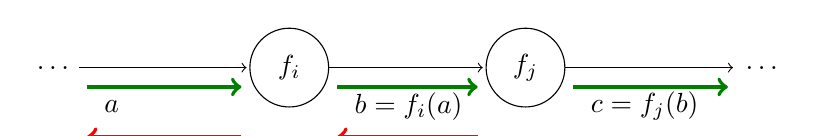
\begin{tikzpicture}[shorten >=1pt]
      	\tikzstyle{unit}=[draw,shape=circle,minimum size =1cm]

		\node (start) at (0,1){$\ldots$};
       	\node[unit](i) at (3,1){$f_i$};
        	\node[unit](j) at (6,1){$f_j$};
        	\node (end) at (9,1){$\ldots$};

        	\draw[->] (i) -- (j);
        	\draw[->] (start) -- (i);
        	\draw[->] (j) -- (end);
		
		\begin{scope}[transform canvas={yshift=-.7em}]
		\draw [->, Green, line width=0.05cm, shorten <=1mm, shorten >=1mm] (start) -- node {} (i);
  		\draw [->, Green, line width=0.05cm, shorten <=1mm, shorten >=1mm] (i) -- node {} (j);
  		\draw [->, Green, line width=0.05cm, shorten <=1mm, shorten >=1mm] (j) -- node {} (end);
		\end{scope}
		
		\begin{scope}[transform canvas={yshift=-1.4em}]
		\node (i-in) [right=0.2cm of start] {$a$};
		\node (j-in) [right=0.2cm of i] {$b=f_i(a)$};
		\node (j-out) [right=0.2cm of j] {$c=f_j(b)$};
		\end{scope}
		
		\begin{scope}[transform canvas={yshift=-2.5em}]
		\draw [<-, red, line width=0.05cm, shorten <=1mm, shorten >=1mm] (start) -- node {} (i);
  		\draw [<-, red, line width=0.05cm, shorten <=1mm, shorten >=1mm] (i) -- node {} (j);
%  		\draw [<-, red, line width=0.05cm, shorten <=1mm, shorten >=1mm] (j) -- node {} (end);
		\end{scope}
		
		\begin{scope}[transform canvas={yshift=-3.4em}]
		\node (i-out) [left=0.2cm of i] {$g_i=g_j \cdot \frac{\partial b}{\partial a} = \frac{\partial J}{\partial a}$};
		\node (j-out) [left=0.2cm of j] {$g_j=\frac{\partial J}{\partial b}$};
		\end{scope}
\end{tikzpicture}
\end{center}
\end{frame}

\begin{frame}{Multiple children}
\begin{itemize}
\item First sum partial derivatives from all children, then multiply.
\begin{columns}[c]

\column{.45\textwidth}

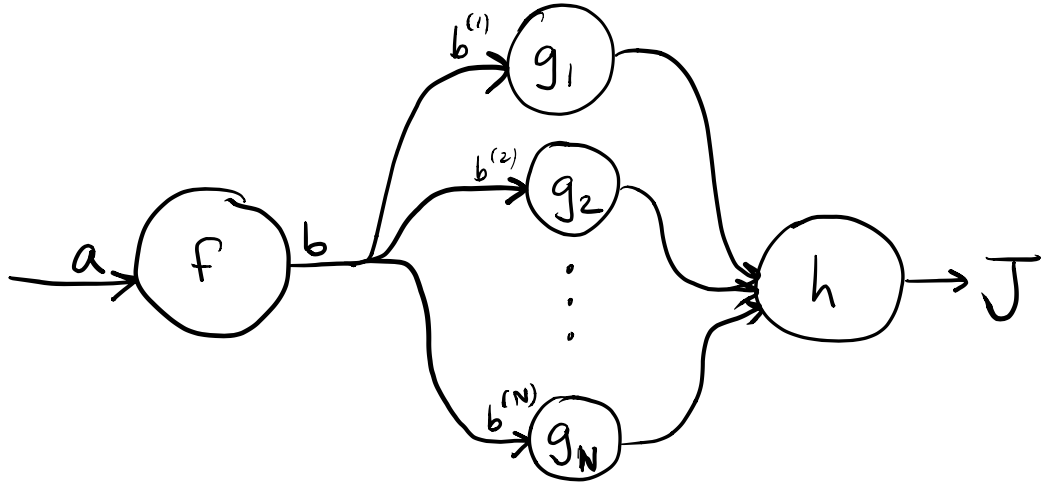
\includegraphics[width=1\columnwidth]{figures/backprop-general-node}

\pause{}

\column{.5\textwidth}
\begin{itemize}
\item Backprop for node $f$:
\item \textbf{Input}: $\frac{\partial J}{\partial b^{(1)}},\ldots,\frac{\partial J}{\partial b^{(N)}}$
\\
(Partials w.r.t. inputs to all children)
\item \textbf{Output}: 
\begin{eqnarray*}
\frac{\partial J}{\partial b} & = & \sum_{k=1}^{N}\frac{\partial J}{\partial b^{(k)}}\\
\text{ }\frac{\partial J}{\partial a} & = & \frac{\partial J}{\partial b}\frac{\partial b}{\partial a}
\end{eqnarray*}
\end{itemize}
\end{columns}

\end{itemize}
\end{frame}
%
%

\begin{frame}{Why backward?}
\begin{itemize}
    \item<+-> We can write the chain rule in different orders of computation.
    \begin{align}
    y &= y(c(b(a)))\\
    \uncover<+->{
    \frac{\partial y}{\partial a} &= \underbrace{\frac{\partial y}{\partial c}}_{D_4 \times D_3} \underbrace{\frac{\partial c}{\partial b}}_{D_3 \times D_2} \underbrace{\frac{\partial b}{\partial a}}_{D_2 \times D_1} \\
    }
    \uncover<+->{
    \text{Backward:\ \ \ } \frac{\partial y}{\partial a} &= \underbrace{\frac{\partial y}{\partial c}\frac{\partial c}{\partial b}}_{D_4 \times D_3 \cdot D_3 \times D_2 \rightarrow D_4 \times D_2}\ \underbrace{\frac{\partial b}{\partial a}}_{D_2 \times D_1} \\
    }
    \uncover<+->{
    \text{Forward:\ \ \ }\frac{\partial y}{\partial a} &= \underbrace{\frac{\partial y}{\partial c}}_{D_4 \times D_3} \underbrace{\frac{\partial c}{\partial b}\frac{\partial b}{\partial a}}_{D_3 \times D_2 \cdot D_2 \times D_1 \rightarrow D_3 \times D_1}}
    \end{align}
    
\end{itemize}
\end{frame}

\begin{frame}{Trade-offs}
\begin{itemize}
    \item<+-> The \textbf{reverse} order: The \textbf{last} dimention ($D_4$) is preserved throughout propagation.
    \item<+-> The \textbf{forward} order: The \textbf{first} dimension ($D_1$) is preserved throughout propagation.
    \item<+->  Reverse mode automatic differentiation (backprop) is faster since we have a scalar output and a vector input, and it works well on most neural networks.
    \item<+->  Forward mode automatic differentiation could be faster if we have a scalar input and a vector output (less memory).
    \item<+->  Optimal ordering = matrix chain ordering problem. Dynamic programming solution.
\end{itemize}
\end{frame}

\begin{frame}
{Non-convex optimization}
\begin{figure}
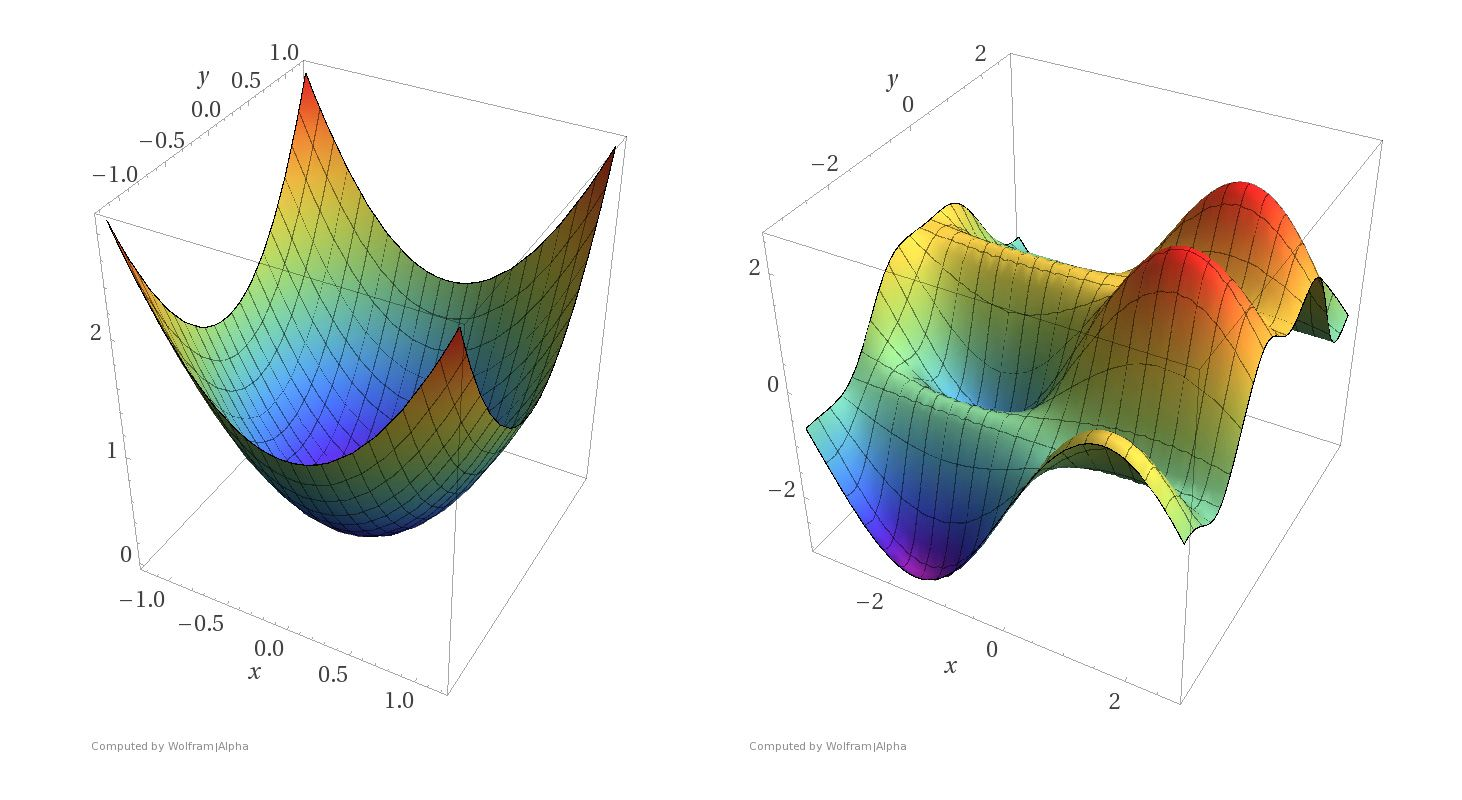
\includegraphics[height=0.7\textheight]{figures/convex_cost_function}
\end{figure}
\begin{itemize}
\item Left: convex loss function. Right: non-convex loss function.
\end{itemize}
\end{frame}

\begin{frame}
{Non-convex optimization: challenges}
\begin{columns}
\begin{column}{0.6\textwidth}
\begin{itemize}
\item What if we converge to a bad local minimum?
\uncover<+->{
\begin{itemize}
\item Rerun with a different initialization
\end{itemize}
}
\uncover<+->{
\item Hit a saddle point 
\begin{itemize}
\item Doesn't often happen with SGD 
\item Second partial derivative test
\end{itemize}
}
\uncover<+->{
\item Flat region: low gradient magnitude
\begin{itemize}
\item Possible solution: use ReLU instead of sigmoid 
\end{itemize}
}
\uncover<+->{
\item High curvature: large gradient magnitude
\begin{itemize}
\item Possible solutions: Gradient clipping, adaptive step sizes
\end{itemize}
}
\end{itemize}
\end{column}
\begin{column}{0.4\textwidth}
\begin{figure}
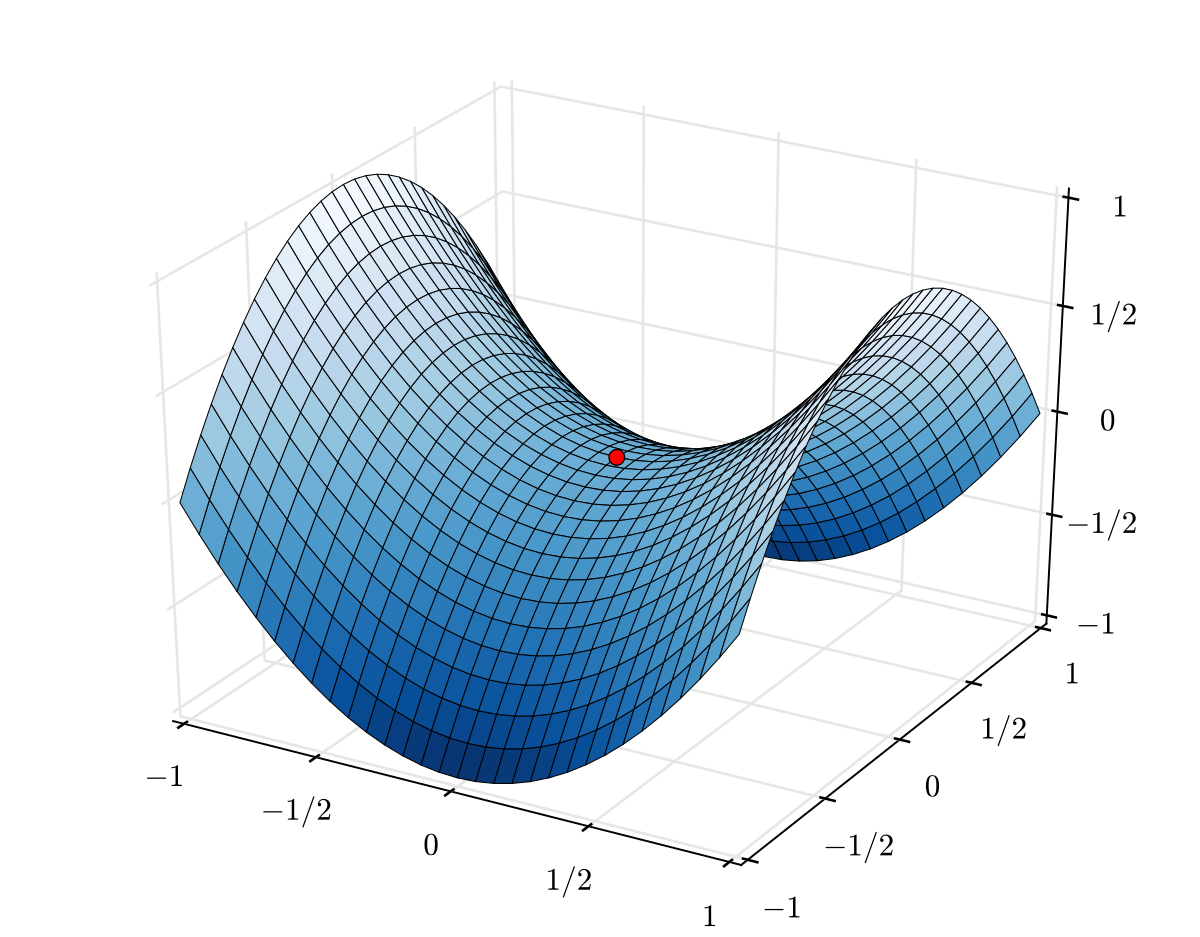
\includegraphics[width=0.8\columnwidth]{figures/saddle_point}
\end{figure}
\end{column}
\end{columns}
\let\thefootnote\relax\footnotetext{\tiny{Reference: Chris De Sa's slides (CS6787 Lecture 7).}}
\end{frame}

\begin{frame}{Learning rate}
\begin{itemize}
\item One of the most important hyperparameter.
\item Start with a higher learning rate then decay towards zero.
\pause
\item Classic theory: convergence guarantee for stochastic gradient descent. Otherwise the update step has a noise term dominated by the noise of data sample.
\item Other explanation: Loss surface, avoidance of local minima, avoidance of memorization of noisy samples
\pause
\item Learning rate decay (staircase 10x, cosine, etc.), speeds up convergence
\end{itemize}
\end{frame}

% \begin{frame}{More in-depth topics}
% \begin{itemize}
%     \item<+-> Neural networks have been a popular machine learning model in the past decade, due to its learning capability.
%     \item<+-> Today: MLP + SGD (backprop)
%     \item<+-> Adding structures: weight-sharing, convolution, recurrent, residual connection, attention
%     \item<+-> Learning conditioning: normalization, optimizers
%     \item<+-> Learning tasks: generative modeling, 3D perception, planning \& control
%     \item<+-> System: GPU/TPU, parallel computing, gradient aggregation
%     \item<+-> Some topics covered in DS-GA 1008 Deep Learning
% \end{itemize}
% \end{frame}

\begin{frame}{Biological Plausibility}
\begin{itemize}
    \item<+-> Backprop is used to train the overwhelming majority of neural nets today.
    \item<+-> Despite its practical success, backprop is believed to be neurally implausible.
    \item<+-> No evidence for biological signals analogous to error derivatives.
    \item<+-> Two main problems with implementing in an asynchronous analog hardware like our brain.
    % \item<+-> Forward \& backward weights are tied in backprop.
    % \item<+-> Backprop requires synchronous update (1 forward followed by 1 backward).
    % \item<+-> Biologically plausible alternatives we know about learn much more slowly on computers.
\end{itemize}
\end{frame}

\begin{frame}{Biological Plausibility}
\begin{center}
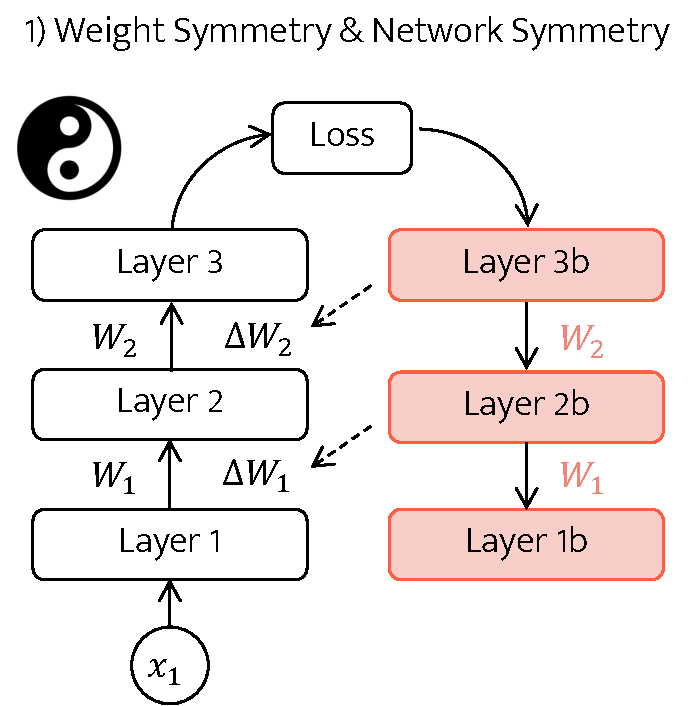
\includegraphics[height=0.7\textheight]{figures/symmetry.pdf}
\quad
\pause
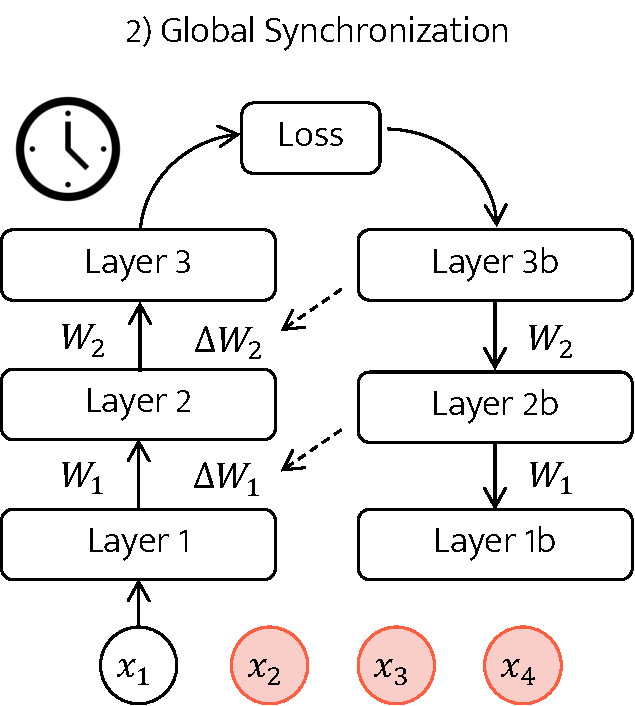
\includegraphics[height=0.7\textheight]{figures/synchronization.pdf}
\end{center}
\end{frame}

\begin{frame}
{Review}
\begin{itemize}
\item<+-> Backpropagation is an algorithm for computing the gradient (partial derivatives + chain rule) efficiently.
\item<+-> It is used in gradient descent optimization for neural networks.
\item<+-> Key idea: function composition and the chain rule
% \item Key idea: function composition and dynamic programming
\item<+-> In practice, we can use existing software packages, e.g. PyTorch (backpropagation, neural network building blocks, optimization algorithms etc.)
\end{itemize}
\end{frame}

\section{Weight sharing}
\begin{frame}{Applying Neural Networks on Images}
\begin{itemize}
    \item Neural networks are widely used on images today.
    \item Images are challenging to deal with because of its large dimensions.
    \pause
    \item Stored the intensity value pixel by pixel.
    \item A $28 \times 28$ image of digit 4:
\end{itemize}
\begin{center}
    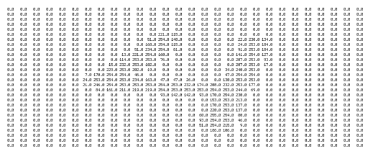
\includegraphics{figures/digit4.png}
\end{center}
% 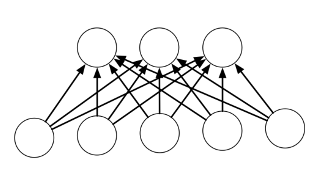
\includegraphics{figures/fully_connected.png}
% 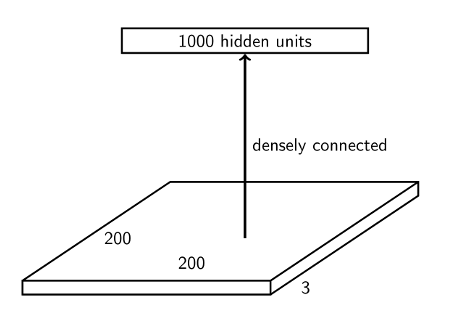
\includegraphics{figures/nn_1000_hidden.png}
\end{frame}

\begin{frame}{Fully connected vs. locally connected}
\begin{itemize}
    \item So far we apply a layer where all output neurons are connected to all input neurons.
    \item In matrix form, $\mathbf{z} = W \mathbf{x}$.
    \item This is also called a fully connected layer or a dense layer or a linear layer.
    \pause
    \item For $200 \times 200$ image and 1000 hidden units, the matrix of a single layer will have 40M parameters!
\end{itemize}
\begin{center}
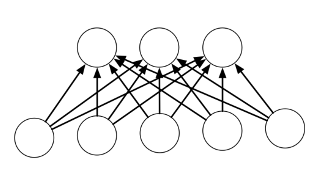
\includegraphics[width=0.34\textwidth]{figures/fully_connected.png}
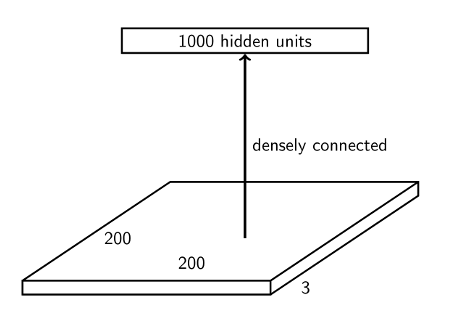
\includegraphics[width=0.34\textwidth]{figures/nn_1000_hidden.png}
\end{center}
\end{frame}
\begin{frame}{Fully connected vs. locally connected}
\begin{itemize}
    \item An alternative strategy is to use local connection.
    \item For neuron i, only connects to its neighborhood (e.g. [i+k, i-k])
    \item For images, we index neurons with three dimensions i, j, and c.
    \item i = vertical index, j = horizontal index, c = channel index.
\end{itemize}
\begin{center}
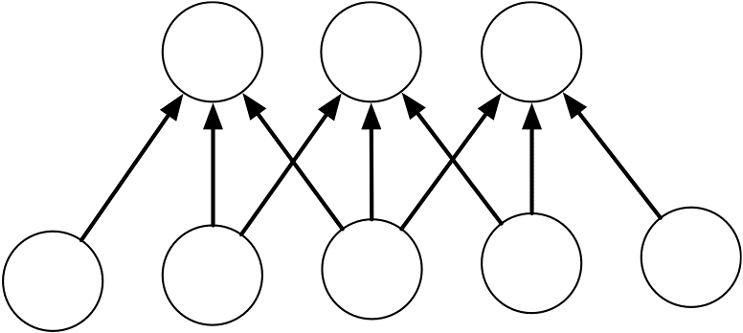
\includegraphics[width=0.3\textwidth]{figures/locally_connected.png}
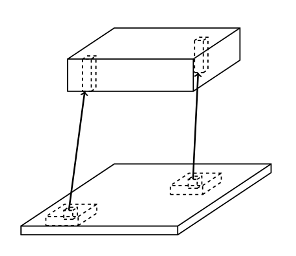
\includegraphics[width=0.3\textwidth]{figures/locally_connected_3d.png}
\end{center}
\end{frame}

\begin{frame}{Local connection patterns}
\begin{columns}
\begin{column}{0.65\textwidth}
\begin{itemize}
    \onslide<1->{\item The typical image input layer has 3 channels R G B for color or 1 channel for grayscale.
    \item The hidden layers may have $C$ channels, at each spatial location $(i, j)$.
    }
    \onslide<2->{
    \item Now each hidden neuron $z_{i,j,c}$ receives inputs from $x_{i \pm k, j \pm k, \cdot}$ 
    % - taking all the channels at neighboring spatial locations.
    \item $k$ is the ``kernel'' size - do not confuse with the other kernel we learned.
    \item $z_{i,j,c} = \sum_{i'\in[i\pm k], j' \in [j \pm k], c'} x_{i'j'c'} \textcolor{red}{w_{i, j, i'-i, j'-j, c',c}}$
    }
    \onslide<3->{
    \item The spatial awareness (receptive field) of the neighborhood grows bigger as we go deeper.
    }
\end{itemize}
\end{column}
\begin{column}{0.34\textwidth}
\begin{center}
\onslide<1->{
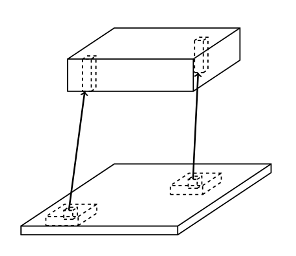
\includegraphics[width=0.8\textwidth]{figures/locally_connected_3d.png}
}
\end{center}
\end{column}
\end{columns}
\end{frame}

\begin{frame}{Weight sharing}
\begin{itemize}
\item Still a lot of weights: If we have 100 channels in the second layer, then $200 \times 200 \times 3 \times 100 = 12M$
\pause
\item Local information is the same regardless of the position of an element.
% \item E.g. A dog is a dog anywhere in an image.
\pause
\item Solution: We can tie the weights at different locations.
\end{itemize}
\begin{center}
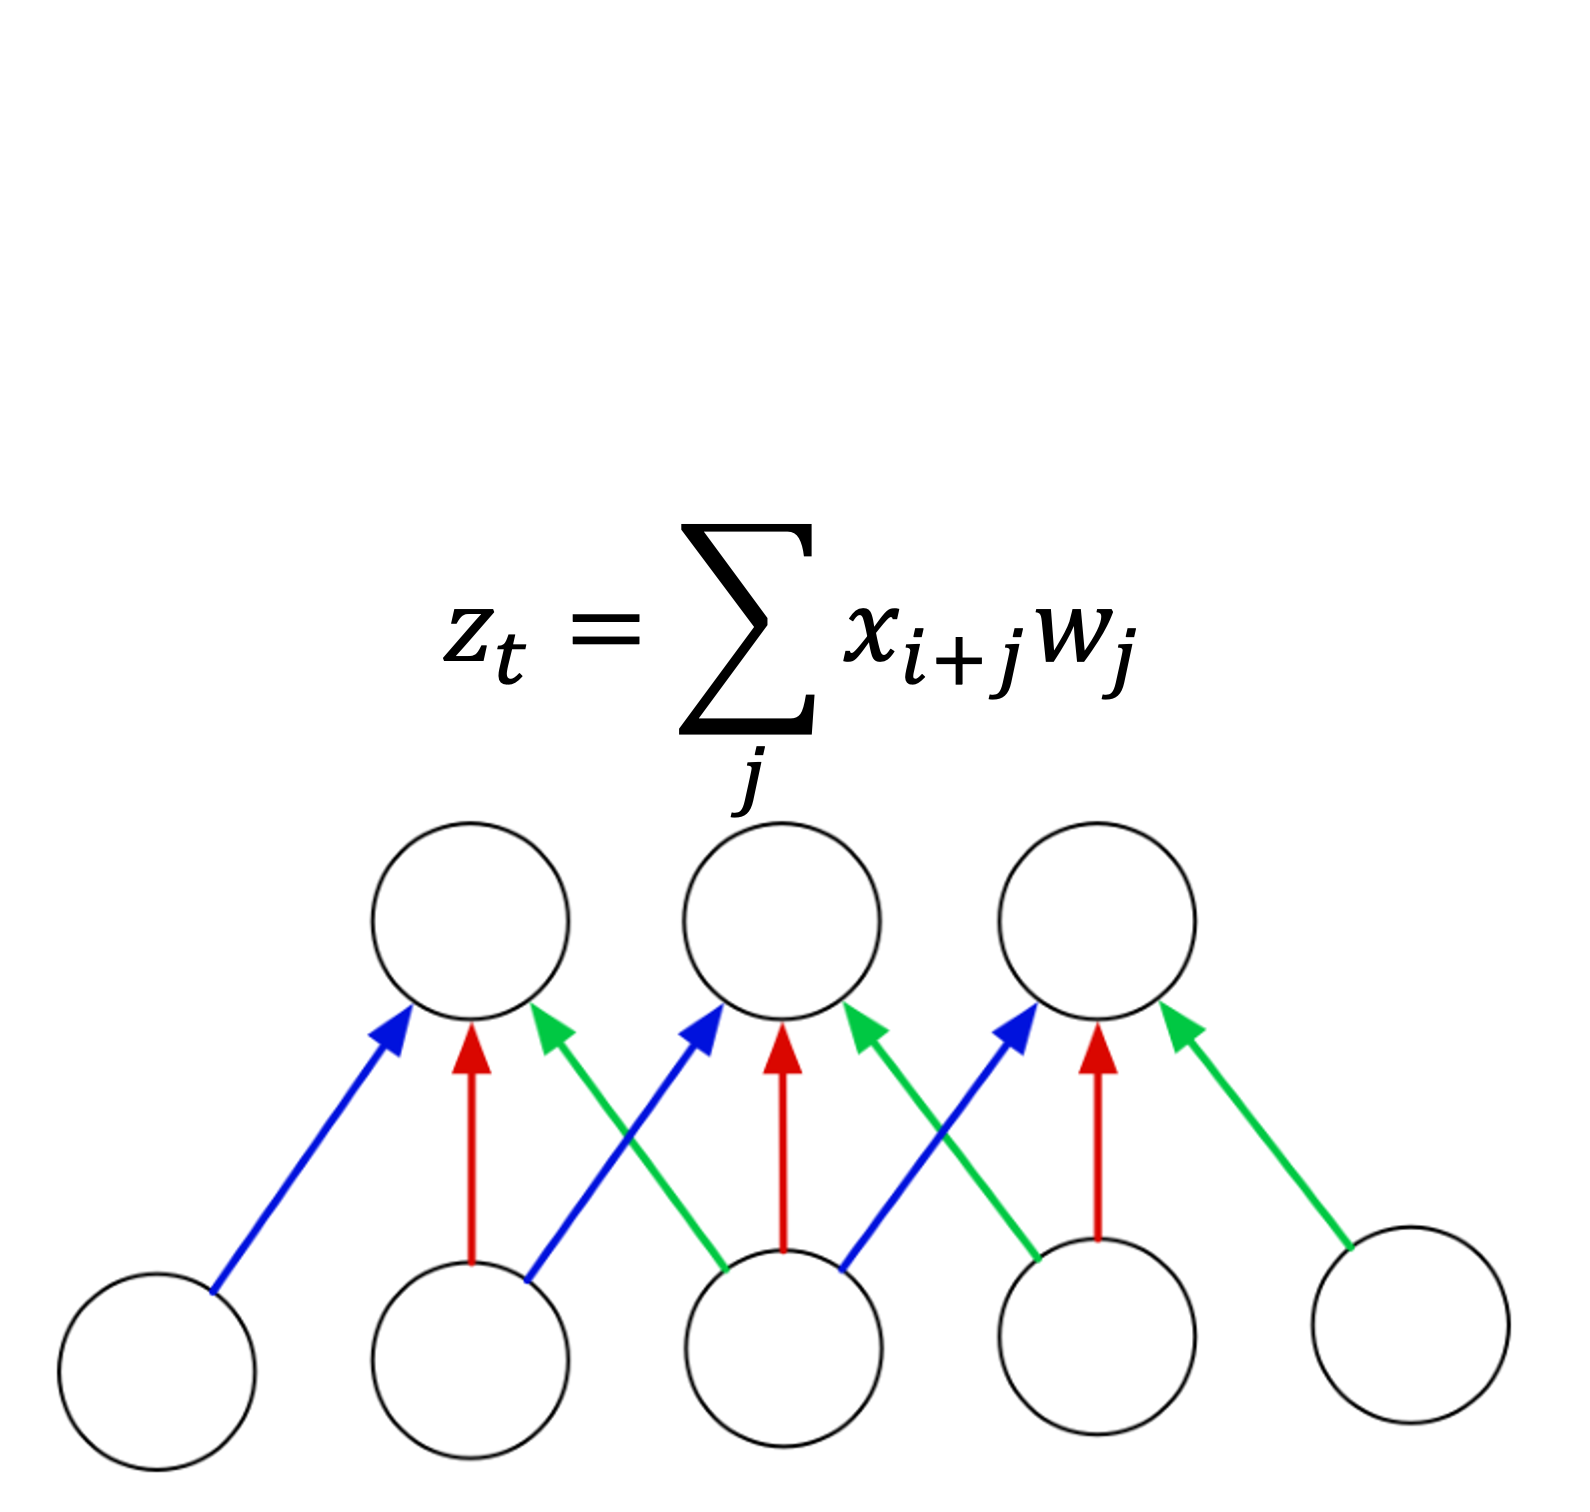
\includegraphics[width=0.3\textwidth,trim={0 0 0 6.2cm},clip]{figures/weight_share_2d.png}
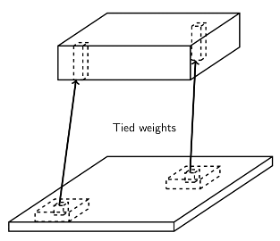
\includegraphics[width=0.3\textwidth]{figures/weight_share_3d.png}
\end{center}
\end{frame}

\begin{frame}{2D convolution}

\begin{columns}
\begin{column}{0.5\textwidth}
\begin{itemize}
    \item Using the same weight connections for each activation spatial location works like the ``filtering operation'' or ``convolution''
    \item The neighborhood window is the filter window.
    \item The weight connection is called ``convolution filter''
    \item $z_{i,j,c} = \sum_{i'\in[i\pm k], j' \in [j \pm k], c'} x_{i'j'c'} \textcolor{red}{w_{i-i', j-j', c',c}}$
\end{itemize}
\end{column}
\begin{column}{0.5\textwidth}
\begin{center}
\includegraphics<1>[width=0.8\textwidth]{figures/2d_conv/frame_0.png}
\includegraphics<2>[width=0.8\textwidth]{figures/2d_conv/frame_1.png}
\includegraphics<3>[width=0.8\textwidth]{figures/2d_conv/frame_2.png}
\includegraphics<4>[width=0.8\textwidth]{figures/2d_conv/frame_3.png}
\includegraphics<5>[width=0.8\textwidth]{figures/2d_conv/frame_4.png}
\includegraphics<6>[width=0.8\textwidth]{figures/2d_conv/frame_5.png}
\includegraphics<7>[width=0.8\textwidth]{figures/2d_conv/frame_6.png}
\includegraphics<8>[width=0.8\textwidth]{figures/2d_conv/frame_7.png}
\includegraphics<9>[width=0.8\textwidth]{figures/2d_conv/frame_8.png}
\end{center}
\end{column}
\end{columns}
\end{frame}


\begin{frame}{Pooling}
\begin{columns}
\begin{column}{0.5\textwidth}
\begin{itemize}
    \item Need to summarize global information more efficiently.
    \item Pooling reduces image / activation dimensions.
    \item Max-pooling or average-pooling
    \onslide<2->{
    \item You can also perform a ``strided'' convolution by jumping multiple steps.
    }
\end{itemize}
\end{column}
\begin{column}{0.5\textwidth}
\begin{center}
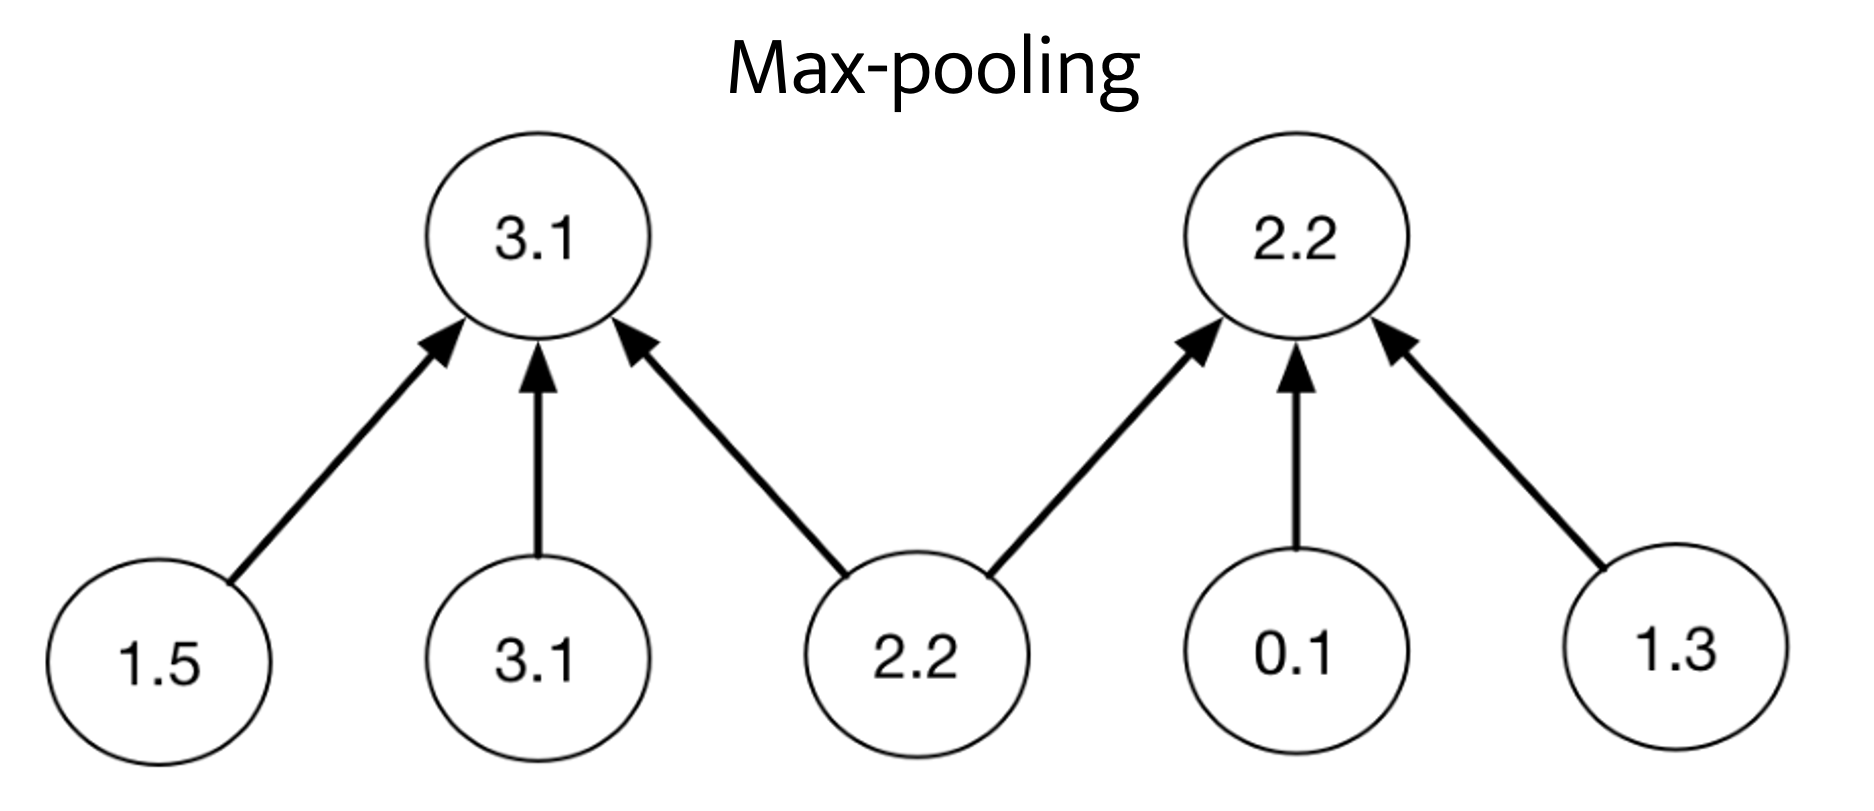
\includegraphics[width=0.8\textwidth]{figures/maxpooling.png}
\includegraphics<2>[width=0.5\textwidth]{figures/stride2_conv/frame_0.png}
\includegraphics<3>[width=0.5\textwidth]{figures/stride2_conv/frame_1.png}
\includegraphics<4>[width=0.5\textwidth]{figures/stride2_conv/frame_2.png}
\includegraphics<5>[width=0.5\textwidth]{figures/stride2_conv/frame_3.png}
\end{center}
\end{column}
\end{columns}
\end{frame}

\begin{frame}{Assembling together: LeNet}
\begin{center}
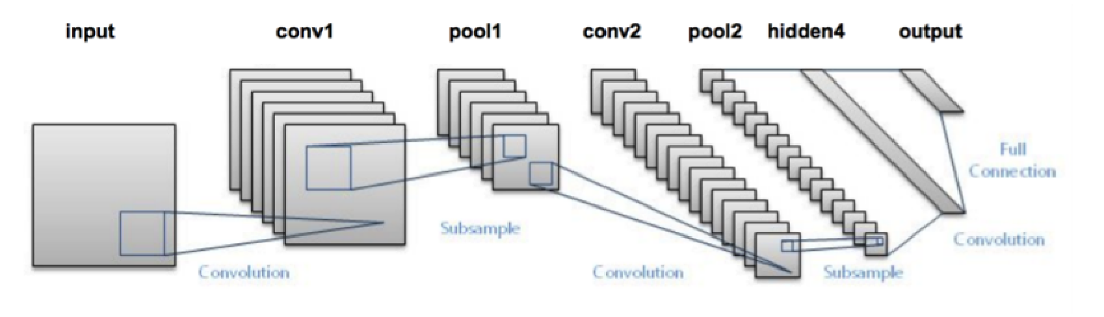
\includegraphics[width=0.8\textwidth]{figures/lenet2.png}
\end{center}
\begin{itemize}
    \item Used by USPS to read post code in the 90s.
\end{itemize}
\end{frame}

\begin{frame}{Historical development}
\begin{itemize}
    \item LeNet has worked and being put to practice in the 1990s.
    \pause
    \item Neural networks for images start to dominate in the last 10 years (starting 2012) for understanding general high resolution natural images.
    \pause
    \item During the years:
    \begin{itemize}
        \item Neural networks were difficult to work
        \item People focused on feature engineering
        \item Then apply SVM or random forest (e.g. AdaBoost face detector)
        \item What has changed?
    \end{itemize}
\end{itemize}
\end{frame}

\section{Gradient learning conditioning}
\begin{frame}{Optimization challenges}
\begin{itemize}
    \item Larger images require deeper networks (more stages of processing at different resolutions)
    \item Optimizing deeper layers of networks is not trivial.
    \item Loss often stalls or blows up.
    \item Why?
    \pause
    \begin{itemize}
        \item Backpropagation: multiplying the Jacobian $\frac{\partial y}{\partial x}$ by each layer.
        \item If the maximum singular value of each layer of Jacobian is less than 1: then the gradient will converge to 0 with more layers.
        \item If the greater than 1: then the gradient will explode with more layers.
        \item The bottom (input) layer may get 0 or infinite gradients.
    \end{itemize}
\end{itemize}
\end{frame}

\begin{frame}{Weight initialization}
\begin{itemize}
    \item Even with a few layers (>3), optimization is still hard.
    \item If weight initialization is bad (too small or too big), then optimization is hard to kick off.
    \item Consider the distribution of whole dataset in the activation space.
    % \item Pre-activation: $z=Wx$; Post-activation: $h=f(z)$
    \begin{itemize}
        % \item The mean of the pre-activations should be zero.
        \item Intuition: upon initialization, the variance of the activations should stay the same across every layer.
    \end{itemize}
\end{itemize}
\end{frame}

\begin{frame}{Kaiming Initialization}
\begin{itemize}
    \item Suppose each neuron and weight connection are sampling from a random distribution.
    \pause
    \item At $l$-th layer, $Var[z_l] = n_l Var[w_l x_l]$ ($n_l$ = num. input neurons to $l$-th layer)
    \pause
    \item If we suppose that ReLU is used as the activation, and $w_l$ is symmetric and zero-mean, $x_{l+1} = \frac{1}{2} Var[z_{l}]$.
    \pause
    \item Putting altogether, $x_{l+1} = \frac{1}{2} n_l Var[w_{l}] Var[x_l]$.
    \pause
    \item To make the variance constant, we need $\frac{1}{2} n_l Var[w_{l}] = 1$, $Std[w_{l}] = \sqrt{2/n_l}$\footnote{He et al. Delving Deep into Rectifiers: Surpassing Human-Level Performance on ImageNet. ICCV, 2015.}.
\end{itemize}
\end{frame}

\begin{frame}{Activation functions}
\begin{itemize}
    \item ReLU was proposed in 2009-2010\footnote{Jarrett et al. What is the Best Multi-Stage Architecture for Object Recognition? ICCV, 2009.}\footnote{Nair \& Hinton/ Rectified Linear Units Improve Restricted Boltzmann Machines. ICML, 2010.}, and was successfully used in AlexNet in 2012\footnote{Krizhevsky et al. 
ImageNet Classification with Deep Convolutional Neural Networks. NIPS, 2012.}.
    \item Address the vanishing gradient issue in activations, comparing to sigmoid or tanh.
    % \item More variants of activation function in the past decade.
\end{itemize}
\begin{center}
    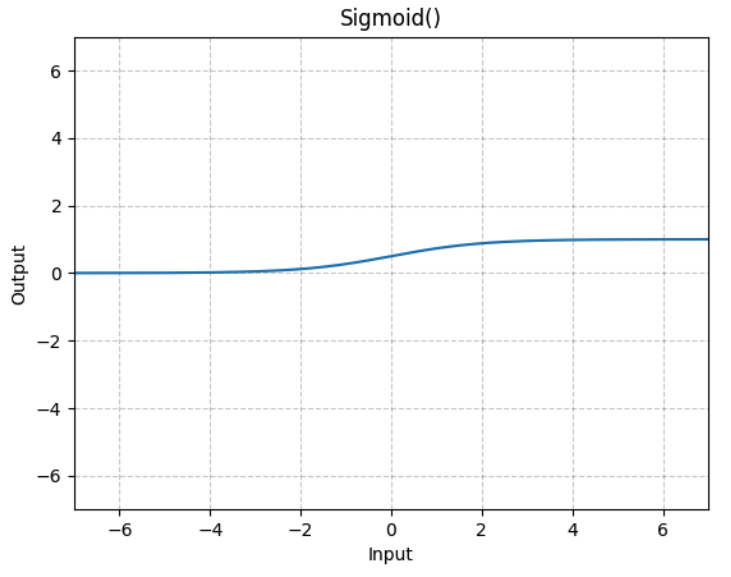
\includegraphics[width=0.17\textwidth]{figures/sigmoid.png}
    \quad
    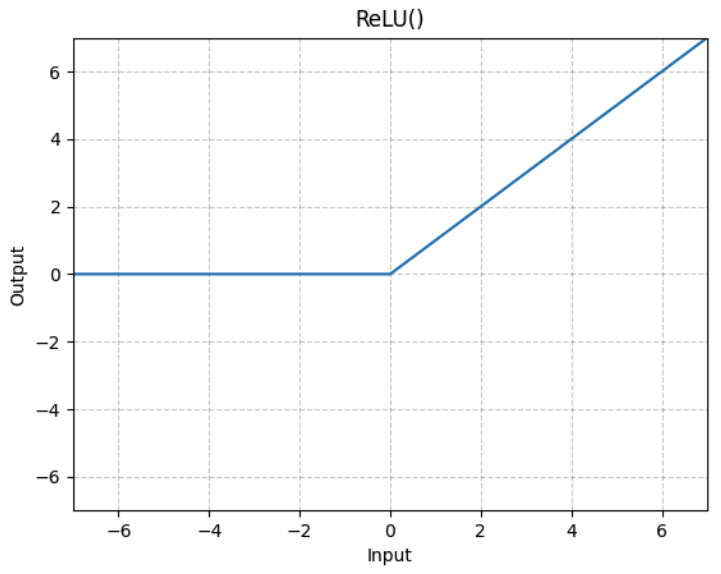
\includegraphics[width=0.17\textwidth]{figures/relu.png}
    \quad
    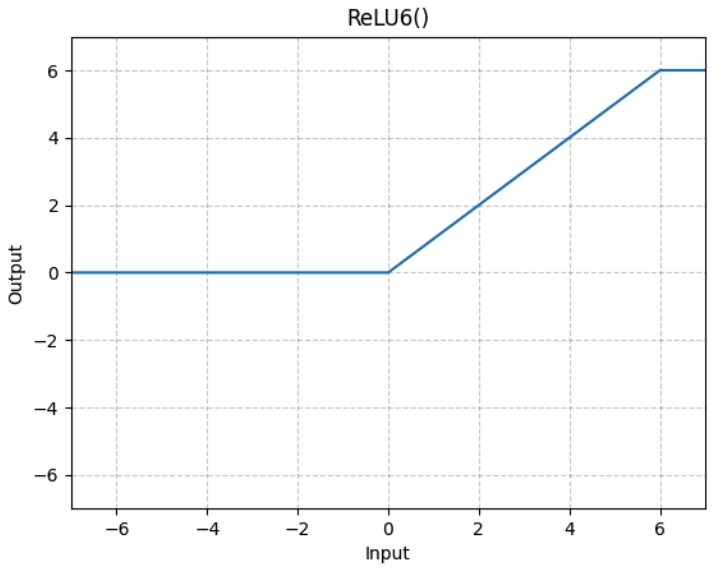
\includegraphics[width=0.17\textwidth]{figures/relu6.png}

    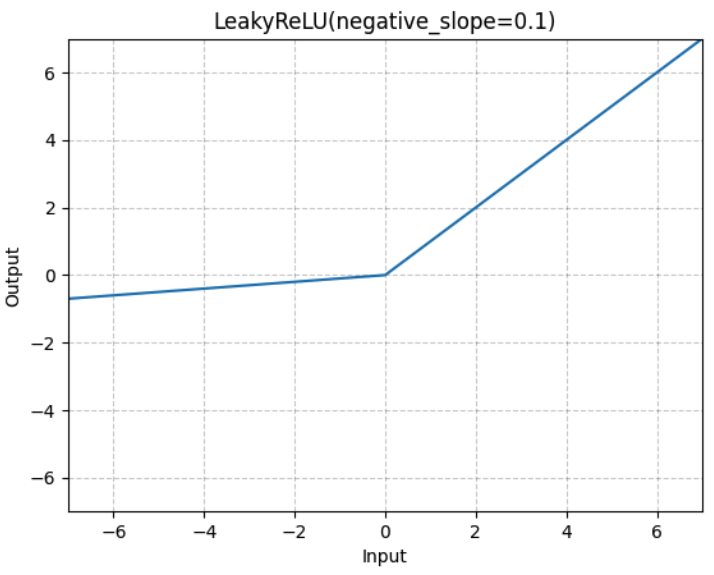
\includegraphics[width=0.17\textwidth]{figures/leaky_relu.png}
    \quad
    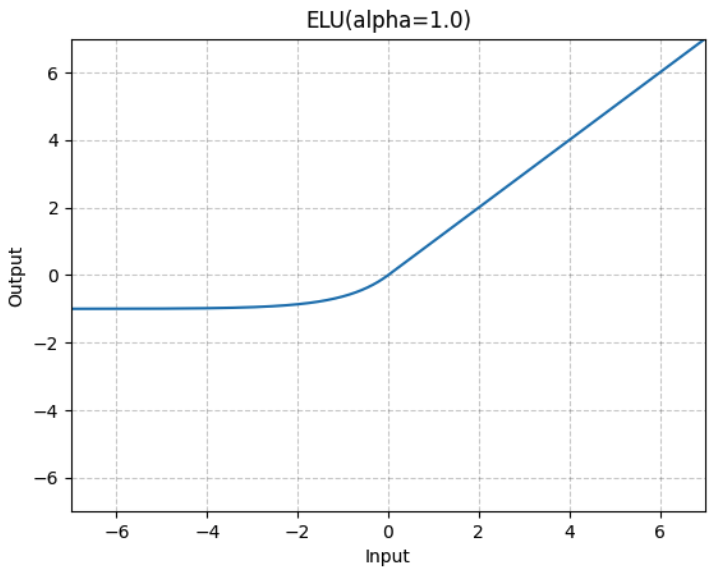
\includegraphics[width=0.17\textwidth]{figures/elu.png}
    \quad
    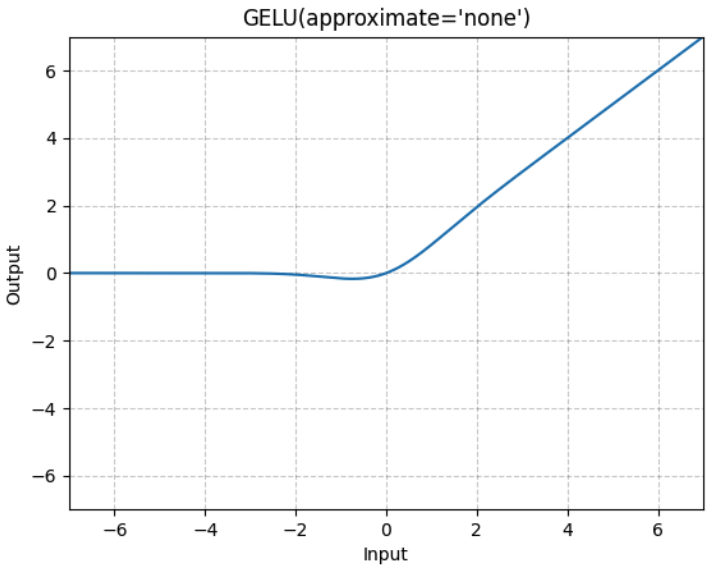
\includegraphics[width=0.17\textwidth]{figures/gelu.png}
\end{center}
\end{frame}

\begin{frame}{SGD Learning Rate}
  \begin{itemize}
    \item In stochastic training, the learning rate also influences the \alert{fluctuations} due to the stochasticity of the gradients.
    \item Typical strategy:
      \begin{itemize}
        \item Use a large learning rate early in training so you can get close to the optimum
        \item Gradually decay the learning rate to reduce the fluctuations
      \end{itemize}
  \end{itemize}
\end{frame}

\begin{frame}{Learning Rate Decay}
    \begin{itemize}
      \item We also need to be aware about the impact of learning rate due to the stochasticity.
    \end{itemize}
    \begin{center}
      \includegraphics[width=0.3\textwidth]{figures/fluctuations.png}
    \end{center}
    \begin{center}
      \includegraphics[width=0.25\linewidth]{figures/premature_lr_decay.png}
      \hspace{0.05 \linewidth}
      \includegraphics[width=0.25\linewidth]{figures/sgd_learning_curves.png}
    \end{center}
\end{frame}

\begin{frame}{RMSprop and Adam}
  \begin{itemize}
  \item Recall: SGD takes large steps in directions of high curvature and small steps in directions of low curvature.
  \item \alert{RMSprop} is a variant of SGD which rescales each coordinate of the gradient to have norm 1 on average. It does this by keeping an exponential moving average $s_j$ of the squared gradients.
  \item The following update is applied to each coordinate $j$ independently:
    \begin{align*}
      s_j &\gets (1-\gamma) s_j + \gamma [\tfrac{\partial L}{\partial \theta_j}]^2 \\
      \theta_j &\gets \theta_j - \frac{\alpha}{\sqrt{s_j + \epsilon}} \frac{\partial L}{\partial \theta_j}
    \end{align*}
  % \item Both optimizers are included in TensorFlow, Pytorch, etc.
  \end{itemize}
  % \notenew{
  % \begin{itemize}
  %   \item Draw a skewed axis-aligned quadratic.
  %   \item If the eigenvectors of the Hessian are axis-aligned (dubious assumption), then RMSprop can correct for the curvature. In practice, it typically works slightly better than SGD.
  % \end{itemize}
  % }
\end{frame}

\begin{frame}{Adam optimizer}
\begin{columns}
\begin{column}{0.6\textwidth}
\begin{itemize}
  \item \alert{Adam} = RMSprop + momentum = Adaptive Momentum estimation
  \item Smoother estimate of the average gradient and gradient norm.
  \item $m_t$: exponential moving average of gradient.
  \item $v_t$: exponential moving average of gradient squared.
  \item $\hat{m}_t$, $\hat{v}_t$: Bias correction.
  \item $\theta_t \leftarrow \theta_{t-1} - \alpha \hat{m}_t / (\sqrt{\hat{v_t}} + \epsilon)$
  \item The ``default'' optimizer for modern networks.
\end{itemize}
\end{column}
\begin{column}{0.38\textwidth}
\begin{center}
\includegraphics[width=0.8\textwidth]{figures/adam.png}
\end{center}
\end{column}
\end{columns}
\end{frame}

\begin{frame}{Normalization}
% \begin{columns}
% \begin{column}{0.6\textwidth}
\begin{itemize}
    \item Weight initialization is tricky, and there is no guarantee that the distribution of activations will stay the same over the learning process.
    \item What if the weights keep grow bigger and activation may explode?
    \item We can ``normalize'' the activations.
    \item The idea is to control the activation within a normal range: zero-mean, uni-variance.
\end{itemize}
% \end{column}
% \begin{column}{0.38\textwidth}
% \begin{center}
% \includegraphics[width=0.8\textwidth]{figures/normalization.png}
% \end{center}
% \end{column}
% \end{columns}
\end{frame}

\begin{frame}{Batch Normalization (BN)}

\begin{columns}
\begin{column}{0.6\textwidth}
\begin{itemize}
    % \item What is the population to normalize it from?
    \item Training image distribution -> activation distribution
    \item In CNNs, neurons across different spatial locations are also samples of the same feature channel.
    \item Batch norm: Normalize across N H W dimensions, leaving C channels.
    \item $\tilde{x} = \gamma \frac{x - \mu}{\sigma} + \beta$
    \item Test time: using the mean and variance from the entire training set.
\end{itemize}
\end{column}

\begin{column}{0.38\textwidth}
\begin{center}
\includegraphics[width=0.7\textwidth,trim={0 0 25.5cm 0},clip]{figures/normalization.png}
\end{center}
\end{column}
\end{columns}

\end{frame}

\begin{frame}{BN Alternatives}
\begin{itemize}
    \item Need a considerable batch size to estimate mean and variance correctly.
    \item Training is different from testing.
    \item Alternatives consider the C channel dimension instead of N batch dimension.
    % \item No longer estimating the distribution from training samples.
\end{itemize}
\begin{center}
\includegraphics[width=0.7\textwidth,trim={10cm 0 0 0},clip]{figures/normalization.png}
\end{center}
\end{frame}

\begin{frame}{Going Deeper}
\begin{itemize}
    \item The progress of normalization allowed us to train even deeper networks.
    \item The networks are no longer too sensitive with initialization.
    \item But the best networks were still around 20 layers and deeper results in worse performance.
\end{itemize}
\begin{center}
\includegraphics[width=0.6\textwidth]{figures/googlenet.png}
\includegraphics[width=0.35\textwidth]{figures/20layer.png}
\end{center}
\end{frame}

% \begin{frame}{Residual Networks}
% \begin{itemize}
%     \item Recall in gradient boosting, we are iteratively adding a function to the model to expand the capacity.
%     \item 
% \end{itemize}
% \end{frame}

\begin{frame}{Residual Networks (ResNet)}

\begin{itemize}
    \item Recall in gradient boosting, we are iteratively adding a function to the model to expand the capacity.
    \item Residual connection: Skip connection to prevent gradient vanishing.\footnote{He et al. Deep Residual Learning for Image Recognition. CVPR 2016.}
    % \item A simple ``addition'' operation on the activation.
\end{itemize}

\begin{center}
% \includegraphics[width=0.75\textwidth]{figures/residual_connect.png}
\includegraphics[width=0.5\textwidth]{figures/resnet.png}
\end{center}

\end{frame}

\begin{frame}{ResNet Success}
\begin{itemize}
    \item Now able to train over 100 layers.
    \item One of the most important network design choices in the past decade.
    \item Prevalent in almost all network architectures, including Transformers.
    \item Loss landscape view: Skip connections makes loss smoother -> easier to optimize \footnote{Li et al. Visualizing the Loss Landscape of Neural Nets. NIPS 2018.}.
\end{itemize}
\begin{center}
% \includegraphics[width=0.75\textwidth]{figures/residual_connect.png}
\includegraphics[width=0.5\textwidth]{figures/resnetlandscape.png}
\end{center}
\end{frame}

\begin{frame}{Dropout\footnote{Srivastava et al. A Simple Way to Prevent Neural Networks from Overfitting. JMLR, 2014.}
}
\begin{itemize}
    \item Want to reduce overfitting in neural networks.
    \item Stochastically turning off neurons in propagation.
    \onslide<2->{
    \item Training to preserve redundancy.
    \item Test time: multiplying activations with probability. Model ensembling effect.
    }
\end{itemize}
\begin{center}
\onslide<1->{
\includegraphics[width=0.4\textwidth]{figures/dropout.png}
}
\end{center}

\end{frame}

\begin{frame}{GELU\footnote{Hendrycks \& Gimpel. Gaussian Error Linear Unit (GELU). CoRR abs/1606.08415, 2016.}}
\begin{columns}
\begin{column}{0.49\textwidth}
\begin{itemize}
    \item Gaussian Error Linear Unit - A smoother activation function. 
    \item Motivated by Dropout.
    \onslide<2->{
    \item $f(x) = \mathbb{E}[x \cdot m].$
    }
    \onslide<3->{
    \item $m \sim Bernoulli(\Phi(x)).$
    \item $\Phi(x) = P(X \le x).$
    \item $X \sim \mathcal{N}(0,1).$
    }
\end{itemize}
\end{column}
\begin{column}{0.49\textwidth}
\begin{center}
    \onslide<1->{\includegraphics[width=0.8\textwidth]{figures/gelu.png}}
\end{center}
\end{column}
\end{columns}
\end{frame}

\begin{frame}{Data augmentation}
\begin{columns}
\begin{column}{0.4\textwidth}
\begin{itemize}
    \item Leverage the invariances of images
    \item Create more data points for free
    \begin{itemize}
    \item<2->Random cropping
    \item<3->Left+right flipping
    \item<4->Random color jittering
    \item<5->Random blurring
    \item<6->Affine warping
    \item<6->Etc.
    \end{itemize}
\end{itemize}
\end{column}
\begin{column}{0.59\textwidth}
\onslide<1->\includegraphics[width=0.9\textwidth]{figures/data_aug.png}
\end{column}
\end{columns}
    \small{Image credit}\footnote{Chen et al. A Simple Framework for Contrastive Learning of Visual Representations. ICML 2020.}
\end{frame}


\section{Language and sequential signals}
\begin{frame}{What about natural language}
\begin{itemize}
    \item<+-> Neural networks are great for dealing with naturalistic and unstructured signals.
     % such as images, sound, language, where there are no good manual feature extractors.
    \item<+-> Past lectures: Feature functions in structured models, but still primitive.
    \item<+-> Design neural networks to accomodate sequential signals such as language.
\end{itemize}
\begin{center}
\onslide<1->\includegraphics[width=0.7\textwidth,trim={0 0 0 3cm},clip]{figures/neural-machine-translation.png}
\end{center}
\end{frame}

\begin{frame}{Word embeddings}
\begin{itemize}
    \item<+-> Neural networks are best dealing with real valued vectors.
    \item<+-> Need to convert words (discrete) into vectors (continuous).
    \item<+-> A large matrix of $V \times D$. V = vocab size, D = network embedding size.
\end{itemize}
\begin{center}
\includegraphics[width=0.4\textwidth]{figures/word_embedding.png}\footnote{https://aelang.github.io/word-embeddings.html}
\end{center}
\end{frame}

% \begin{frame}{Convolutional vs. recurrent networks}
% \begin{itemize}
%     \item Recall in images we used the convolution operation.
%     \item We can also use the idea of convolution for temporal signals.
% \end{itemize}
% \end{frame}

% \begin{frame}{Gating functions}
% \end{frame}

% \begin{frame}{Attention}
% \end{frame}

% \begin{frame}{Transformers}
% \end{frame}

% \begin{frame}{Autoregressive modeling}
% \end{frame}

% \begin{frame}{Multi-modal learning}
% \end{frame}

% \begin{frame}{Visual attention}
% \end{frame}

% \begin{frame}{Visual question answering}
% \end{frame}

% \begin{frame}{Interim Summary}
% \end{frame}

% \section{Interpretability}

% \begin{frame}{ML Interpretability}
% \begin{itemize}
%   \item Linear regression: Weights represent feature selection strength
%   \item SVMs: Dual weights represent sample selection
%   \item Bayesian methods: Model the generative process as a probabilistic model, fully transparent
%   \item Decision trees: If-else decision making process
%   \item Neural networks: ?
% \end{itemize}
% \end{frame}

% \begin{frame}{Feature Visualization}
% \begin{itemize}
%   \item Recall: we can understand what first-layer features are doing by visualizing the weight matrices.
%   \item Higher-level weight matrices are hard to interpret.
%   \begin{center}
%     \begin{columns}
%       \begin{column}{0.35 \textwidth}
%         \begin{center}
%           Fully connected
%           \includegraphics[width=0.6 \textwidth]{figures/mnist_filters.png}
%         \end{center}
%       \end{column}
%       \begin{column}{0.35 \textwidth}
%         \begin{center}
%           Convolutional
%           \includegraphics[width=0.55 \textwidth]{figures/zeiler_filters.pdf}
%         \end{center}
%         \begin{flushright}
%   \tiny{Zeiler and Fergus, Visualizing and understanding convolutional networks, ECCV 2014.}
%         \end{flushright}
%       \end{column}
%     \end{columns}
%   \end{center}
% \item The better the input matches these weights, the more the feature activates.
%   \begin{itemize}
%   \item Obvious generalization: visualize higher-level features by seeing what inputs activate them.
%   \end{itemize}
% \end{itemize}
% \end{frame}

% \begin{frame}{Feature Visualization}
% \begin{itemize}
% \item One way to formalize: pick the images in the training set which activate a unit most strongly.
% \item Here's the visualization for layer 1:
%   \begin{center}
%     \includegraphics[width=0.3 \textwidth]{figures/layer1.png}
%   \end{center}
% \end{itemize}
% \begin{flushright}
%   \tiny{Zeiler and Fergus, Visualizing and understanding convolutional networks, ECCV 2014.}
% \end{flushright}
% \end{frame}

% \begin{frame}{Feature Visualization}
% \begin{itemize}
% \item Layer 3:
%   \begin{center}
%     \includegraphics[width=0.4 \textwidth]{figures/layer3.png}
%   \end{center}
% \end{itemize}
% \begin{flushright}
%   \tiny{Zeiler and Fergus, Visualizing and understanding convolutional networks, ECCV 2014.}
% \end{flushright}
% \end{frame}

% \begin{frame}{Feature Visualization}
% \begin{itemize}
% \item Layer 4:
%   \begin{center}
%     \includegraphics[width=0.4 \textwidth]{figures/layer4.png}
%   \end{center}
% \end{itemize}
% \begin{flushright}
%   \tiny{Zeiler and Fergus, Visualizing and understanding convolutional networks, ECCV 2014.}
% \end{flushright}
% \end{frame}

% \begin{frame}{Feature Visualization}
% \begin{itemize}
% \item Layer 5:
%   \begin{center}
%     \includegraphics[width=0.7 \textwidth]{figures/layer5.png}
%   \end{center}
% \end{itemize}
% \begin{flushright}
%   \tiny{Zeiler and Fergus, Visualizing and understanding convolutional networks, ECCV 2014.}
% \end{flushright}
% \end{frame}

% \begin{frame}{Feature Visualization}
% \begin{itemize}
%   \item Higher layers seem to pick up more abstract, high-level information.
%   \item Problems?
%     \begin{itemize}
%     \item Can't tell what the unit is actually responding to in the image.
%     \item We may read too much into the results, e.g.~a unit may detect red, and the images that maximize its activation will all be stop signs.
%     \end{itemize}
%   \item Can use input gradients to diagnose what the unit is responding to.
% \end{itemize}
% \end{frame}

% \begin{frame}{Feature Visualization}
% \begin{itemize}
% \item Input gradients can be hard to interpret.
% \item Take a good object recognition conv net (Alex Net) and compute the gradient of $\log p(y= \textrm{``cat''} | \mathbf{x})$:
%   \begin{center}
%     \begin{columns}
%       \begin{column}{0.35 \textwidth}
%         \begin{center}
%           Original image
%           \includegraphics[width=0.8 \textwidth]{figures/cat.pdf}
%         \end{center}
%       \end{column}
%       \begin{column}{0.35 \textwidth}
%         \begin{center}
%           Gradient for ``cat''
%           \includegraphics[width=0.7 \textwidth]{figures/cat_gradient.pdf}
%         \end{center}
%       \end{column}
%     \end{columns}
%   \end{center}
% \end{itemize}
% \end{frame}

% \begin{frame}{Feature Visualization}
%   \begin{itemize}
%   \item \alert{Guided backprop} is a total hack to prevent this cancellation.
%   \item Do the backward pass as normal, but apply the ReLU nonlinearity to all the activation error signals.
%     \[ y = \textrm{ReLU}(z) \qquad \bar{z} = \begin{cases} \bar{y} & \text{if $z > 0$ {\color{red} and $\bar{y} > 0$}} \\ 0 & \text{otherwise} \end{cases} \]
%   \item We want to visualize what excites given unit, not what suppresses it.
%     \begin{center}
%       \includegraphics[width=0.5 \textwidth]{figures/guided_backprop_results.pdf}
%     \end{center}
%   \end{itemize}
% \end{frame}

% \begin{frame}{Guided Backprop}
% \begin{center}
%   \includegraphics[width=0.85 \textwidth]{figures/guided_backprop_results2.pdf}
% \end{center}
% \begin{flushright}
% {\tiny Springerberg et al., Striving for simplicity: The all convolutional net, ICLR workshop 2015.}
% \end{flushright}

% % \notenew{
% % \begin{itemize}
% %   \item We start from here.
% %   \item Visualize one neuron in the input image.
% %   \item Draw one neuron in the middle.
% % \end{itemize}
% % }
% \end{frame}


% \begin{frame}{Class activation map (CAM)}

% Classification networks typically use global avg pooling before the final layer.

% This pooling layer can already contain semantic information.

% We can visualize a heat map 

% \begin{center}
% \includegraphics[height=0.3\textheight]{figures/cam.png}
% \includegraphics[height=0.3\textheight]{figures/cam2.png}
% \end{center}

% \begin{flushright}
% {\tiny Zhou et al. Learning deep features for discriminative localization. CVPR 2016.}
% \end{flushright}

% % \notenew{
% %   \begin{itemize}
% %     \item Another way is to think about the output classes.
% %     \item Imagine you have a classifier.
% %     \item What would be the region of the input that is responsible 
% %     \item Utilize the average pooling layer.
% %     \item Take the dot product between the activation at each location and the class vector
% %   \end{itemize}
% % }
% \end{frame}

% \begin{frame}{GradCAM}

% \begin{center}
% \vspace{-0.2in}
% \includegraphics[width=0.7\textwidth]{figures/gradcam.png}
% \includegraphics[width=0.45\textwidth,trim={0 0 16cm 0},clip]{figures/gradcam2.png}
% \end{center}

% \begin{flushright}
% {\tiny Selvaraju et al. Grad-CAM: Visual explanations from deep networks via gradient-based localization. ICCV 2017.}
% \end{flushright}

% % \notenew{
% %   \begin{itemize}
% %     \item Potentially a way to combine guided backprop and CAM.
% %     \item In the example, GBP is still plotting the dog, even though we are visualizing the cat neuron.
% %     \item We can suppress it by overlapping it with CAM.
% %   \end{itemize}
% % }
% \end{frame}

% \begin{frame}{Gradient Ascent on Images}
% \begin{itemize}
% \item Can do gradient ascent on an image to maximize the activation of a given neuron.
%   \begin{center}
%     \hspace{-3em}\includegraphics[width=\textwidth]{figures/distill_gd.png}
%   \end{center}
% \end{itemize}
% \begin{flushright}
%   \begin{tiny}
%     \vspace{-1em}
%     \url{https://distill.pub/2017/feature-visualization/}
%   \end{tiny}
% \end{flushright}

% % \notenew{
% %   \begin{itemize}
% %     \item Guided backpropagation = 1 step
% %     \item What if we run multiple steps of gradients?
% %   \end{itemize}
% % }
% \end{frame}

% \begin{frame}{Gradient Ascent on Images}
% \begin{center}
%   \hspace{-1em}\includegraphics[width=\textwidth]{figures/distill_why_optimize.png}
% \end{center}
% \begin{flushright}
%   \begin{tiny}
%     \vspace{-1em}
%     \url{https://distill.pub/2017/feature-visualization/}
%   \end{tiny}
% \end{flushright}

% % \notenew{
% %   \begin{itemize}
% %     \item For the same layer, we can run it on different units, and get different results.
% %     \item Above: dataset examples that maximizes neuron activation
% %     \item Below: optimized images that maximizes neuron activation
% %   \end{itemize}
% % }
% \end{frame}

% \begin{frame}{Gradient Ascent on Images}
% \begin{itemize}
%   \item Higher layers in the network often learn higher-level, more interpretable representations
%     \begin{center}
%       \includegraphics[width=0.85 \linewidth]{figures/olah.png}
%     \end{center}
%     \begin{flushright}
%       \begin{tiny}
%         \vspace{-1em}
%         \url{https://distill.pub/2017/feature-visualization/}
%       \end{tiny}
%     \end{flushright}
% \end{itemize}
% \end{frame}

% \begin{frame}{Gradient Ascent on Images}
% \begin{itemize}
%   \item Higher layers in the network often learn higher-level, more interpretable representations
%     \begin{center}
%       \includegraphics[width=0.6 \linewidth]{figures/olah2.png}
%     \end{center}
%     \begin{flushright}
%       \begin{tiny}
%         \vspace{-1em}
%         \url{https://distill.pub/2017/feature-visualization/}
%       \end{tiny}
%     \end{flushright}
% \end{itemize}
% \end{frame}

% \begin{frame}{Deep dream}
% \begin{itemize}
% \item Start with an image, and run a conv net on it.
% \item Change the image such that units which were already highly activated get activated even more strongly.
% ``Rich get richer.''
% \end{itemize}
% \begin{center}
%   \hspace{-1em}\includegraphics[width=\textwidth]{figures/deepdream1.pdf}
% \end{center}

% % \notenew{
% % \begin{itemize}
% %   \item What if we try to maximize all neuron in one layer at once?
% % \end{itemize}
% % }
% \end{frame}

% \begin{frame}{Deep dream}
% \begin{center}
%   \hspace{-1em}\includegraphics[width=\textwidth]{figures/deepdream2.pdf}
% \end{center}
% \end{frame}

% \begin{frame}{Deep dream}
% \begin{center}
%   \hspace{-1em}\includegraphics[width=0.9\textwidth]{figures/deepdream3.pdf}
% \end{center}
% \end{frame}

% \begin{frame}{Artistic style transfer}
% \begin{itemize}
% \item Activation stores content information
% \item Activation correlation across space stores style information and discards spatial arrangement
% \end{itemize}
% \begin{center}
% \includegraphics[width=0.55\textwidth]{figures/style_transfer.png}
% \end{center}
% \begin{flushright}
% {\tiny Gatys et al., Image style transfer Using convolutional neural networks, CVPR 2016.}
% \end{flushright}

% % \notenew{
% %   \begin{itemize}
% %     \item Backprop into the inputs can generate a lot of interesting patterns.
% %     \item This could include low level image patterns.
% %     \item What about change the style of an image?
% %   \end{itemize}
% % }
% \end{frame}

% \begin{frame}{Artistic style transfer}
% \begin{itemize}
%   \item Optimizing both content \& style from random noise
% \end{itemize}
% \begin{center}
% \includegraphics[width=0.85\textwidth]{figures/style_transfer2.png}
% \end{center}
% \begin{flushright}
% {\tiny Gatys et al., Image style transfer Using convolutional neural networks, CVPR 2016.}
% \end{flushright}
% \end{frame}

% \begin{frame}{Artistic style transfer}
% \begin{center}
% \includegraphics[width=0.7\textwidth,trim={0 7cm 0 0},clip]{figures/style_transfer3.png}
% \end{center}
% \begin{flushright}
% {\tiny Gatys et al., Image style transfer Using convolutional neural networks, CVPR 2016.}
% \end{flushright}
% \end{frame}

% \begin{frame}{Adversarial Examples}
% \begin{itemize}
% \item One of the most surprising findings about neural nets has been the existence of \alert{adversarial inputs}, i.e.~inputs optimized to fool an algorithm.
% \end{itemize}
% \begin{center}
%     \includegraphics[width=0.75 \linewidth]{figures/fgsm.png}
%   \end{center}
% \begin{flushright}
%   \tiny{Goodfellow et al., Explaining and harnessing adversarial examples, ICLR 2015.}
% \end{flushright}
% % \notenew{
% %     Given an image for one category (e.g.~``cat''), compute the image gradient to maximize the network's output unit for a different category (e.g.~``dog'')
% %     \begin{itemize}
% %       \item Perturb the image very slightly in this direction
% %       \item Works slightly better if you take the sign of the entries in the gradient; this is called the \high{fast gradient sign method}.
% %     \end{itemize}
% % }
% \end{frame}

% \begin{frame}{Adversarial Examples}
% \begin{itemize}
% \item The following adversarial examples are misclassified as ostriches. ( $10 \times$ perturbation visualized in middle.)
%   \begin{center}
%     \includegraphics[width=0.85 \linewidth]{figures/adversarial_examples.png}
%   \end{center}
% \end{itemize}
% \begin{flushright}
%   \tiny{Szegedy et al., Intriguing properties of neural networks, ICLR 2014.}
% \end{flushright}
% \end{frame}

% \begin{frame}{Adversarial Examples}
% \begin{itemize}
% \item You can print out an adversarial image and take a picture of it, and it still works!
%   \begin{center}
%     \includegraphics[width=0.9 \linewidth]{figures/printed_adversarial.png}
%   \end{center}
%   \begin{flushright}
%     \tiny{Kurakin et al., Adversarial examples in the physical world, ICLR workshop 2017.}
%   \end{flushright}
% \end{itemize}
% \end{frame}

% \begin{frame}{Adversarial Examples}
% \begin{itemize}
% \item An adversarial example in the physical world (network thinks it's a gun, from a variety of viewing angles!)
%   \begin{center}
%     \includegraphics[width=0.8\textwidth]{figures/adversarial_physical.png}
%   \end{center}
% \end{itemize}
% \begin{flushright}
%   \tiny{Athalye et al., Synthesizing robust adversarial examples, ICML 2018.}
% \end{flushright}
% % \notenew{
% %   \begin{itemize}
% %   \item Optimize different view angles in 3D simulation, randomizing a lot of transformations.
% %   \end{itemize}
% % }
% \end{frame}

% \begin{frame}{Adversarial Examples}
% \begin{itemize}
% \item An adversarial mesh object that can hide cars from LiDAR detector
%   \begin{center}
%     \includegraphics[width=0.6\textwidth]{figures/adv_mesh.png}
%   \end{center}
% \end{itemize}
% \begin{flushright}
%   \tiny{Tu et al., Physically realizable adversarial examples for LiDAR object detection, CVPR 2020.}
% \end{flushright}
% % \notenew{
% %   \begin{itemize}
% %     \item People often use self-driving car as an example to emphasize the importance.
% %     \item In this example, this is a 3D vision task, but the intuition is similar.
% %     \item Tries to fool an object detector with a strange looking shape.
% %   \end{itemize}
% % }
% \end{frame}

% \begin{frame}{Large Language Model Safety}
% \end{frame}

% \begin{frame}{Adversarial Defense}
% \begin{itemize}
%   \item How to defend from adversarial perturbation is still an active research area.
%   \item One common approach is to train with millions of adversarial examples.
%   \item Needs to train much longer, and also suffers a little from normal accuracy.
% \end{itemize}
% % \notenew{
% %   More to be covered in security \& privacy of deep learning.
% % }
% \end{frame}


\end{document}